% REMEMBER: You must not plagiarise anything in your report. Be extremely careful.

\documentclass{l4proj}

    
%
% put any additional packages here
\usepackage[normalem]{ulem}
\useunder{\uline}{\ul}{}
\usepackage[section]{placeins}
\usepackage{float}

\usepackage{blindtext}

\renewcommand{\arraystretch}{1.2}
\usepackage{multicol}
%

\begin{document}

%==============================================================================
%% METADATA
\title{HotOrNot: Tracking company attractiveness and profitability from news streams}
\author{Euan O'Neill}
\date{March 16, 2021} 

\maketitle

%==============================================================================
%% ABSTRACT
\begin{abstract}

    \vskip 0.5em
    Analyzing the sentiments expressed in articles could help to predict the current and future attractiveness of companies. The goal of this project was to create a tool to aid financial investors through collecting and analyzing article's sentiments to predict the current attractiveness of a company and award a \textit{Hot} or \textit{Not} verdict.
    
    For this project, a system was developed that could; gather articles, perform sentence extraction on those articles, identify companies being discussed in sentences and articles, award sentiment scores to sentences, use sentence sentiment to predict future stock prices, award a \textit{Hot} or \textit{Not} verdict and display the results to users.
    
    The system's key components were evaluated to both improve the performance of the individual components and the overall system. A user study evaluated the frontend system, with participants agreeing it was simple and easy to use. Future work on the project would involve deploying the web app and adding additional features or improving upon existing ones.
    
\end{abstract}

%==============================================================================

% EDUCATION REUSE CONSENT FORM
% If you consent to your project being shown to future students for educational purposes
% then insert your name and the date below to  sign the education use form that appears in the front of the document. 
% You must explicitly give consent if you wish to do so.
% If you sign, your project may be included in the Hall of Fame if it scores particularly highly.
%
% Please note that you are under no obligation to sign 
% this declaration, but doing so would help future students.
%
\def\consentname {Euan Dennis O'Neill} % your full name
\def\consentdate {16 March 2021} % the date you agree
%
\educationalconsent


%==============================================================================
\tableofcontents

%==============================================================================
%% Notes on formatting
%==============================================================================
% The first page, abstract and table of contents are numbered using Roman numerals and are not
% included in the page count. 
%
% From now on pages are numbered
% using Arabic numerals. Therefore, immediately after the first call to \chapter we need the call
% \pagenumbering{arabic} and this should be called once only in the document. 
%
% Do not alter the bibliography style.
%
% The first Chapter should then be on page 1. You are allowed 40 pages for a 40 credit project and 30 pages for a 
% 20 credit report. This includes everything numbered in Arabic numerals (excluding front matter) up
% to but excluding the appendices and bibliography.
%
% You must not alter text size (it is currently 10pt) or alter margins or spacing.
%
%
%==================================================================================================================================
%
% IMPORTANT
% The chapter headings here are **suggestions**. You don't have to follow this model if
% it doesn't fit your project. Every project should have an introduction and conclusion,
% however. 
%
%==================================================================================================================================

\chapter{Introduction}

% reset page numbering. Don't remove this!
\pagenumbering{arabic} 


\section{Motivation}
In 2019 alone, 60.359 trillion dollars’ \citep{website:worldbank} worth of stock was traded across the globe. In a matter of minutes, a company’s value can come crashing down with devastating effect or, adversely, soar up, making substantial many a profits for many.

It is the job of financial traders and analysts to analyse current trends and information to anticipate rises and falls in stock value in order to remain competitive and successful. One effective source of information is naturally the news. If the Wall street journal or BBC were to release a piece on a company failing to make a profit, it is reasonable to assume that many would see this piece and avoid investing in the company or cash out altogether, having a negative impact on its stock price. Thus through looking at news stories on a given company and how positive these stories are, we can begin to line up current sentiment and stock price to predict future values of the company.

However, although the millions of articles published and consumed every day provide an almost endless pool of data to use, it also makes it hard to sift through and gather this information to find the best investment opportunities. Therefore, it is the motivation of this project to develop a system that can collect and analyze articles to award a \textit{Hot} or \textit{Not} verdict for companies.

\section{Objectives}
The Objective of this project is to create a tool to aide financial traders in accessing  attractiveness of companies, based on the current sentiment gathered from news stories and articles. This assessment will be used to display an attractiveness score for a given company along with a prediction of its future stock price.

As mentioned, the system will first have to gather news articles from various reputable sources. It will then have to split these articles into manageable sentences, assess which companies are being discussed and ascertain the sentiment of the discussion. Using this information, along with historical stock data predictions for a company’s performance, a future stock price can begin to be created. Predictions and company attractiveness will be displayed through the development of a webapp, which should allow the user to find attractive or unattractive companies with ease, or to search for a specific one.

The effectiveness of this system will then be evaluated based on the performance of the individual system components, the accuracy of future stock price predictions and the corresponding attractiveness scores.


\section{Outline}

\textbf{Chapter \ref{Background}: Background} Looks into the already existing stock analytical webapps along with an academic review of the various fields the project covers. 
    

\textbf{Chapter \ref{Analysis}: Analysis / Requirements} Details the requirements and goals of the system along with how these requirements were gathered
    
\textbf{Chapter \ref{Design}: Design} Outlines the systems architecture and various components, and the various design choices made in development of the system

\textbf{Chapter \ref{Implementation}: Implementation} Describes the steps and challenges undertaken to implement the system
    
\textbf{Chapter \ref{Evaluation}: Evaluation} Shows how the key components of the system were evaluated and the improvements that were and the findings from these evaluations.  
    
\textbf{Chapter \ref{Conclusion}: Conclusion} Provides a summary and conclusion to the overall project along with the potential future work of the project. 
    

\chapter{Background}
\label{Background}



\section{Academic Review}
A review of various academic papers was conducted in order to understand how similar projects approached and overcame various challenges, namely how the systems were created and evaluated. The three main areas reviewed were Sentiment Analysis, Named Entity Recognition and Stock Prediction.


    \subsection{Sentiment Analysis}
    \label{background:Sentiment}
    Much work has been done in the field of sentiment analysis with \cite{liu2010sentiment} describing it as "the computational study of opinions, sentiments, and emotions expressed in text.". There are many approaches to sentiment analysis such as lexicon based approaches or machine learning models to classify sentiment in text. \citep{7237157sentiment}
    
    "Sentiment Analysis Using Common-Sense and Context Information" \citep{Agarwal2015} and "Choosing your weapons: On sentiment analysis tools for software engineering research" \citep{7332508} present the different technologies and tools used in sentiment analysis along with techniques to evaluate them. 
    

    \subsection{Named Entity recognition}
    \label{background:NER}
    \cite{NER-book} describe named entity recognition as an "information extraction task aimed at identifying and classifying words of a sentence, a paragraph or a document" and is a key part of this project that has seen much development over the years. There are various existing technologies and methods discussed by \cite{context} which could be appropriate for this project. 
    
    "Evaluating and Combining Name Entity Recognition Systems" \citep{jiang-etal-2016-evaluating} and "{MUC}-5 Evaluation Metrics" \citep{chinchor-sundheim-1993-muc} was reviewed to understand the different approaches and techniques for named entity recognition and how an effective evaluation of the system can be performed.
    
    \subsection{Stock Prediction}
    \label{backgroudn:prediction}
    Machine learning has become a major topic in the computing world in recent years and has had many applications in stock prediction. Various papers relating to stock prediction have been published, such as "Prediction Models for Indian Stock Market" \citep{NAYAK2016441} and "An SVM-based approach for stock market trend prediction" \citep{6706743} that show some of the different models and techniques used. 
    
    For this project specifically "Stock prediction using twitter sentiment analysis" \citep{mittal2012stock} shows how a full system similar to the one in this project predicts stock prices using sentiment data.
    
        
\section{Competitors}
\label{Competitors}
There are a variety of stock analysis sites and tools that provide similar functionality to what this project is intended to achieve. Three sites, Investing.com, TradingView and Stock Analysis, were identified for their popularity and similarity to this project.

    \subsection{Investing.com}
    Founded in 2007 Investing.com is one of the most popular financial analytic sites with more than forty-six million monthly users \citep{website:Investing.com}. The site provides market overviews, stock analysis and individual company analysis displaying useful information such as relevant articles, statistics and discussions. A technical summary for each stock is also provided with a "Strong Sell" and "Strong Buy" indicator for 5 minutes, 15 minutes, an hour, a day and a month into the future. It also has a stock sentiment indicator, however this is merely a poll between users rather than the analysis of news stories this project aims to achieve. Also, although the search bar allows for easy navigation between pages, the abundance of ads, popups and poor layout gives the site an unprofessional look as well as making information difficult to find. Only through paying £5.48 per month can these ads be removed. Moreover, to gain access to the more advanced insights and metrics a subscription of £11 per month is required. 
    
    \subsection{TradingView}
    Launched in 2011 TradingView is not as popular as Investing.com, however it is by far the most advanced and polished site out of the three identified and has a variety of features and information to help assist its users. The site is easy to navigate and displays a variety of information and technical data along with potential forecasts from other users. The technical section includes a host of moving averages and prediction metrics that combine to give an overall "Sell", "Neutral" or "Buy" recommendation. As with Investing.com, much of the more advanced data and insights are locked behind a paywall, ranging from £11 to £43 per month. 
        
    \subsection{Stock Analysis}
    Compared to Trading View, Stock Analysis is far more lightweight and, unlike Trading View and Investing.com, none of the analytics or information is locked behind a paywall or registration process. The site has good navigation through its search bar and, although it does have ads, they are considerably less intrusive than those on Investing.com. Financials and statistics are provided for each stock, along with relevant news articles and analysis of company performance. Stock Analysis’ weak points lie in the lack of real scrutiny. There is a Buy/Sell forecast, however there is no indication of where the forecast comes from and outside of this, the site does not provide a clear opinion on the attractiveness of a given company as Tradingview or Investing.com do.
    
    \subsection{Overall}   
	We can see that all three websites provide various financial information with relevant news articles and stories for every company, along with some verdict of attractiveness, such as strong sell or strong buy. The websites, however, do not show any predictions on the future stock price or trends for a given company’s future, or any indication of the current sentiment. 
	
    Looking at these competitors we can see the similar features and systems we should implement into our own system. Firstly, a central search bar that allows navigation between companies similar to all three websites is needed. Secondly, Stock Analysis and Trading View's sleek and simplistic design was far superior to Investing.com’s and is a style that should be emulated in our designs. Lastly, a clear indication of verdict and performance of a stock similar to Trading View should be added to both help user navigation and decision making.
	

\section{Technologies}

    \subsection{Backend}
    Flask \citep{technology:Flask} is used as the foundation for many of the backend components due to it being an extremely lightweight and well documented framework. The news crawler uses Newspaper3k \citep{technology:Newspaper} a python library that allows for articles to be scraped via news sources RSS feeds. This was chosen due to it being simplistic to implement, while also providing sufficient data about the articles being collected. Articles’ sentences are extracted using NLTK \citep{Technology:NLTK} text tokenizer. NLTK was chosen as it provides pre-built tokenizers that centre around extracting sentences from large bodies of text. For the entity identification portion of the project, Spacy \citep{technology:Spacy} an open source, natural language processing library was used, due it providing many options for entity identification, ranging from the simple to complex. VADER sentiment \citep{Technology:Vader}, standing for Valence Aware Dictionary and sEntiment Reasoner, was initially chosen for the sentiment analysis component as it provides a quick, easy-to-use sentiment model that is focused on sentiment analysis from social media comments. For the prediction component Sklearn \citep{technology:Scikit-learn} was used extensively as it provides a whole host of features and pre-made models to manipulate and train data while also having detailed documentation on these various models and features. This also allowed for different models to be evaluated later in the project with relative ease. 

    \subsection{Database}
    Data collected and processed by the backend is stored in using PostgreSQL \citep{technology:PostgreSQL}. Postgres was chosen as it provides extensive query options, easy containerization and various extensions including \cite{technology:Timescale}, which is used to manage the secondary database that stores prediction data points. 
    
    \subsection{Frontend}
    The frontend is build using the Django framework \citep{technology:Django}. Django was chosen over other frameworks such as Angular or Jhipster as it allowed for a much faster simplistic implementation of the frontend while also providing the framework needed for a quick and secure integration with the rest of the project. Chartjs \citep{technology:Chartjs} was used to display stock information as it came with many customization options while also being easy to implement. 

    \subsection{Additional Technologies}
    In addition to the abovementioned core technologies, other various libraries and technologies were used extensively throughout the project. These include Yahoo APIs via the yfinance \citep{technology:yfinance} library to collect up-to-date market information, Pandas \citep{technology:Pandas} is used for data handling and manipulation and Sqlalchemy \citep{technology:sqlalchemy} along with Psycopg2 \cite{technology:psycopg2} is used for accessing the databases. These libraries were chosen for varying reasons, however they were selected mainly because they interacted and worked well with the main technologies used in the system. 
    

\section{Summary}
   This section details the literature and competitor sites reviewed in preparation for this project and the various technologies used throughout the final system.  
\chapter{Analysis/Requirements}
\label{Analysis}

\section{Requirement Gathering}

To begin work on the system, it was first necessary to capture the required features and requirements \cite{Cooper_1998}. To create the initial list, a collection of user stories was collated, in order to ascertain the functional system requirements. This was then used to build the non-functional requirements through logically thinking what was needed to facilitate the functional requirements. Once the finalized list of requirements was created, the next step was to use the MoSCoW \citep{website:Moscow} method to prioritize them. The MoSCoW method ranks requirements in one of four categories:
    \begin{itemize}
        \item \textbf{Must}: Requirements that are needed to achieve the minimum viable product
        \item \textbf{Should}: Requirements that are important to the system but not vital
        \item \textbf{Could}: Requirements that would be good to have in the system but are not as important
        \item \textbf{Won't Have this Time}: Requirements that are outside the scope of the project
    \end{itemize}
Using the MoSCoW method to group requirements by priority allowed for focusing on the issues that were most critical to the project's success. Once the final list of requirements was decided upon they were divided into \textit{Frontend} requirements, those which concerned the webapp and user interface of the system, and \textit{Backend Requirements}, what was needed in the backend to support the overall system.
    
    \subsection{Users Stories}
    Different user scenarios were created, detailing the different users that could potentially access the system with each having different degrees of experience in the world of stock trading and different goals when accessing the system. The following four users were developed:
    
        \begin{itemize}
    
        \item \textbf{Colin} is an experienced financial investor who uses the site to view the \textit{hottest} companies in which he could make a worthwhile investments. 
        
        \item \textbf{Jacki} is new to stock trading and wishes to search up companies known to her. Once she has identified a company, she wants to read relevant information such as the company's employee count.
        
        \item \textbf{Kate} is interested in the future of a given company and therefore wants to see potential predictions of the company's stock price. She wants to make her own predictions and see the relevant articles that backup these predictions.
        
        \item \textbf{Paul} is interested in technology companies similar to Apple. When he searches the system for Apple he wants related companies to appear and further options to refine his search.
    
        \end{itemize}
    
    From each of these users we can begin to see the required features that the system will need to facilitate their interactions. 
    
\section{Backend Requirements}
The Backend requirements are those related to the backend system of the project which are needed for the system to be able to operate and fulfill the needs of the frontend. Each requirement has an ID, title, description and complexity score and, as previously mentioned, are separated into one of three groups; Must, Should and Could.  

    \BlankLine
    \BlankLine
    \subsubsection{MUST}
    \BlankLine
    \phantom{~}\noindent
   
    \begin{table}[h]
        \centering
        \begin{tabular}{|l|l|l|l|} 
        \hline
        ID & Title                  & Description                                                                                                                             & Complexity  \\ 
        \hline
        1  & Article collector      & \begin{tabular}[c]{@{}l@{}}The system can gather articles from a given~news\\~sources\end{tabular}                                      & 2           \\ 
        \hline
        2  & Data storage           & \begin{tabular}[c]{@{}l@{}}Data storage system to store all necessary information\\~on companies, articles, sentences, etc\end{tabular} & 2           \\ 
        \hline
        3  & Context identification & \begin{tabular}[c]{@{}l@{}}System can identify companies being discussed in \\articles and sentences~\end{tabular}                      & 4           \\ 
        \hline
        4  & Sentence extraction    & \begin{tabular}[c]{@{}l@{}}The system can divide articles into meaningful \\sentences\end{tabular}                                      & 3           \\ 
        \hline
        5  & Sentiment analysis     & \begin{tabular}[c]{@{}l@{}}The system can analyse sentences and give a \\sentiment score\end{tabular}                                   & 3           \\ 
        \hline
        6  & Stock prediction       & \begin{tabular}[c]{@{}l@{}}System can use sentiment to predict stock \\price for companies\end{tabular}                                 & 5           \\
        \hline
        \end{tabular}
    \end{table}
    
    
    \BlankLine
    \BlankLine
    \subsubsection{SHOULD}
    \BlankLine
    \BlankLine


    \phantom{~}\noindent
    
    \begin{table}[h]
        \centering
        \begin{tabular}{|l|l|l|l|} 
        \hline
        ID & Title                                                                   & Description                                                                                                                  & Complexity  \\ 
        \hline
        7  & \begin{tabular}[c]{@{}l@{}}Accurate context \\analysis\end{tabular}     & \begin{tabular}[c]{@{}l@{}}Improved accuracy, precision and recall scores of the \\context analysis system\end{tabular}      & 3           \\ 
        \hline
        8  & \begin{tabular}[c]{@{}l@{}}Accurate sentiment~ ~\\analysis\end{tabular} & \begin{tabular}[c]{@{}l@{}}Improved accuracy, precision and recall scores of the \\sentiment analysis system~ ~\end{tabular} & 3           \\ 
        \hline
        9  & Accurate stock prediction                                                     & \begin{tabular}[c]{@{}l@{}}Improvements to prediction model that lowers overall\\error score\end{tabular}                   & 4           \\ 
        \hline
        10 & Variety of companies                                                    & \begin{tabular}[c]{@{}l@{}}System contains multiple companies being analysed~\\~\end{tabular}                                & 1           \\
        \hline
        \end{tabular}
    \end{table}
    
    
       
    \BlankLine
    \BlankLine
    \subsubsection{COULD}
    \BlankLine
    \BlankLine
    
    \phantom{~}\noindent
    
    \begin{table}[h]
        \centering
        \begin{tabular}{|l|l|l|l|} 
        \hline
        ID & Title                    & Description                                                                                                   & Complexity  \\ 
        \hline
        11 & Prediction options       & \begin{tabular}[c]{@{}l@{}}Different stock price predication options such as \\custom time frame\end{tabular} & 3           \\ 
        \hline
        12 & Deployed and accessible~ & \begin{tabular}[c]{@{}l@{}}The frontend system is deployed and accessible\\~\end{tabular}                     & 3           \\
        \hline
        \end{tabular}
    \end{table}
    

\section{Frontend Requirements}
The frontend requirements relate to the part of the system with which a potential user would interact and the various features this frontend system needs. Again, these requirements all have an ID, title, description and complexity score and are sorted into one of the three MoSCoW groups.
    
    \BlankLine
    \BlankLine
    \subsubsection{MUST}
    \BlankLine
    \BlankLine
    
    \phantom{~}\noindent
   
    \begin{table}[h]
        \centering
        \refstepcounter{table}
        \label{ff}
        \begin{tabular}{|l|l|l|l|} 
        \hline
        id & Title              & Description                                                                                                                                    & Complexity  \\ 
        \hline
        13 & Home page          & \begin{tabular}[c]{@{}l@{}}Homepage for web app containing a broad list of companies \\in system and navigation between pages\end{tabular}     & 2           \\ 
        \hline
        14 & Company page       & \begin{tabular}[c]{@{}l@{}}Company page to house company specific information such \\as statistics, stock price, etc~\end{tabular}             & 2           \\ 
        \hline
        15 & Search bar         & \begin{tabular}[c]{@{}l@{}}Search bar that allows user to search through companies\\by typing in name of company\end{tabular}                 & 3           \\ 
        \hline
        16 & Filters and tags   & \begin{tabular}[c]{@{}l@{}}Expanded filter and tag options for search~\\~~\end{tabular}                                                        & 3           \\ 
        \hline
        17 & Prediction results & \begin{tabular}[c]{@{}l@{}}Prediction results are shown for the future price of a given \\company with an attractiveness verdict~\end{tabular} & 2           \\ 
        \hline
        18 & Stock graph        & \begin{tabular}[c]{@{}l@{}}Graph of current and previous stock prices for a given \\company~\end{tabular}                                      & 2           \\
        \hline
        \end{tabular}
    \end{table}

    \BlankLine
    \BlankLine
    \subsubsection{SHOULD}
    \BlankLine
    \BlankLine
    
    \phantom{~}\noindent
    
    \begin{table}[h]
        \centering
        \refstepcounter{table}
        \label{ff}
        \begin{tabular}{|l|l|l|l|}
        \hline
        ID & Title             & Description                                                                                                                   & Complexity  \\
        \hline
        19 & Related companies & \begin{tabular}[c]{@{}l@{}}When searching for a given company similar companies\\will also appear in the search\end{tabular} & 3          \\
        \hline
        20 & Website design    & The website achieves a high system usability score~                                                                           & 3          \\          
        \hline
        \end{tabular}
    \end{table}
    
    \BlankLine
    \BlankLine
    \subsubsection{COULD} \phantom{}
    \BlankLine
    
    \begin{table}[h]
        \centering
        \refstepcounter{table}
        \label{ff}
        \begin{tabular}{|l|l|l|l|} 
        \hline
        ID & Title                  & Description                                                                                                                                              & Complexity  \\ 
        \hline
        21 & Additional information & \begin{tabular}[c]{@{}l@{}}Additional information displayed on the company page\\ such as financial information, sector, industry, etc~\end{tabular}     & 2           \\ 
        \hline
        22 & Personalisation        & \begin{tabular}[c]{@{}l@{}}Option for users to personalize their experience~through \\creating an account, having favourite~companies, etc\end{tabular}  & 3           \\ 
        \hline
        23 & Article snippets       & \begin{tabular}[c]{@{}l@{}}Sentences taken from crawled articles that relate to\\ company being viewed are shown along with \\ their sentiment\end{tabular} & 3           \\
        \hline
        \end{tabular}
    \end{table}
    
    
\section{Summary}
This chapter summarizes the approach of the requirement elicitation process through the use of user stories and the MoSCoW system. An outline of the backend and frontend requirements along with their ID, Title, Description and complexity score is also provided.


\chapter{Design}
\label{Design}

    \section{System Architecture}
    \label{des:system_arch}
    With the requirements complete, the next step was to create an architectural diagram of the system that outlined the different components, functions and how they would connect with one another. Designing the architecture went through an iterative process of adding more detail and components until a detailed enough design was built. The initial system architecture can be seen in Figure \ref{fig:architecture_orginal} and consisted of a linear path in which articles were found, processed and put into the database. Then the resulting sentences from these articles were processed. There also existed a stock prediction component to make the future price predictions.
    
    \begin{figure}[!h]
        \centering
        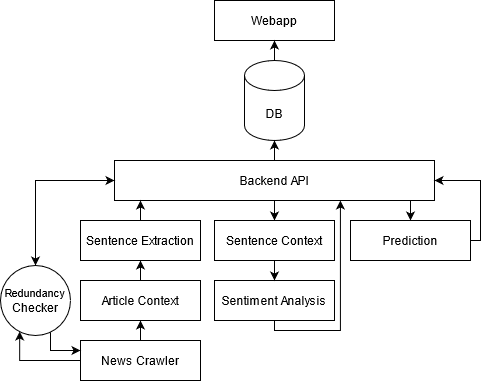
\includegraphics[width=0.7\textwidth]{images/upload/Architecture_origonal.png}
        \caption{Original Architecture}
        \label{fig:architecture_orginal}
    \end{figure}
    
    As work on the project continued it became clear that improvements could be made to original design, shown in Figure \ref{fig:architecture_orginal}. The components were too tightly coupled to one another, since each depended on one another to manage the flow of data and communication. Additionally, since all components attempted to access the database simultaneously it could potentially cause strain on the backend API and database. To remedy these concerns the system architecture was revised to better tackle these issues. 
    
    \begin{figure}[!h]
        \centering
        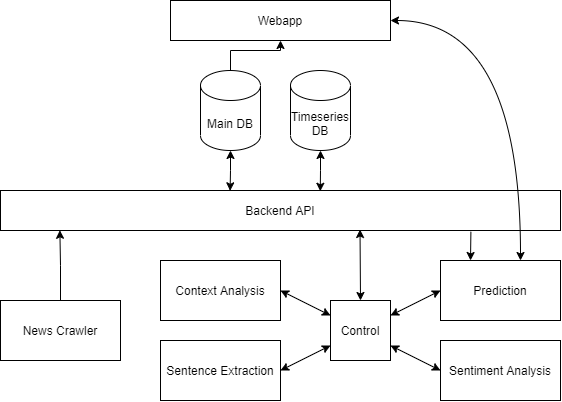
\includegraphics[width=0.6\textwidth ]{images/upload/architecture_reviz.png}
        \caption{Revised Architecture}
        \label{fig:architecture_reviz}
    \end{figure}
    
    The revised architecture, shown in Figure \ref{fig:architecture_reviz}, mitigates the strain on the database by reducing the amount of backend components that require access to the database. This is achieved through turning the sentiment analysis, sentence extraction, context analysis and stock prediction components into services that provide functionalities to a control component which manages the flow of data between the backend components and the database. As mentioned, Figure \ref{fig:architecture_reviz} shows the revised architecture and its various components. Each box represents a separate component with the lines showing which ones they interact with and how data flows between them. The revised architecture consists of the following components:
   
    \begin{itemize}
        \item \textbf{Backend API}: Backend interface to the main database and time-series database.
        \item \textbf{Context Analysis}: Determines what companies are being talked about in a given article or sentence.
        \item \textbf{Control}: Controls interaction and data flow between the backend API and backend components. 
        \item \textbf{Main DB}: Stores data on companies, sources, articles and sentences.
        \item \textbf{News Crawler}: Crawlers articles from given sources.
        \item \textbf{Prediction}: Predicts future stock price for a given company.
        \item \textbf{Sentence Extraction}: Extracts sentences from articles.
        \item \textbf{Sentiment Analysis}: Analyses sentences and awards sentiment score.
        \item \textbf{Time-series DB}: Stores time ordered data points on companies used in prediction component .
        \item \textbf{Webapp}: Frontend user interface in the form of a webapp.
    \end{itemize}
    
    
    \section{Backend Components}
    \label{Design:Back_comp}
    The backend components centre around a central management component, with the various other components acting as microservices that fulfil one key role or purpose. This allows for a separation of concerns as different components are contained within themselves and have limited or no interaction with one another. Each of the backend components has been designed to have the characteristics of a microservice as shown in \cite{microservices}; more specifically each component was designed with the following characteristics in mind: 
    
    \begin{itemize}
        \item \textbf{"Small and Focused"}: each component tackles only a few problems and remains small in size and scope, this prevents components becoming overlay complex and allows for a more manageable code base.
        
        \item \textbf{"Loosely Coupled"}: Each component can operate independently of each other, without the need for other components to be running. 
        
        \item \textbf{"Bounded Context"}: Each component has a specific purpose or domain and does not overlap or interfere with another component's domain.
    \end{itemize}
    
        \subsection{News Crawler}
        % REDONE
        Requirement \textbf{\#1} calls for the ability to collect news articles for the system to process and ultimately make predictions from them. To fulfil this functionality it was decided that a news crawler would be developed to crawl and collect news articles from a list of predefined sources. Unlike the other backend components, which act as rest microservices to the control component, the News crawler instead communicates directly to the backend API as shown in architecture diagram \ref{fig:architecture_reviz} and constantly inputs new articles into the system. The crawler will take articles from established news sites RSS feeds, specifically financial, market news and technology RSS feeds as these feeds are the most likely to provide articles that will be useful to the system. The crawler will loop through these predefined sources until a new article is found, and will then sleep for five minutes before doing the same again. This is to prevent the crawler from over calling the RSS feeds but also allowing it to keep up with the twenty-four-hour news cycle. Seven news sources were selected to be crawled from:
        
        \begin{multicols}{2}
        \begin{itemize}
            \item Wall Street Journal \citep{source:WSJ}.
            \item TIME \citep{source:TIME}.
            \item BBC \citep{source:BBC}.
            \item CNBC \citep{source:CNBC}.
            \item Financial Times \citep{source:FinancialTimes}.
            \item Fortune \citep{source:Fortune}.
            \item Economic Times \citep{source:EconomicTimes}.
        \end{itemize}
        \end{multicols}
        
        These sources were selected due to them all being established and well-known sources of news and information that many people use daily. Each source has various RSS feeds that provide different categories of information. Financial, Technology and Market streams were selected from the site to better gather articles that will be most useful to the system.
        
        \subsection{Sentence Extraction}
        \label{des:sentence}
        % REDONE
        Requirement \textbf{\#4} describes the functionality of being able to extract meaningful sentences from articles. This is achieved through the sentence extraction component that, when given an article's transcript, returns a list of sentences that exist in the article. Extracting sentences from articles rather than simply performing analysis on the articles as a whole was decided upon as it allows for a more manageable task that can capture the different contexts and sentiments throughout each sentence. Extracting sentences from a text can be achieved through various methods. 
        
        \begin{itemize}
            \item The first sentence extraction method considered was a Regex parser which through regular expressions analyzing punctuation in a sentence would identify the beginning and end of a sentence.
            \item The second method considered was to use a pre-trained neural language model to split the article into sentences provided by existing technologies.
        \end{itemize}
        
        The pre-trained model was decided upon as, although we would have less control over the inbuilt model, we would save time on implementation. As mentioned at the start of section \ref{Design:Back_comp} the backend components were designed to act as microservices. The sentence extraction component focuses on the single task of sentence extraction keeping it "small and focused" \cite{microservices} while also not interfering with any other component's domain and does not require other components to operate. The component exposes one function that when sent an article divides the transcript of the article into sentences using the sentence extraction model then returns the list of sentences:

        \begin{itemize}
            \item \textbf{Input}: Transcript of Articles.
            \item \textbf{Output}: List of sentences.
        \end{itemize}
                
        
        \subsection{Context Analysis}
        \label{des:context}
        %REDONE
        Requirements \textbf{\#3} and \textbf{\#7} call for context identification that allows companies to be identified in articles and sentences. This is done through the context analysis component which uses Named Entity Identification to find entities being discussed in articles and then discover if any of those entities are companies. As discussed in \ref{background:NER} there are different approaches to named entity recognition (NER) and various technologies that exist to support it. It was decided that multiple pre-existing NER technologies would be evaluated and implemented into the context analysis component. Further details on this evaluation can be found in chapter \ref{eval:context}. The context analysis component exposes two separate functions that both provide named entity recognition. The first of these is for articles when they first enter into the system. The context analysis component creates a list of possible entities mentioned throughout the article. 
        
        \begin{itemize}
            \item \textbf{Input1}: Transcript of article.
            \item \textbf{Output1}: List of potential companies.
        \end{itemize}
        
        The second function the context analysis component provides is entity recognition for sentences. If one or more companies are found using the named entity recognition model then they become the potential context for the sentence or, if not, then the sentence uses its parent article context list. The component attempts to match the potential entities to companies within the database and returns the stock code if successful. 
        
        \begin{itemize}
            \item \textbf{Input2}: Sentence Text.
            \item \textbf{Output2}: Stock code of companies.
        \end{itemize}
        
        Returning to the characteristics described in section \ref{Design:Back_comp} we can see the component focuses on the task of context analysis and does not require other backend components to operate. Additionally, it provides only two key functionalities keeping it small and focused.
        
       
        \subsection{Sentiment Analysis}
        % REDONE
        Requirement \textbf{\#5} and \textbf{\#8} Relate to the sentiment analysis which calls for the ability to award a sentiment score to a piece of text. This is achieved through the sentiment analysis component which processes sentences and awards a polarity score. Discussed in chapter \ref{background:Sentiment} there are various approaches and techniques to sentiment analysis that could be applied to this project. Similar to the context analysis component in section \ref{des:context}, we used existing technologies to provide the sentiment analysis model. Once a working version of the component was built, we then returned to this model and evaluated it by comparing it to other technologies and systems. More on this evaluation can be found in chapter \ref{eval:sentiment}. The sentiment component exposes one function that, when given a piece of text, returns a polarity score ranging from one to negative one, with one being extremely positive and negative one being extremely negative. The scores given here are important as they found the basis of the stock predictions made in the prediction component \ref{prediction}
        
        \begin{itemize}
            \item \textbf{Input}: Sentence text.
            \item \textbf{Output}: Polarity score between 1 and -1.
        \end{itemize}
        
        Again, relating this back to the features described at the start of section \ref{Design:Back_comp}, the sentiment analysis component is small and bounded to a single context as it only fulfils one function of analyzing sentiment in text and does not require other components to operate. 
        
        \subsection{Stock Prediction}
        \label{prediction}
        The prediction component is the culmination of the previous components and satisfies requirements \textbf{\#6} and \textbf{\#9} need for the ability to predict the price of a stock for a given day. The prediction component initially contained two API calls. The first is used to turn sentences into data points to be stored in a time-series database, see \ref{TimeseriesDB}, and also to be used in stock prediction. The second API call is the main prediction method that, when given a company's stock code, will retrieve all existing data points on that company from the time-series database and then go through the following steps:
        
        \begin{enumerate}
            \item Retrieve the historical financial data from the given company starting from the date the first article was crawled on the company to the current date.
            \item Average together data points that were crawled at the same time.
            \item Using the known sentiment on days an article was crawled, build a model to impute missing sentiment for days no article was crawled for the company.
            \item Using the sentiment and stock price for each day to predict the stock price of the company for the next thirty days.
        \end{enumerate}
        
        Once this list of future predictions is created, the prediction component also checks to see if the average future stock price is higher or lower than the current stock price. This difference in price forms the basis of the \textit{Verdict} that each company is given. Three different verdicts can be awarded to a company with them being:
        
        \begin{itemize}
            \item \textbf{Hot} The predicted value of the stock has seen a noticeable increase therefore suggesting a user should purchase stock in the company.
            \item \textbf{Not} The predicted value of the stock has seen a noticeable decrease therefore suggesting a user should not purchase stock in the company.
            \item \textbf{Hold} There is no noteworthy difference in the price of the stock and therefore a user should hold onto the company's stock if they have any.
        \end{itemize}
        
        Additionally, the prediction component was also extended to fulfil requirement \textbf{\#11} by exposing another API call that allows for custom predictions to be made. Custom predictions follow the same steps as the standard prediction method however the starting date and days into the future are given by the user.
        
        \begin{itemize}
            \item \textbf{Input}: Stock code of company.
            \item \textbf{Output}: Prediction results and verdict.
            \smallskip
            \item \textbf{Input}: Stock code of company, time frame.
            \item \textbf{Outpu2}: Prediction results.
        \end{itemize}
        
        
        \subsection{Control Component}
        \label{Control Component}
        The Control component is critical to the overall systems function as it is responsible for communicating with the various components, in order to process articles and sentences in the correct order and send them to the correct components. Unlike the previous components, the control component is not structured as a microservice and instead, it houses the business logic that manages communication between the varying components and the backend API. To prevent the component from causing strain on the database, the control component waits for a notification from the main database whenever a new Article or sentence enters the system. When it receives a notification, the component queries all sentences and articles that do not have the \textit{Done} status, see \ref{Main Database} for more information, and begins to process them accordingly.
        
        
        \subsection{Backend API}
        \label{Backend API}
        The backend API acts as the gateway between the Backend components and the database providing various API calls with different functionalities. The Backend API was first designed to support interaction with the Article, Company, Sentence, Source and Tag tables, with it opening up API's that allowed query, editing and inputting of data into these tables. These API calls were first detailed on Swagger Hub \citep{website:Swagger} so that they could be reviewed and changed before work began on implementing it. This ensured that all the required API calls were accounted for and organised. Later in the project, the API was extended to support API calls that communicate to the Time-series database, discussed in section \ref{TimeseriesDB}. These API calls were designed to only ask for a start date along with a company stock code with all the logic being managed by the Backend API itself. The full documentation of the backend API can be found here:
        \begin{itemize}
            \item \url{https://app.swaggerhub.com/apis-docs/HotOrNot/HotOrNot/1}
        \end{itemize}
        
        
    \section{Database}
    \label{Datbase}    
    Requirement \textbf{\#2} relates to the system's database that stores a multitude of information including articles collected from new sources, sentences extracted from those articles and information on given companies. Additionally, the prediction component also needed an easier way to retrieve sentences in a given time frame for a given company. It was therefore identified that two separate databases would need to be created. One to store the more general information on companies, articles and sentences and another that would store data points, created from sentences, in a time-series format. 
    
        \subsection{Main Database}
        \label{Main Database}
        The main database is used to store the general information on companies, news sources, tags and any articles found by the news crawler along with their resulting sentences. The following ER diagram shown in Figure \ref{fig:db_schema_main} was created as an overview for how the main database and its respective tables work:
        
        \begin{figure}[!h]
            \centering
            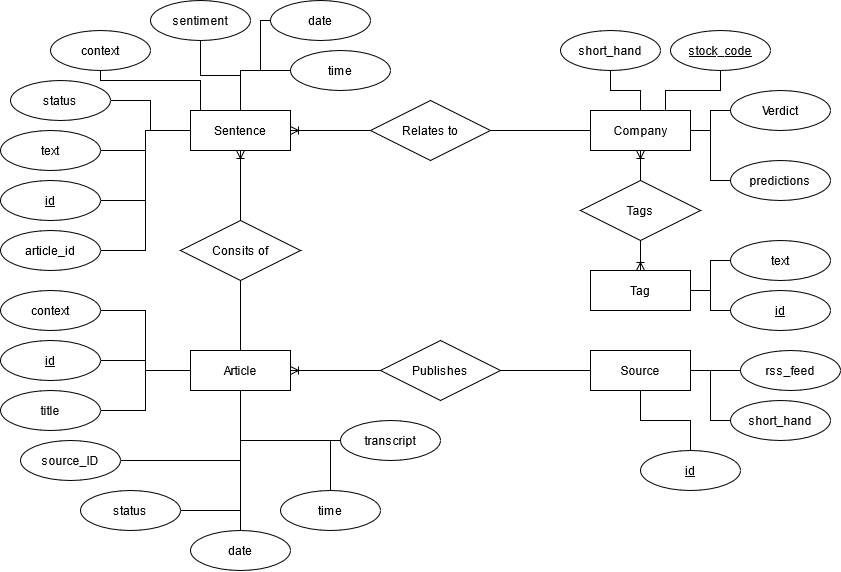
\includegraphics[width=0.7\textwidth]{images/upload/ER full.png}
            \caption{Main Database ER diagram.}
            \label{fig:db_schema_main}
        \end{figure}
        
        Sources are the news sites that articles are gathered from, with every article that is crawled linking to one of these news sources. Each article stores various information such as the time it was crawled, title, article transcript, etc. When sentences are extracted from an article, they are stored in the Sentence table, with each sentence storing its parent article ID, along with its text, sentiment and context. The company table stores the stock code and shorthand of all the companies in the system with various tags and sentences linking to a given company. Additionally, the article and sentence tables were extended to have a 'status' field that links to the current stage of the process of either the article or sentence. The status that an article could take are:
        
        \begin{itemize}
            \item \textbf{Context}, The article is waiting to be processed by the context identification component
            \item \textbf{Sentences}, The article is waiting to have its sentences extracted
            \item \textbf{Done}, The article has been completely analyzed
        \end{itemize}
        
        The various statuses for the sentences are as followed:
        
        \begin{itemize}
            \item \textbf{Context}, The sentence is waiting to be processed by the context identification component
            \item \textbf{Sentiment}, The sentence is waiting to be processed by the sentiment analysis component
            \item \textbf{Pred}, The sentence is waiting to be translated into a data point by the prediction component
            \item \textbf{Done}, the sentence has been completely analyzed
        \end{itemize}
        
        The status field was added for two main reasons. Firstly, it allows for easier lookup of which articles and sentences have been completely analyzed and which have not. Secondly, it supports the control component, \ref{Control Component}, in determining the current of analysis of the given article or sentence. Additionally, both articles and sentences can receive the \textbf{Blocked} status, meaning that during context analysis, no company was registered and as such no more analysis is required. This prevents useless articles and sentences from being processed.  
        
        \subsection{Time-series Database}
        \label{TimeseriesDB}
        % REDONE, sort of
        The prediction component needs to have fast access to the sentiment data for a given company. Although simply querying a sentence's sentiment by a company. and ordering by time would produce the same result, a time-series database would reduce query times significantly. Therefore, it was decided that a separate time-series database containing data points for the perdition component. Data points contain the time the sentence it refers to was crawled, the sentence's ID, sentiment, stock code and company closing price at the time it was crawled. Having a time-series database allows easy lookup and referral to a company's sentiment history with the data already ordered for the components of the prediction.  
       
       
    \section{Frontend}
    The frontend component is the web app that allows the users to view and interact with the data collected on companies. Using inspiration from the competitor sites reviewed in section \ref{Competitors} it was decided that there would be two main pages. A home page, as mentioned in requirement \textbf{\#13}, that presents a shortlist of all the companies on the site along with their \emph{Hot or Not} rating along with a central search bar that allows user to filter and search through the companies. The second page is the company specific that displays relevant information on the company such as stock price, business summary, financial data, etc as well as a graph of previous stock price along with a prediction on the future of the stock price. 
        
        \subsection{Prototypes}
        Before implementation of the frontend, a series of wireframes were developed in an iterative process for the two pages on the webapp. This ensured that all requirements were represented and accounted for in the design of the webpage. 
        
        \subsubsection{Homepage}
        \label{Homepage}
        The Homepage is the first place a user will land when going to the website and therefore required careful planning on the design and layout of the page. Additionally, the page must be able to fulfil requirement \textbf{\#15} by having a search bar to find companies and requirements \textbf{\#19} and \textbf{\#16}, by having tags and filter options for searching.
        
        \begin{figure}[!h]
            \begin{subfigure}[b]{0.4\textwidth}
                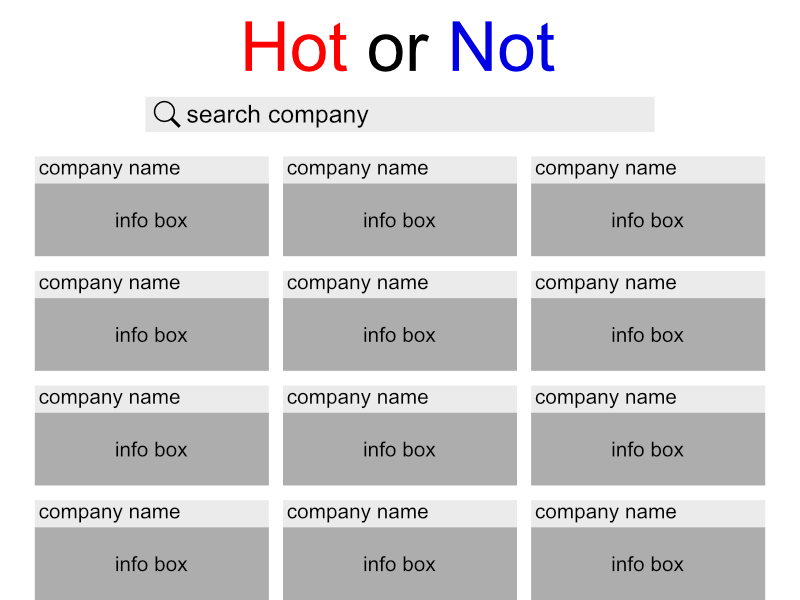
\includegraphics[width=\textwidth]{images/upload/Home Wireframe.png}
                \caption{Initial wireframe.}
                \label{fig:homepage_initial}
            \end{subfigure}
            \hfill
            \begin{subfigure}[b]{0.4\textwidth}
                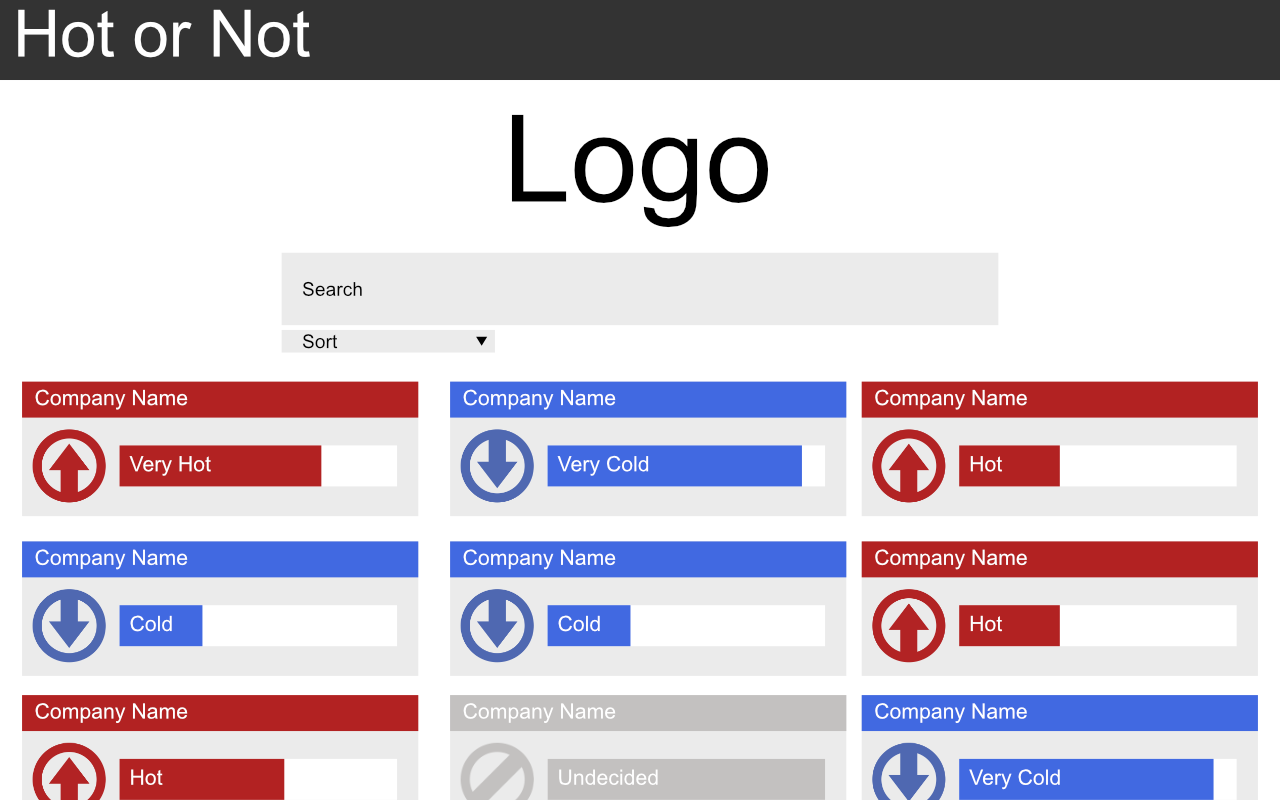
\includegraphics[width=\textwidth]{images/upload/Home-wireframe2.png}
                \caption{Revised wireframe.}
                \label{fig:hompage_revised}
                \end{subfigure}
            \caption{Homepage wireframes}
        \end{figure}
        
        A minimalist design was desired that showed the user enough information to make meaningful assumptions on a company just from a glance at the homepage but wouldn't show too much information and over-complicate or overcrowd the homepage. The initial design of the company page shown in figure \ref{fig:homepage_initial} began the idea of having small information boxes for each company along with the ability to search through these information boxes through a search bar at the top of the screen. This design was then expanded, shown in figure \ref{fig:hompage_revised} by having a Hot to Not meter for each company, giving an indication of how well each company is predicted to perform without complicating the design. Moreover, the search bar was made a larger and more prevalent part of the homepage, along with a colour scheme and icons for each potential verdict a company could receive; Hot, Not or Hold. 
        
        \subsubsection{Company Page}
        The company page allows the user to see information on a given company and contains many critical requirements that must be completed for the system and project to succeed. The wire frames for the company page started with layout, see Figure \ref{fig:Company_itsss} and how the core sections of the company page should fit together. For requirement \textbf{\#22} the company page had to show the different sentences found on the given company and deciding where this should be placed was one of the difficulties when designing the company page. Iteration \ref{fig:company_it3} was finally elected to build upon further as it was felt it provided a simplistic layout and didn't emphasise the article snippets while also giving them the screen space they needed
          
        \begin{figure}[!h]
            \begin{subfigure}[b]{0.3\textwidth}
                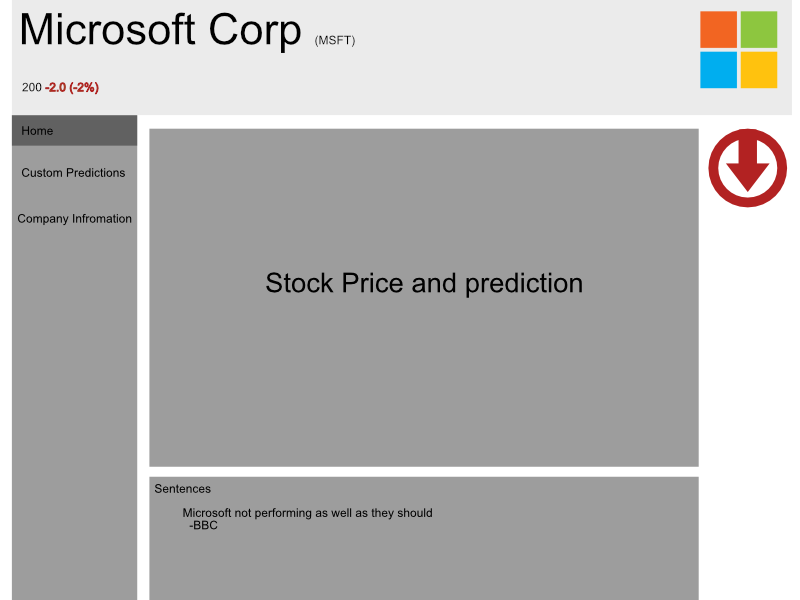
\includegraphics[width=\textwidth]{images/upload/Company-Wireframe1.png}
                \caption{Iteration One.}
                \label{fig:company_it1}
            \end{subfigure}
            \hfill
            \begin{subfigure}[b]{0.3\textwidth}
                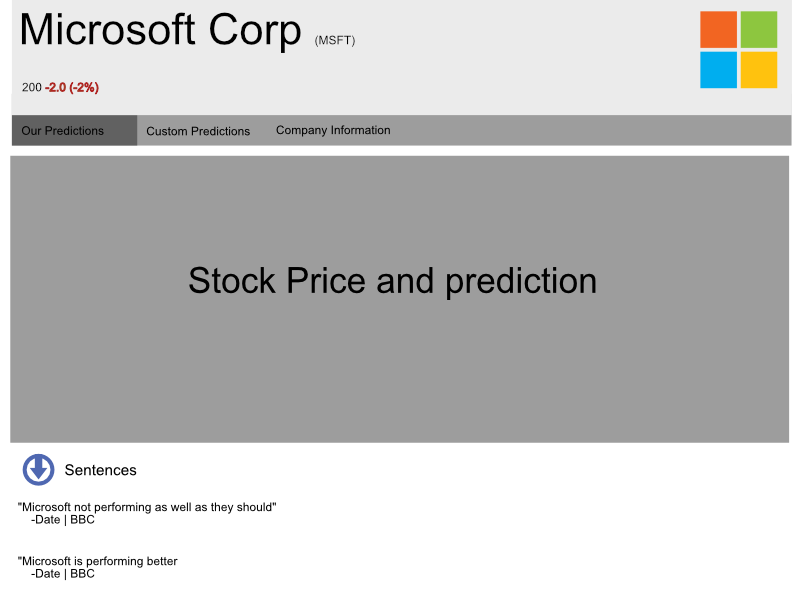
\includegraphics[width=\textwidth]{images/upload/Company Wireframe 3.png}
                \caption{Iteration Two.}
                \label{fig:company_it2}
            \end{subfigure}
            \hfill
            \begin{subfigure}[b]{0.3\textwidth}
                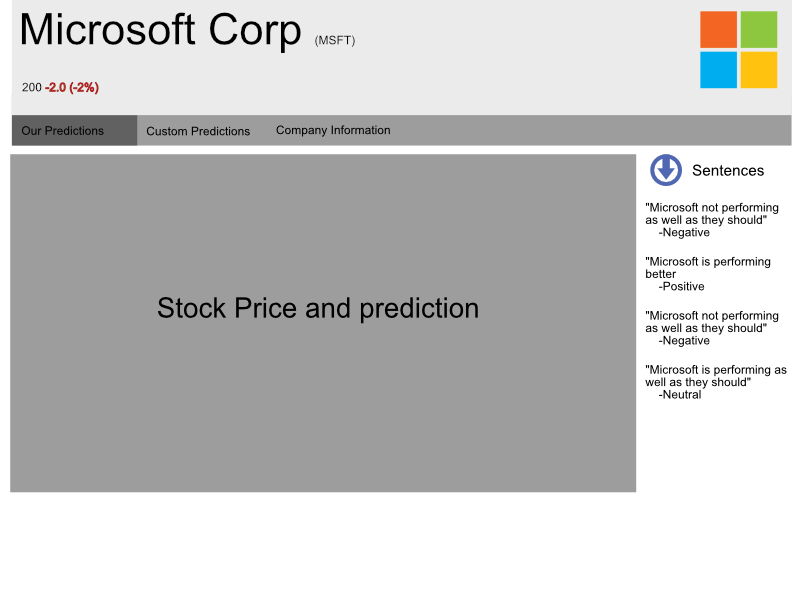
\includegraphics[width=\textwidth]{images/upload/Company Wireframe 2.png}
                \caption{Iteration Three.}
                \label{fig:company_it3}
            \end{subfigure}
            \caption{Company page wireframe iterations}
            \label{fig:Company_itsss}
        \end{figure}
        
        The next task was to design how each tab on the company page should be laid out. The prediction tab shown in Figure \ref{fig:company_tab1} is where systems default prediction for the stock price is shown and gives a graph of the previous prices thus ensuing requirements \textbf{\#18} and \textbf{\#17} are represented. The information tab shown in Figure \ref{fig:company_tab2} was added, in order to fulfil requirement \textbf{\#21} and is home to general information about the company, such as the company's logo, sector and financial information. The final tab shown in Figure \ref{fig:company_tab3} is where users can create custom predictions for the company's stock price by telling the system what start and end date should be used.
        
        \begin{figure}[!h]
            \begin{subfigure}[b]{0.3\textwidth}
                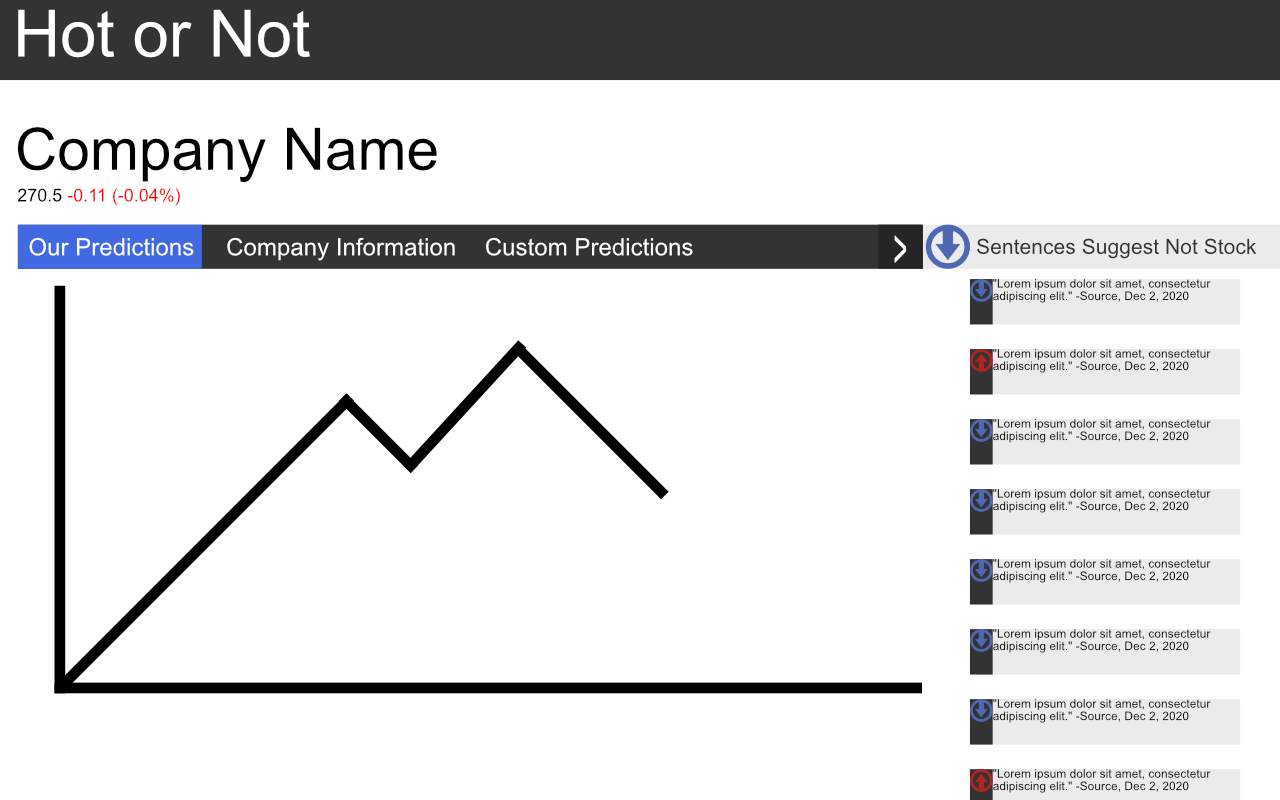
\includegraphics[width=\textwidth]{images/upload/Company-wireframe 4.png}
                \caption{Prediction Tab.}
                \label{fig:company_tab1}
            \end{subfigure}
            \hfill
            \begin{subfigure}[b]{0.3\textwidth}
                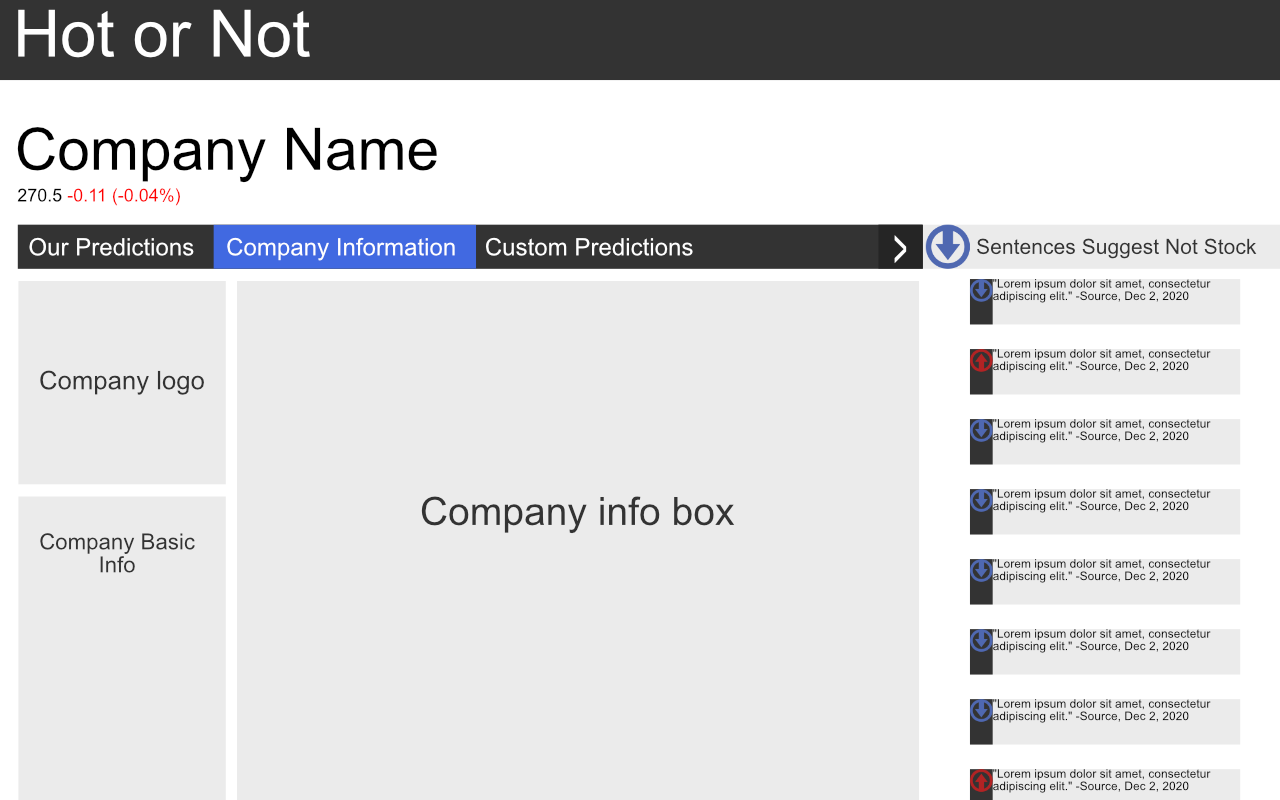
\includegraphics[width=\textwidth]{images/upload/Comapny-wireframe 6.png}
                \caption{Information tab}
                \label{fig:company_tab2}
            \end{subfigure}
            \hfill
            \begin{subfigure}[b]{0.3\textwidth}
                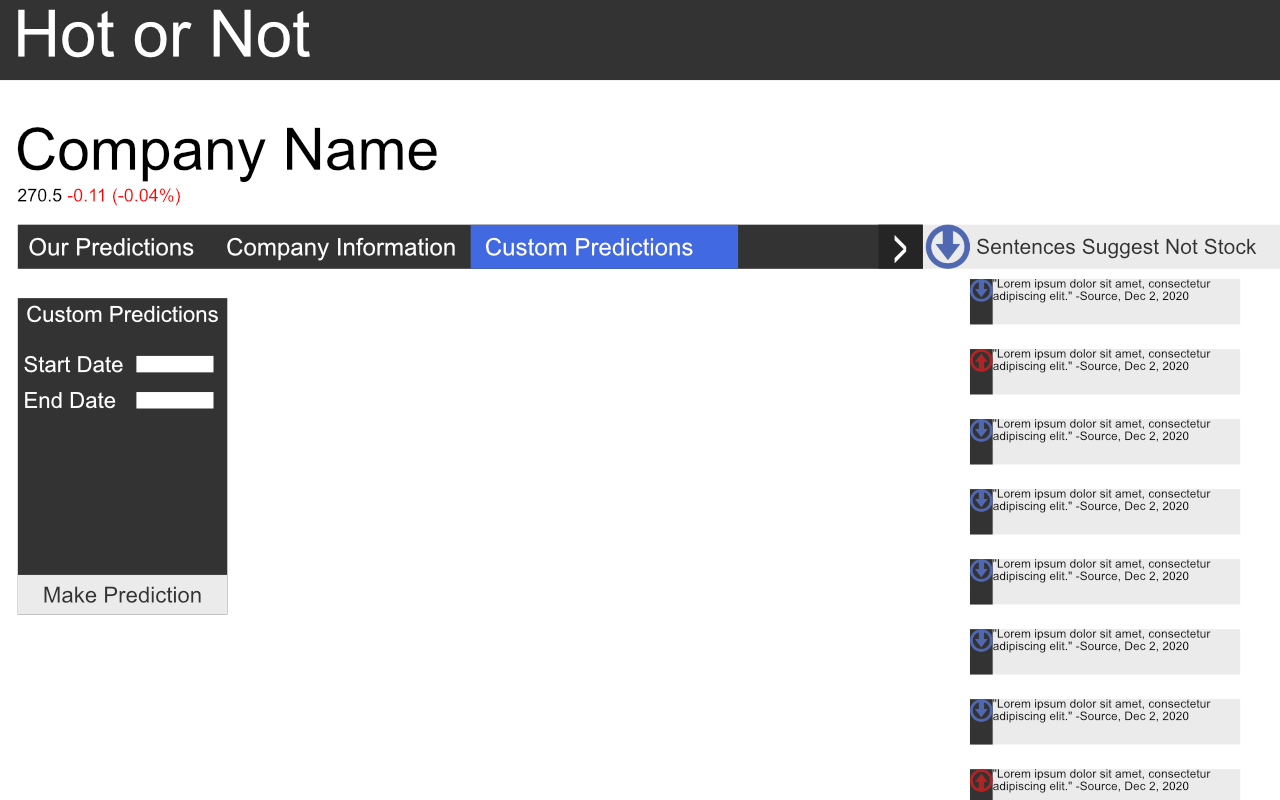
\includegraphics[width=\textwidth]{images/upload/Company-wireframe 5.png}
                \caption{Custom Prediction tab}
                \label{fig:company_tab3}
            \end{subfigure}
            \caption{Company page separate tab wireframes}
        \end{figure}
        
    \section{Summary}
    This chapter highlights and justifies the design decisions made in regards to the project. An overview of the system's architecture along with a description of the operation and purpose of each component is provided. The design choices and overview of the database system along with the process for designing the frontend through an iterative wireframe approach was also detailed. 
\chapter{Implementation}
\label{Implementation}

% % For off the shelf technologies, add in how they work

% Add in key challenges, tell story

    \section{Software Engineering Process}
    
        \subsection{Github}
        Github \citep{website:Github} was used to store and manage version control of the project. Moreover, Github's issue system was used to manage to do tasks throughout the project. The project's repository can be found here:
        \begin{itemize}
            \item \url{https://github.com/2312420/lvl4-project} 
        \end{itemize}
          
            \subsubsection{Issue Strategy}
            Issues were created based on a single overarching goal that had to be completed. Within the Issue, various tasks and steps were added that needed to be completed to achieve this goal. Issues would be created at the start of each week with the goal being to complete issues by the end of the week. This helped to keep a manageable number of issues at any given time and also allowed for easy oversight of how many issues remained from previous weeks. 
            
            \subsubsection{Commit and Branching Strategy}
            Commits were to be made every time one of the tasks in an issue was completed or an important step towards completing a task was taken. Commit messages were also kept small and concise in order to reduce confusion. A master and develop branch were initially created when work began on the project and these two branches existed throughout the projects life-cycle. When work began on an Issue, a new feature branch was created from develop. When the feature and goals for that issue had been achieved, the branch was merged into develop.
            
            All branches were named to abide by the following naming convention: "<name of issue / area being worked on>-<issue id>". For example Issue, \#58 "Prediction Restructure" branch would be named "Prediction\_Restructure-58". Merge requests were only ever made through the GitHub website so if any merge conflicts were raised, they could be easily solved. Each merge request was also referenced to the issue or issues it solved. Having a core branch and commit strategy helped to prevent the project repository from becoming too complex with an overabundance of branches while also still keeping the main and develop branches safely.
            
            \subsubsection{Repository Insights}
            Throughout the project's life cycle, 37 issues were created, 42 branches and branch merges were issued and 274 commits were made. Figure\ref{fig:Git_commmits} shows the commits made throughout the project. As we can see commits and work on the project were made consistently across the year:
            
            \begin{figure}
                \centering
                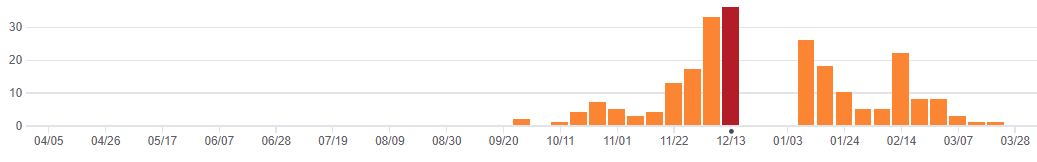
\includegraphics[width=\linewidth]{images/Commits.png}
                \caption{Overview of commits made to the project repository}
                \label{fig:Git_commmits}
            \end{figure}
            
        \subsection{Confluence}
        To organise weekly meetings and project notes, confluence \citep{website:confluence} was used, as it provides a whole host of note-taking features and allows for notes to be referenced and linked to one another to create a wiki for the project. A central page was set up for the project that contained connections to the various weekly notes. A project road map \ref{fig:Confluence_Roadmap} was also set up that contained a rough outline of what was done in each week and what was projected to be done in the weeks to come. 
        
        \begin{figure}[!h]
            \centering
            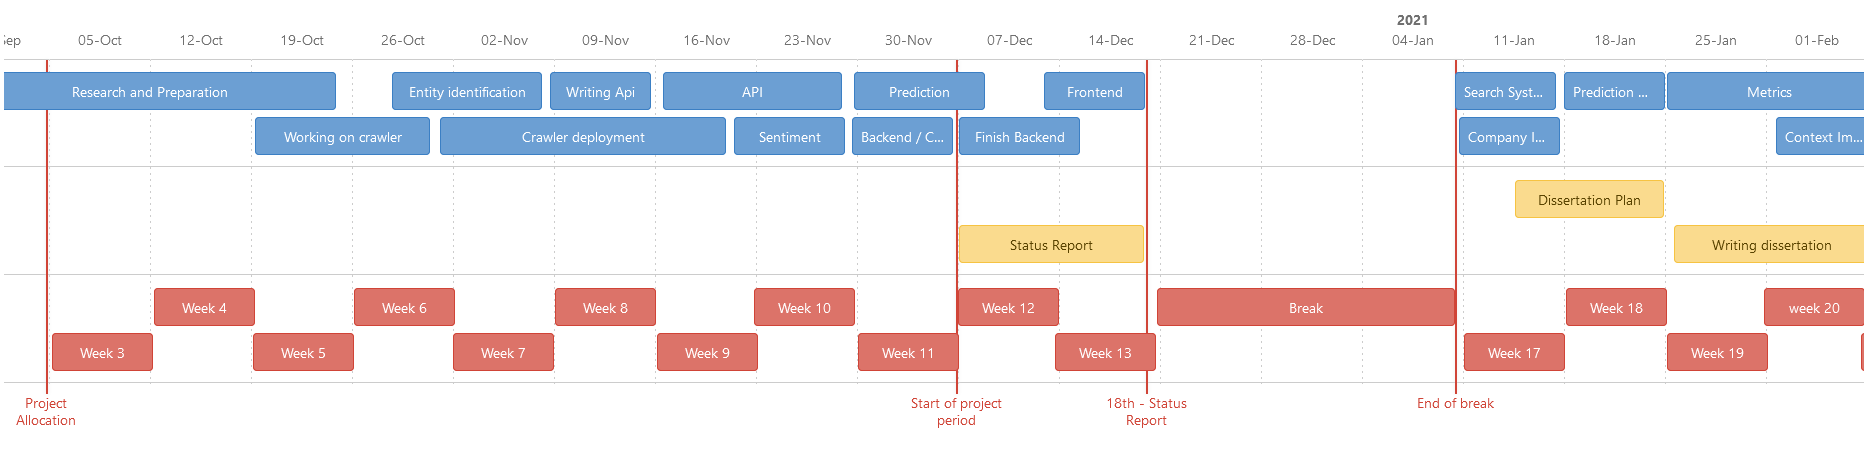
\includegraphics[width=0.9\linewidth]{images/upload/Roadmap.png}    
            \caption{Confluence Roadmap}
            \label{fig:Confluence_Roadmap}
        \end{figure}
        
        Additionally, on this home page was a list of all the project's requirements along with their importance (Must, Should, Could") and status (Done or Todo). This served as a constant reminder of the various key aspects of the project that still needed done and helped to stop the project from getting off-track or too focused on one requirement. 
        
        
    \section{Backend Implementation}
    Before the web app and its features could be created, the backend system first had to be up and running and therefore that is where the focus lay for the first months of the project. The backend components were built using Flask \citep{technology:Flask}, which allows the components to open up defined API calls.
    
        \subsection{News Crawler}
        % REDONE, sort of
        The news crawler is responsible for collecting articles from various sources, which will be processed and used throughout the system. Having data to test and work with while developing the other components was critical. It was therefore decided that the news crawler should be created first, since it is the logical starting point for articles in the system and provides access to this data. The crawler was implemented using the python library Newspaper3k \citep{technology:Newspaper} which provides simple methods and functions to scrape articles from News-sites RSS feeds. The news crawler will request articles from the various News sites until no new articles are found, when this happens the crawler sleeps for five minutes so as to not overload requests to the various sources. The Newscrawler communicates directly with the database through the backend API, inputting any new articles it manages to crawl
        
        \subsubsection{Redundancy} To prevent the same Articles from being inserted into the system, Articles are first put into a hash function that takes the first word of the article, the title of the article and the last word of the article to produce a unique ID. The article can then only be inserted into the system if this ID does not already exist.
        
        \begin{itemize}
            \item \textbf{Output}: \{title: "Stocks Today", transcript: "Apple's stocks fall today. Microsoft's stocks rise today", source\_id: "4"\}
        \end{itemize}    
            
        \subsection{Sentence Extraction}
        %REDONE
        The sentence extraction component is used to take the transcript of an article, extract the sentences from that article and return the list of sentences. The first step in creating the component was to implement the sentence extraction model which carries out the main function of separating the article into individual sentences. As mentioned in section \ref{des:sentence}, the extraction model was to be implemented using a pre-built model. Multiple technologies were considered, however NLTK \cite{Technology:NLTK} was decided upon as it offered extensive documentation, along with fast and simple implementation. NLTK provides multiple pre-trained models, each trained using a different data set. NLTK's Punkt sentence tokenizer was used to divide text into a list of sentences. This works by using an unsupervised learning algorithm which is trained in using large volumes of text. This algorithm develops a model which uses keywords, punctuation and phrases to divide text into sentences. With the sentence extraction method complete, the next step was to create the flask framework which exposes the necessary API calls for the system. The sentence extraction component contains one API exposed on its port, so that when given an article object in the form of a JSON, it returns a JSON of the sentences in the article.
        
        \begin{itemize}
            \item \textbf{Input}: \{transcript: "Apple's stocks fall today. Microsoft's stocks rise today"\}
            \item \textbf{Output}: \{["Apples stocks fall today", "Microsoft's stocks rise today"]\}
        \end{itemize}
        
        
        \subsection{Context Analysis}
        %REDONE
        The context analysis component is used to understand what company is being discussed in each article or sentence. The context analysis component when given an article needs to return a list of potential companies and when given a sentence needs to return the stock code of the company being discussed. As mentioned in section \ref{des:context} the context analysis component uses named entity recognition to identify the companies being discussed. This model was implemented using Spacy \cite{technology:Spacy} through its inbuilt word tokenization and NER model. Spacy was used initially as it had extensive documentation and could be implemented easily, however other technologies would be considered when the time came to evaluate the component. Spacy's named entity recognition model is trained using blogs and news articles and, as detailed in its documentation \cite{spacy_ner}, uses a neural network based approach to give analysis of sentences and label potential entities. With the named entity recognition model implemented, the context analysis component then separates out entities which do not have the "ORGANISATION" tag, as we are only interested in articles discussing companies. With the component able to identify companies being discussed in a text, the next step was to implement the flask framework and expose the two API calls for article and sentence context analysis. Articles and sentences are handled separately by the component:
        
            \subsubsection{Article Context}
            The article API call will use the NER model to analyze the transcript of the article and find any organisation entities it contains. When sent a JSON of the article, it will return the JSON with an additional "context" field which contains a list of potential entities being discussed in the article.
            
            \begin{itemize}
                \item \textbf{Input}: \{transcript: "Apple's stocks fall today. Microsoft's stocks rise today."\} 
                \item \textbf{Output}: \{transcript: "Apple's stocks fall today. Microsoft's stocks rise today." context: [Apple, Microsoft]\} 
            \end{itemize}
            
         
            \subsubsection{Sentence Context}
            The sentence API call also uses the NER model to analyze the text of the sentence to find any organisation entities it contains. If one or more organisations are found then that will be used as the potential context of the sentence. If no organisation is found then the sentences parent article context list is used instead. This is done to capture sentences that do not necessarily mention a company, but relate to the overall article context. Once the potential context of the sentence has been decided, it then needs to be linked to an item in the database. This was achieved by fuzzy querying the company database to find company short-hands that are similar to the potential entities. If the query manages to produce a valid result, then the stock code of that company becomes the context for the sentence. The text and new context of the sentence is then returned.
            
            \begin{itemize}
                \item \textbf{Input}: \{text:"Microsoft's stocks rise today"\}
                \item \textbf{Output}: \{text:"Microsoft's stocks rise today", context: "MSFT"\}
            \end{itemize}
            
            \subsubsection{Improvements}
            The context analysis component was improved by evaluating the effectiveness of the named entity recognition model, comparing the Spacy model to other technologies. The Stanford NER Libary, stanza \citep{technology:Stanza}, at the time of development contained more advanced fully neural network model that provided the best results, so the component was updated to use that model instead. More detail for the evaluation of the component can be found in chapter \ref{eval:context}
            
            
        \subsection{Sentiment Analysis}
        %REDONE
        The sentiment analysis component is used to analyze the text of a sentence and award a polarity score ranging from -1 to 1 on the sentiment of that text. It is one of the more important components as the score awarded here will be used in the stock prediction component. The sentiment analysis model was initially built using the python library VADER sentiment \citep{Technology:Vader}. This library provides open-source sentiment analysis tools to measure the sentiment intensity of a given text. This is done through a lexicon that scores positive and negative sentiment intensities for thousands of different words. This lexicon is then used to measure the amount of positive and negative words in a sentence and award a sentiment score. Once the VADER sentiment model was implemented, the next step was to again implement the framework and expose the API call that, when given text, returns the sentiment score. 
        
            \begin{itemize}
                \item \textbf{Input}: \{text:"Microsoft's stocks rise today"\}
                \item \textbf{Output}: \{score: "0.8"\}
            \end{itemize}
        
            \subsubsection{Improvements}
            Though VADER sentiment proved useful to build the initial sentiment analysis component we needed to ensure that the sentiment scores had a high degree of accuracy. Therefore VADER sentiment was compared to technologies in the paper Choosing your weapons: On sentiment analysis tools for software engineering research" \citep{7332508} mentioned in chapter \ref{Background}. The accuracy, precision and recall of each technology were measured, with Textblob \cite{technology:Textblob} providing the best results, the sentiment analysis component was then switch to use is sentiment model instead. Further details on the evaluation of the component can be found in chapter \ref{eval:sentiment}
        
       
       
        \subsection{Stock Prediction}
        The stock prediction component was one of the more complex and difficult parts of the system to implement and required significantly more time and work than the previous components. Sklearn \citep{technology:Scikit-learn} was used extensively throughout the component to provide the various predictions models needed.
            
            \subsubsection{Financial Data} The first step in creating the prediction model was to make it able to retrieve historical financial information about a given company. The python library Yfianance \citep{technology:yfinance} was used to retrieve financial information from Yahoo \citep{website:Yahoo}. Once the financial information is retrieved the component then gets the sentiment data collected on the company and combines the financial information and sentiment data into one. This proved difficult, as past a certain point financial data retrieved from Yahoo can only be collected by day rather than specific times. This required the sentient data to be averaged for each day before the combining process could begin. Once both data sets are ready a new data frame index by time is created, with the available financial and sentiment data filled in. 
            
            \subsubsection{Sentiment Prediction} The sentiment model is used to fill out the missing sentiment data in the previous data frame and to predict the future sentiment of the company. A sentiment model build using Sklearn's Bayesian Ridge regressor \cite{sklearn_bayes} uses known sentiment and financial data of the company to predict the missing sentiment data in the data frame. Once this is complete, the model then uses the dataframe to predict the future sentiment of the company by using the previous sentiment and the time separated into multiple features as training data. 
            
            \subsubsection{Stock Prediction} Once the dataframe with closing price, sentiment and time has been built, the component then moves onto predicting the potential future closing prices. Various models were evaluated to the best prediction results, with the final model being the Sklrean Random Forest Regressor \cite{sklearn_forest}, more information on this evaluation can be found in chapter \ref{eval:prediction}. A Random Forest Regressor is similar to a standard decision tree, in that it creates a tree of rules to decide the value of future data, however it has more randomness and variance to it, in order to avoid over fitting. 
            
            \subsubsection{Verdict}\label{Verdict} With the predictions having been made, the final step for the component is to analyze the data and award an overall verdict for the company. This is done by calculating the difference between the average of the predicted stock prices and the current stock price. If the difference is not greater than 0.5 or less than -0.5 then the stock is awarded the Hold verdict. A stock with a positive difference is awarded the Hot verdict whereas a stock with a negative difference is awarded the Not verdict. The difference, verdict and predictions are then returned. 
            
            \subsubsection{Custom Prediction and Restructure}
            The stock prediction component also had to facilitate user-made custom predictions. It was decided that a user would be able to define a start date and an end date and using any data in that time frame, the component would attempt to predict the stock prices. When the time came to implement this system, it became apparent that the stock prediction component had become confusing and disorganised with monolithic functions. It was therefore restructured with prediction models, data manipulation functions and common functions all being separated into their own files and directories. Additionally, various methods were expanded to accept a custom dates in order to better facilitate the custom prediction system. With this complete it a simple custom prediction function could be created with ease.

            \subsection{Overview} With the prediction system operational the stock prediction component was made to expose three API's using the Flask framework. The first API was the basic stock prediction used to determine the verdicts and information displayed on the web app:
            
            \begin{itemize}
                \item \textbf{Input}: \{stock\_code: "MSFT"\}
                \item \textbf{Output}: \{verdict: "HOT", predictions: [(01/04/2020, 102), ...]\}
            \end{itemize}
            
            The second is the custom prediction call that returns an ordered list of stock predictions between the start and end dates provided.
            
            \begin{itemize}
                \item \textbf{Input}: \{stock\_code: "MSFT", start\_date: "01\/04\/2020", end\_date:"01\/04\/2020"\}
                \item \textbf{Output} \{ predictions: [(01\/04\/2020, 102), ...] \}
            \end{itemize}
            
            Later in development the stock prediction component was expanded to contain an API call that transformed sentences into data points for the time series database. This was a straightforward implementation, with the input and output being:
            
            \begin{itemize}
                \item \textbf{Input} \{text:"Microsoft's stocks rise today", context: "MSFT", ..\}
                \item \textbf{Output} \{sentiment: "0.5", time: "01\/04\/2020", stock\_code: "MSFT, close\_price: 102"\}
            \end{itemize}
        
            
    \section{Database}
    The databases store the information that the system collects and process, with data split between the main database and the time-series database. The final schema for both databases can be found in Appendix \ref{fig:AP:schema}  
    
        \subsection{Main Database}
        The main database is used to store data on articles, sentences, companies and sources. PostgreSQL \citep{technology:PostgreSQL} was used to set up and manage the database as it is a well-known and long-established database management system with many features and good documentation to help guide the process of creating the database system. 
        
            \subsubsection{Tables}
            pgAdmin, a graphical extension that comes pre-packaged with PostgreSQL, was used to create the main database and the various tables it required. The Article, Sentence, Company and Source tables were created first with foreign key constraints linking them together. Each Article contained its source's ID, each sentence contained its parent article ID and each sentence also contained the stock code of the company it discussed, linking them together. When it came time to implement the Tag table, an intermediary table called Tags was created containing the ID of the tag and the stock code of the company it tagged. This created the desired many to many relationships between the Tag and Company table.
            
            \subsubsection{Inital Data}
            For the system to work, the company table had to be filled out with the shorthand names and stock codes of all the various companies. A data-set sourced from Kaggle, which contained the name and stock code of the S\&P 500 \citep{SP} was sourced to fill out this table. This data-set and more specifically, the S\&P 500 were selected due to them being some of the largest and most well-known companies in the world such as Apple, Amazon and Microsoft. The data set can be found here:
            \begin{itemize}
                \item \url{https://www.kaggle.com/dgawlik/nyse?select=securities.csv}
            \end{itemize}
            
        \subsection{Time-series Database}
        The Time-series database stores the data points used in the stock prediction component’s stock price prediction. Like the main database, the time-series database was implemented through PostgreSQL \citep{technology:PostgreSQL} however it only contains a single table which is the Datapoint table. To achieve the time-series functionality the Postgres extension Timescale \cite{technology:Timescale} was used is it allows for significantly faster and more accessible time-based queries to be made. 
        
            \subsubsection{Challenges}
            Timescale required a different version of PostgreSQL than the main database, meaning the databases had to be run on separate local servers. This meant more time went towards getting the time-series database operational before work could begin. Once complete, the Datapoint table had to be extended with Timescale's hypertables that partition the data of the Datapoint table to provide the fast time-based queries. This is done by having the Datapoint table indexed by time, then using the 'create\_hypertable' command that Timescale provides.

    \section{Component Integration}
    For the system to function as a whole, the various components had to be integrated to create the overall functionality. As shown in chapter \ref{des:system_arch} this is done using the backend API and control component.
    
        \subsection{Backend Api}
        %REDO
        The backend API provides various API calls that allow the backend components to access the main and time-series database. Before the creation of the backend API, each component simply polled the database directly to get access to the articles and sentences that needed processing. This could potentially strain the database and required a large amount of repeated code to access the database, therefore it was essential to develop an API for the databases that the backend components could use. As mentioned in chapter \ref{Backend API}, before work began, the API's documentation was first written to ensure all API calls that were needed were accounted for. Once the documentation was complete, work began on implementing the API using Flask \citep{technology:Flask}. Flask allowed for the creation of many API calls to be created, in order to provide them with all the access needs for the backend component. To implement the API calls to the database, SQLalchemy \citep{technology:sqlalchemy}, an extension for flask was used that allowed for the creation of models which each linked to a different table in the database. These SQLalchemy models provided various query, insert and update methods that minimized the amount of SQL required to write for each API call. Once complete, the backend components were modified to use the backend API instead of directly accessing the database.
    
        \subsection{Control Component}
        The control component handles the management logic of the backend system by using the API calls provided by the backend components to process incoming articles and sentences. The control component was implemented as a basic python script that first waits for backend components to be operational before processing articles and sentences. An overview of the system can be seen in Figure \ref{fig:control}
        
        \begin{figure}[h]
                \centering
                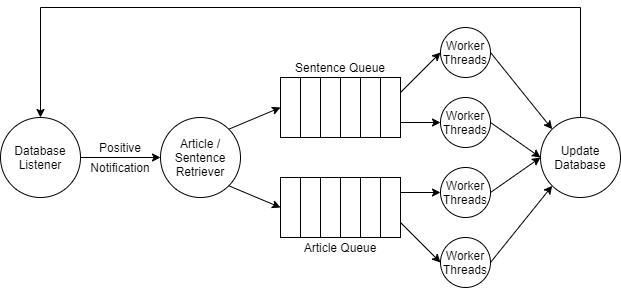
\includegraphics[width=0.5\linewidth]{images/upload/control.png}    
                \caption{Control component overview}
                \label{fig:control}
        \end{figure}
            
        Once the control component can communicate successfully with the backend components, it then setups a listener to be notified when articles are input into the system. When it receives a notification, it then splits any unfinished articles and sentences into two queues and uses multi-threading to process them. Once both queues are finished, the control component returns to listening for another notification. 
            
            \subsubsection{Listener}
            A core part of the control component is the database listener that awaits notification from the main database whenever an article or sentence is inserted into the system. This is done through a Postgres notification channel, which is set up on both the Article and Sentence tables. The control component listens to this channel, waiting for a notification to be broadcast. This prevents the component from needing to constantly poll the database for new articles and sentences.
           
            \subsubsection{Queue}
            Once a notification is received, the control component requests all unfinished articles and sentences from the database and creates a sentence and article queue. This queue is implemented using Python’s inbuilt Queue object and allows multiple worker threads to retrieve and complete tasks concurrently. 
            
            \subsubsection{Logic}
            Each worker thread uses a main sentence or article method that process an item according to its current status, see \ref{Main Database}. Each status is given a series of steps that utilize different backend components and then the database is updated. An overview of the control component’s logic can be seen in figure \ref{fig:control_logic} 
            
            \begin{figure}[!h]
                \centering
                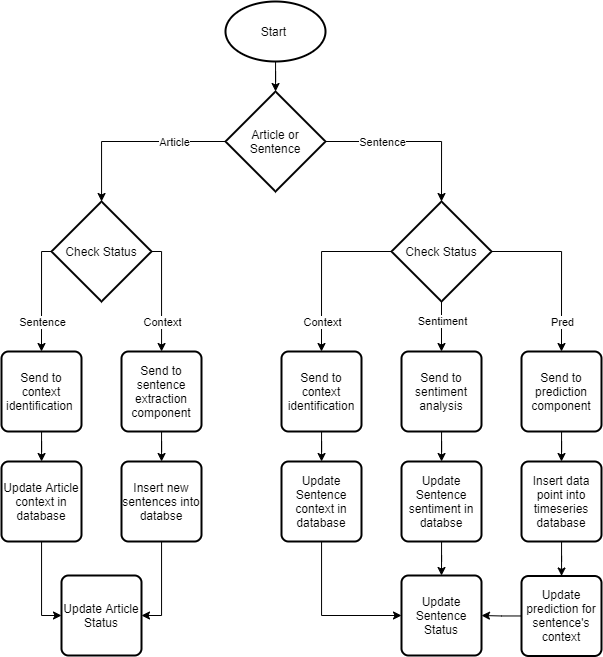
\includegraphics[width=0.4\linewidth]{images/upload/Logic Diagram.png}    
                \caption{Control component sentence and article process logic}
                \label{fig:control_logic}
            \end{figure}
            
    \section{Frontend Implementation}
    With the backend system operational, work could begin on the frontend system. An effective and user-friendly frontend system was crucial for the project and system to succeed and as such, much focus and time were spent improving and iterating on it. Django \citep{technology:Django} was the framework selected to build the frontend and its view and template building features allowed for data to be easily passed into and displayed to the website with little difficulty. 
    
        \subsection{Homepage}
        Before any stylization or features could be added to the homepage, the frontend first needed to be connected to the main database so that it could access the necessary data. Django comes connected to a Pymongo database, so it involved removing that connection and giving it the connection URL for the main database. Once the connection was successful, models were created for the Company, Sentences, Source and Tag tables in the main database. With the creation of these models, Django was able to generate its own API to the database. With the models complete, a simplistic version of the homepage was implemented to ensure that the database contents were being read correctly. This early implementation can be seen in Figure \ref{fig:Home_early}
            
        \begin{figure}[!h]
                \centering
                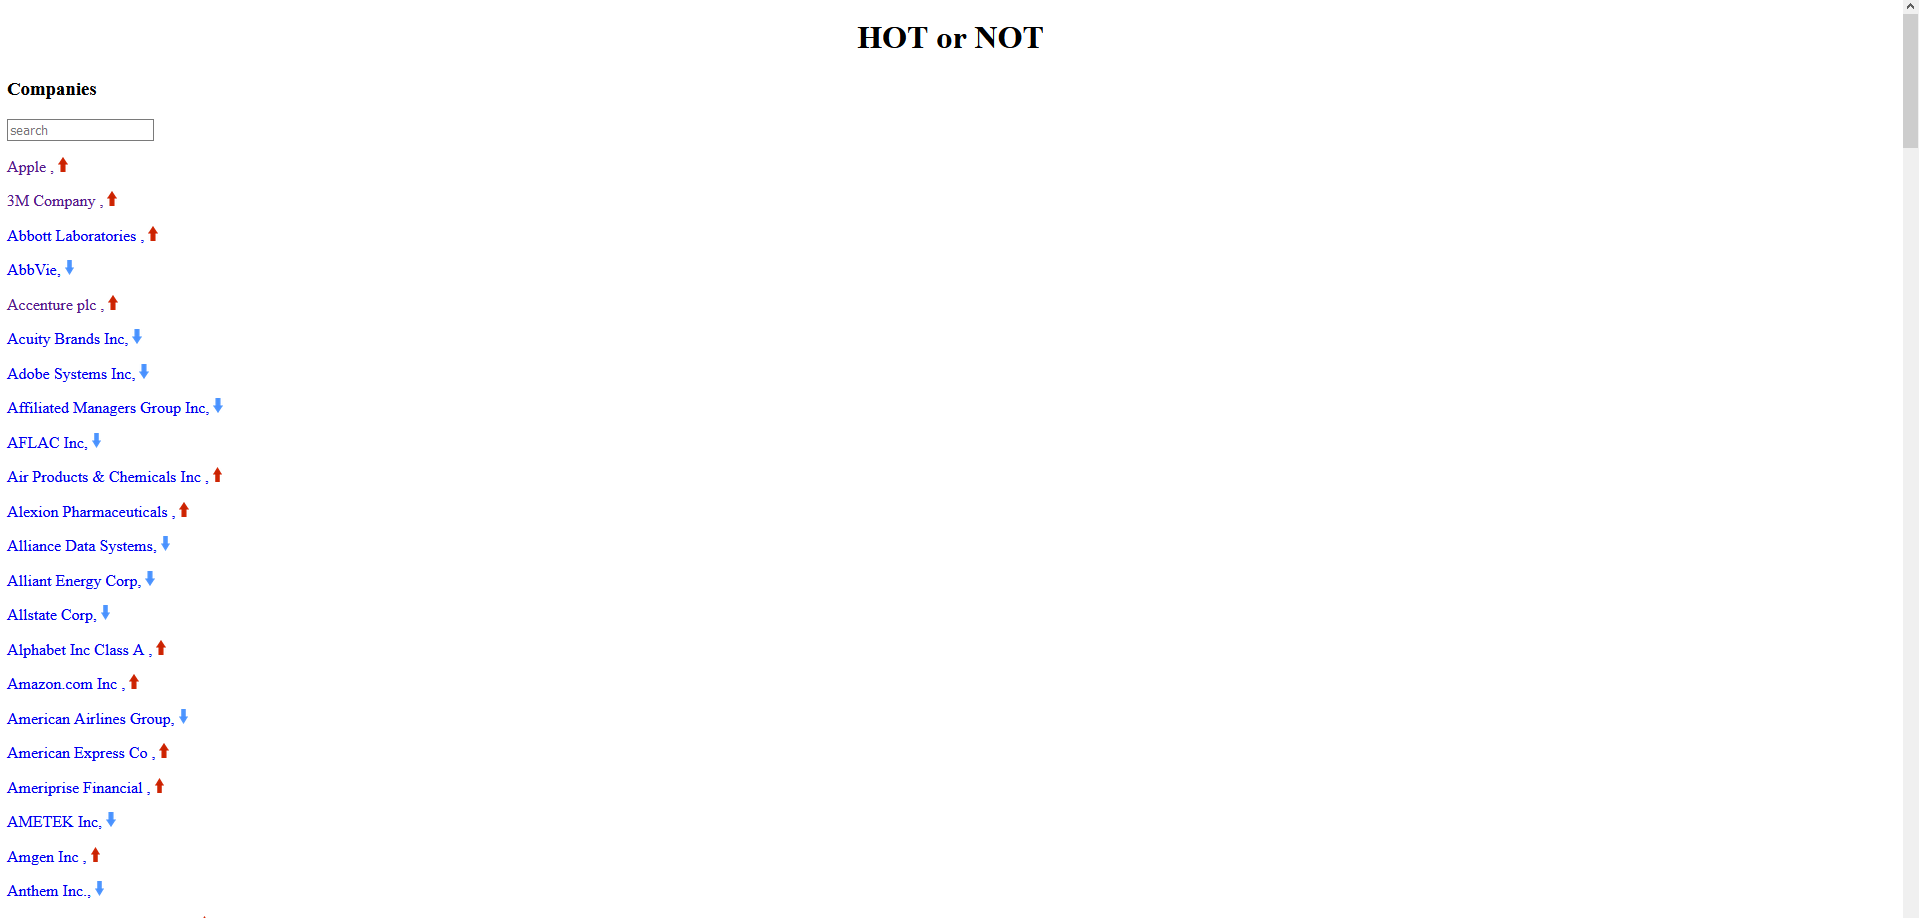
\includegraphics[width=0.5\linewidth]{images/upload/EarlyHome.png}    
                \caption{Early Implementation}
                \label{fig:Home_early}
        \end{figure}
            
        With Django fully connected to the database, the next stage implemented the designs discussed in chapter \ref{Design}
        
            \subsubsection{Company Card}
            As section \ref{Homepage} shows, each company on the homepage is given its card with styling according to its Hot or Not verdict. Initial work went into the arrangement and size of the boxes to achieve the three-column layout shown in the wireframes. With that achieved, work began on the styling and design of the company boxes. Each verdict was given its separate colour scheme and icon allowing the user to at a glance see which companies were hot and which were not. Next, the Hot or Not meter was implemented. This is based on the difference in the stock price mentioned in \ref{Verdict} and further allows the users to identify the difference between companies by seeing the degree to which they are hot or not. With the implementation of tags later in the project, the company boxes were extended to have small clickable tag buttons under the Hot or Not meter allowing the user to search and see other companies with the same tag. The company cards went through various design changes that saw the design improve through each iteration. The final implementation of the company cards can be seen in Figure \ref{fig:cards}. 
            
            \begin{figure}[!h]
            \begin{subfigure}[b]{0.5\textwidth}
                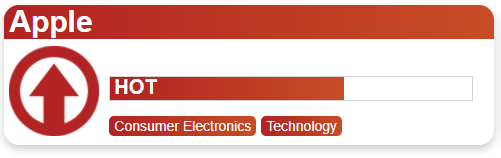
\includegraphics[width=\textwidth]{images/upload/card_hot.PNG}
                \caption{Company Card with hot status}
                \label{fig:card_hot}
            \end{subfigure}
            \hfill
            \begin{subfigure}[b]{0.5\textwidth}
                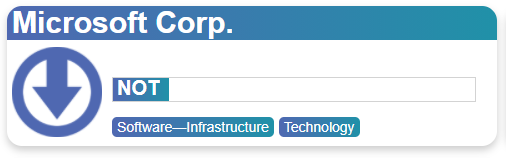
\includegraphics[width=\textwidth]{images/upload/card_not.png}
                \caption{Company Card with not status}
                \label{fig:card_not}
            \end{subfigure}
            \caption{Final implementation of the company cards}
            \label{fig:cards}
            \end{figure}
            
            \subsubsection{Search Bar}
            The search bar is perhaps the most important aspect of the homepage, as this is the main interface a potential user will use when attempting to find a company. Thanks to Djangos middleware API that is created from defined models, the frontend can easily perform queries on the main database to find any potential companies. With the implementation of tags, this search was also extended to search for companies that have similar tags to the ones that appear in the initial search. This allows not only for companies similar to the text typed by the user to appear, but also similar companies to appear.
            
            For the results of any search to be shown to the user without forcing a page to reload, AJAX was utilized to provide asynchronous updates to the homepage, changing the list of companies displayed from the database query. A sorting option was added under the search bar to allow the user to order the companies shown. The sorting options were easy to implement by simplifying the application of the sorting process for the found set of companies. The sort options given are Hot, Not, Hold, Alphabetical and stock code. Again, throughout the project's life-cycle, the search bar and the Homepage as a whole was updated and improved. The final version of the homepage can be seen in Figure\ref{fig:Home_final}
            
            \begin{figure}[!h]
                \centering
                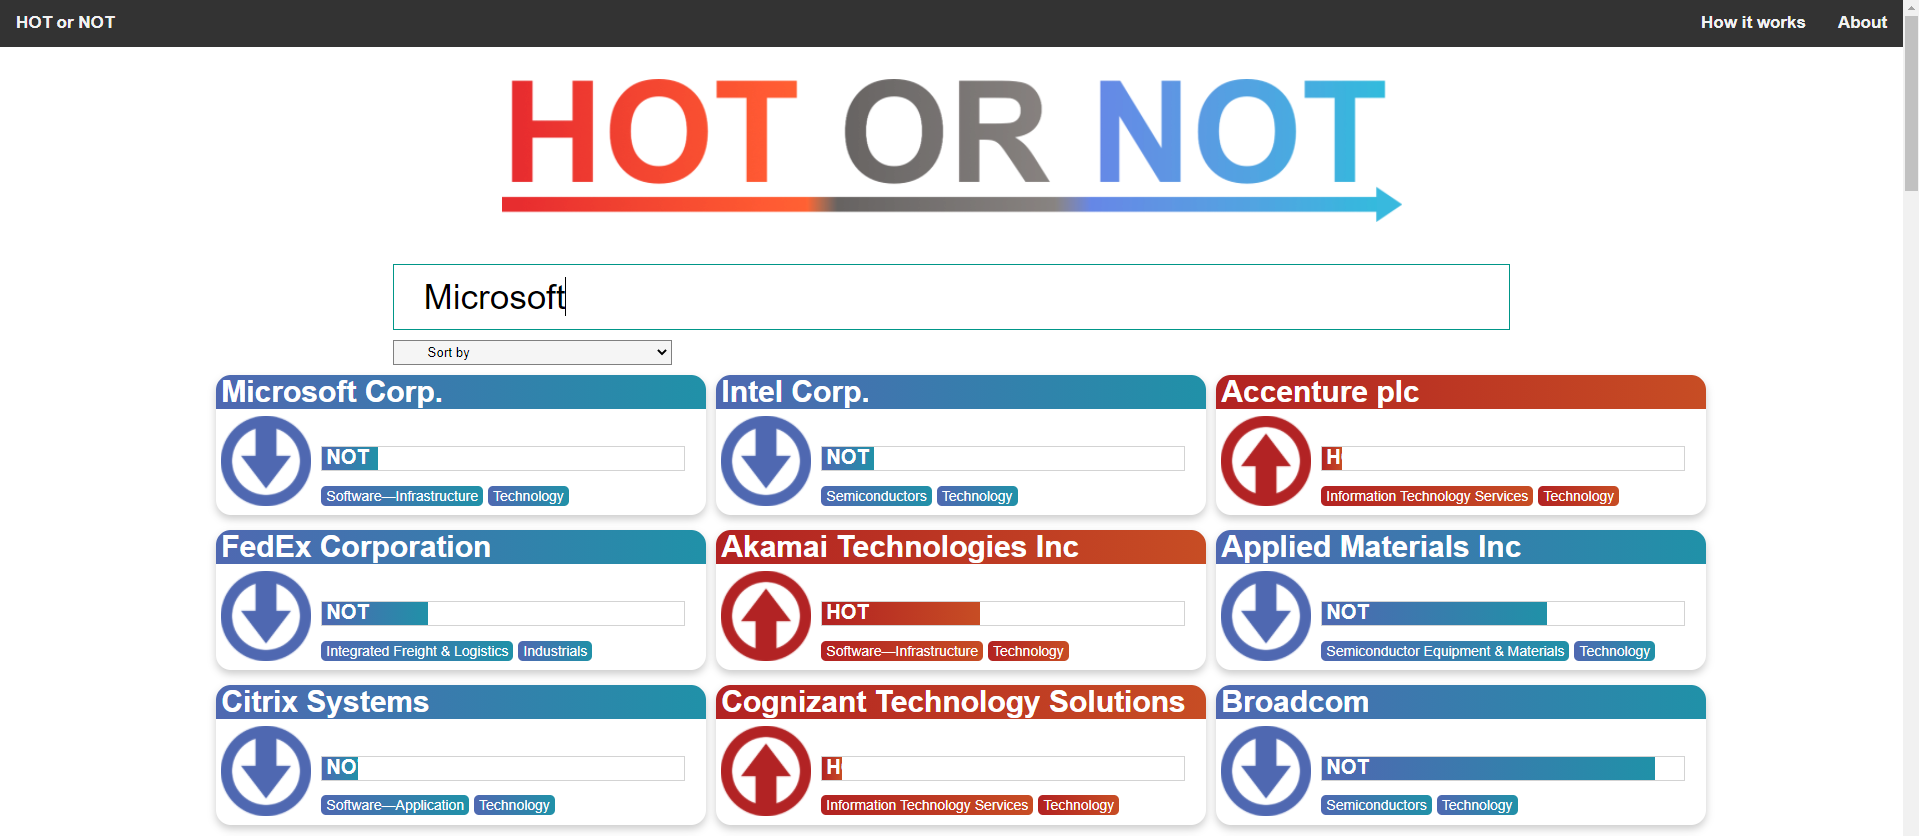
\includegraphics[width=0.9\linewidth]{images/upload/Homepage.PNG}
                \caption{Final version of the homepage}
                \label{fig:Home_final}
            \end{figure}
            
        
        \subsection{Company page}
        Once a user selects one of the company cards, they are taken to the company page. This page presents a variety of information about a given company; this information is separated into various tabs.
            
            \subsubsection{Our Predictions Tab}
            This tab stores the ready-made predictions made by the system and the verdict selection on each company is based on this. A graph of the historical stock price and predicted stock price is implemented using chartJS \citep{technology:Chartjs}, along with a chartJS extension that allows the user to drag and zoom into different areas of the chart.
            
            \subsubsection{Custom Prediction Tab}
            The custom predictions tab allows the user to create their predictions by selecting a start and end date. Firstly, to allow the user to enter the start and end date, a Django form was created that allows for safe data transfer from the webpage to the middle-ware. This form request, is processed using Ajax, sends a request to the stock prediction component containing the company stock code, along with the user defined start and end dates. The stock prediction component processes this request and returns the stock price prediction data. Thanks to Ajax, this data is then transferred to the webpage without needing to reload the page. Simply implementing chartJS and showing the custom predictions like how was done in the "Our Prediction Tab" was tried first, however there was a problem with transferring the python-generated data into the JavaScript chartJS. A small parser function was therefore created that allows the predictions to be transformed into data that works with chartJS, which is then displayed to the user. Later in the project, error handling was added to the stock prediction component and the custom prediction tab was modified to display error messages should something go wrong in the predictions. 
            
            \subsubsection{Article Snippets}
            With the majority of the core features implemented to the company page, work began on showing the article snippets for that company. A collapsible side section was added to the company page, allowing the user to view the twenty most recent sentences related to the company. To keep a consistent design throughout the webpage, the sentence boxes and section were designed to look similar to the company boxes shown on the homepage, having the same colour schemes and icons for Hot, Not and Hold sentences. Figure \ref{fig:snippets} shows the final implementation of the article snippets on the company page.
            
            \begin{figure}[!h]
                \centering
                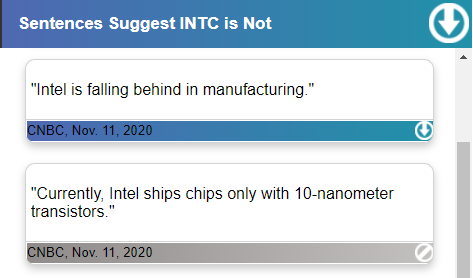
\includegraphics[width=0.5\linewidth]{images/upload/Snippets.PNG}
                \caption{Article sentence snippets}
                \label{fig:snippets}
            \end{figure}
            
            \subsubsection{Company Information Tab}
            The company information tab was originally home to basic information about the company and the different financial information on the company. However, although multiple designs and iterations to realize this tab were attempted, they did not achieve the standards of the rest of the websites and therefore it was felt that separating the tabs into "Company Profile" and "Financials" would allow for more specific designs that still remained consistent with the overall website design. The company profile and financial page all display information retrieved through the Yfiance \cite{technology:yfinance} library. The pages went through several iterations, with the final version, shown in Figure\ref{fig:info_page}, being in line with the overall style of the company page, while also displaying the information effectively. 
            
            \begin{figure}[!h]
            \begin{subfigure}[b]{0.5\textwidth}
                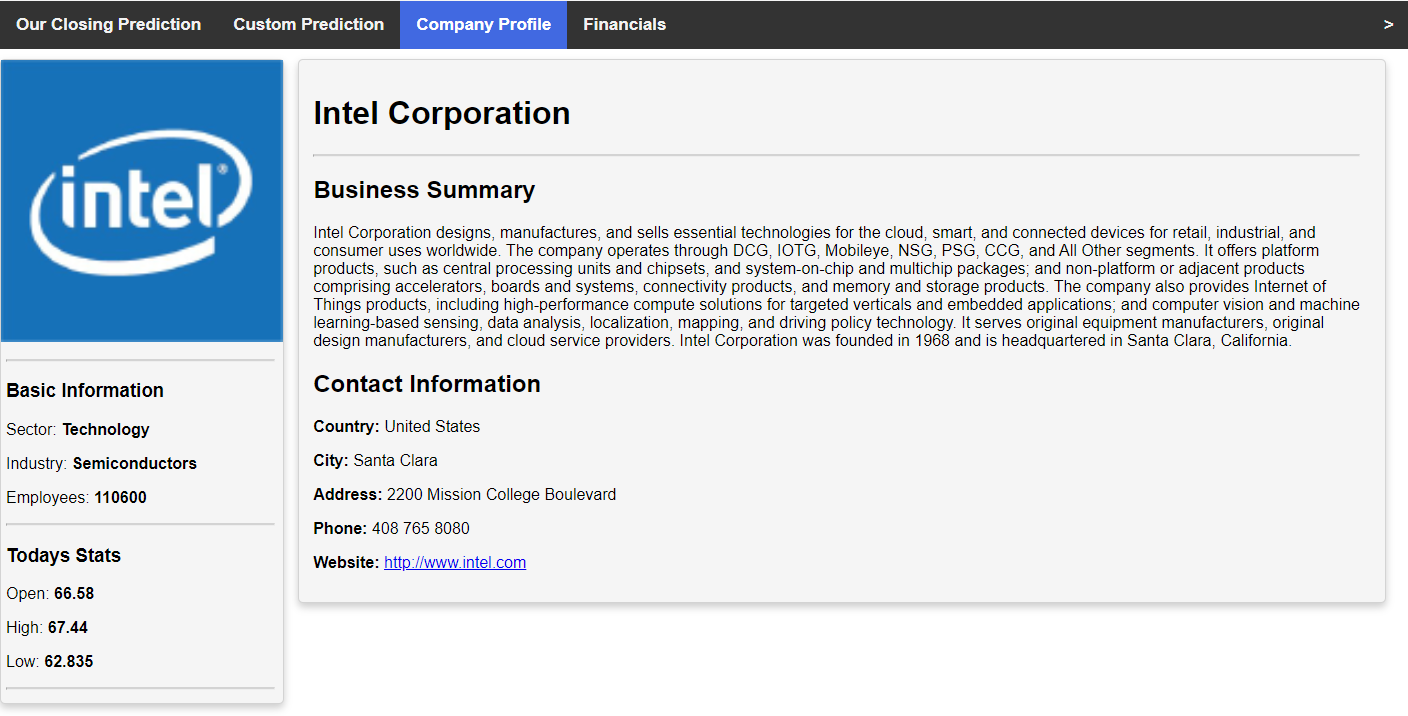
\includegraphics[width=\textwidth]{images/upload/CompanyInfo.PNG}
                \caption{Company Profile Tab}
                \label{fig:profile_tab}
            \end{subfigure}
            \hfill
            \begin{subfigure}[b]{0.5\textwidth}
                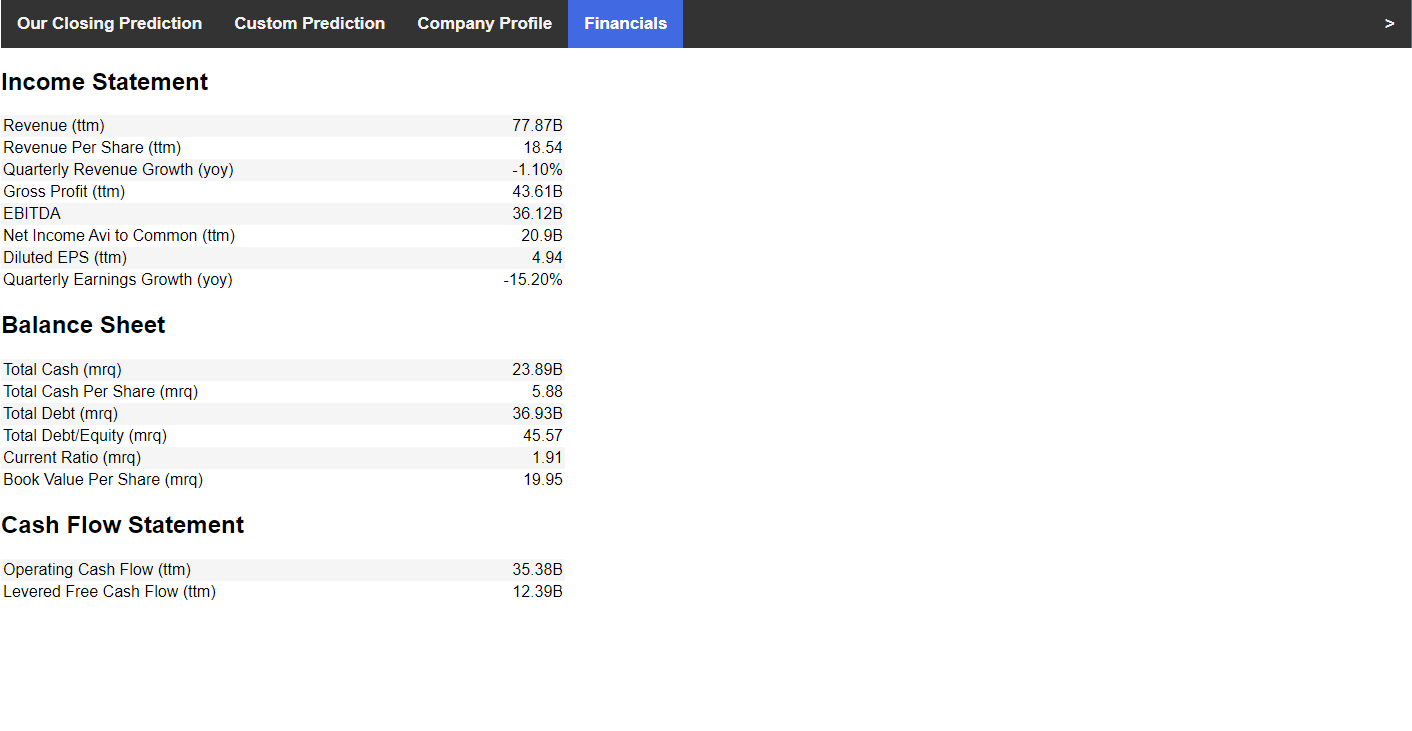
\includegraphics[width=\textwidth]{images/upload/Financial.PNG}
                \caption{Company Financial Tab}
                \label{fig:fin_tab}
            \end{subfigure}
            \caption{The company profile and financial tab of the company page}
            \label{fig:info_page}
            \end{figure}
            
            \subsubsection{AJAX} Then company page presents the user with a variety of information that both takes time to retrieve and needs constant updates, as is the case for the live stock price ticker. Therefore, it was important to shift some of the information displayed on the company page into asynchronous AJAX requests. When the company page first loads, two Ajxa requests to retrieve the financial and company information are made, which minimise some latency when loading the page. While the company page is loaded, it makes Ajax requests every five seconds to update the current stock price of the company. 
            
            \subsubsection{Overall}
            Navigating the separate tabs is done through the company page subheader that shows the company name, stock code and current stock price along with the various tabs that can be selected. The overall view of the page can be seen in Figure \ref{fig:Home_final}
            
            \begin{figure}[!h]
                \centering
                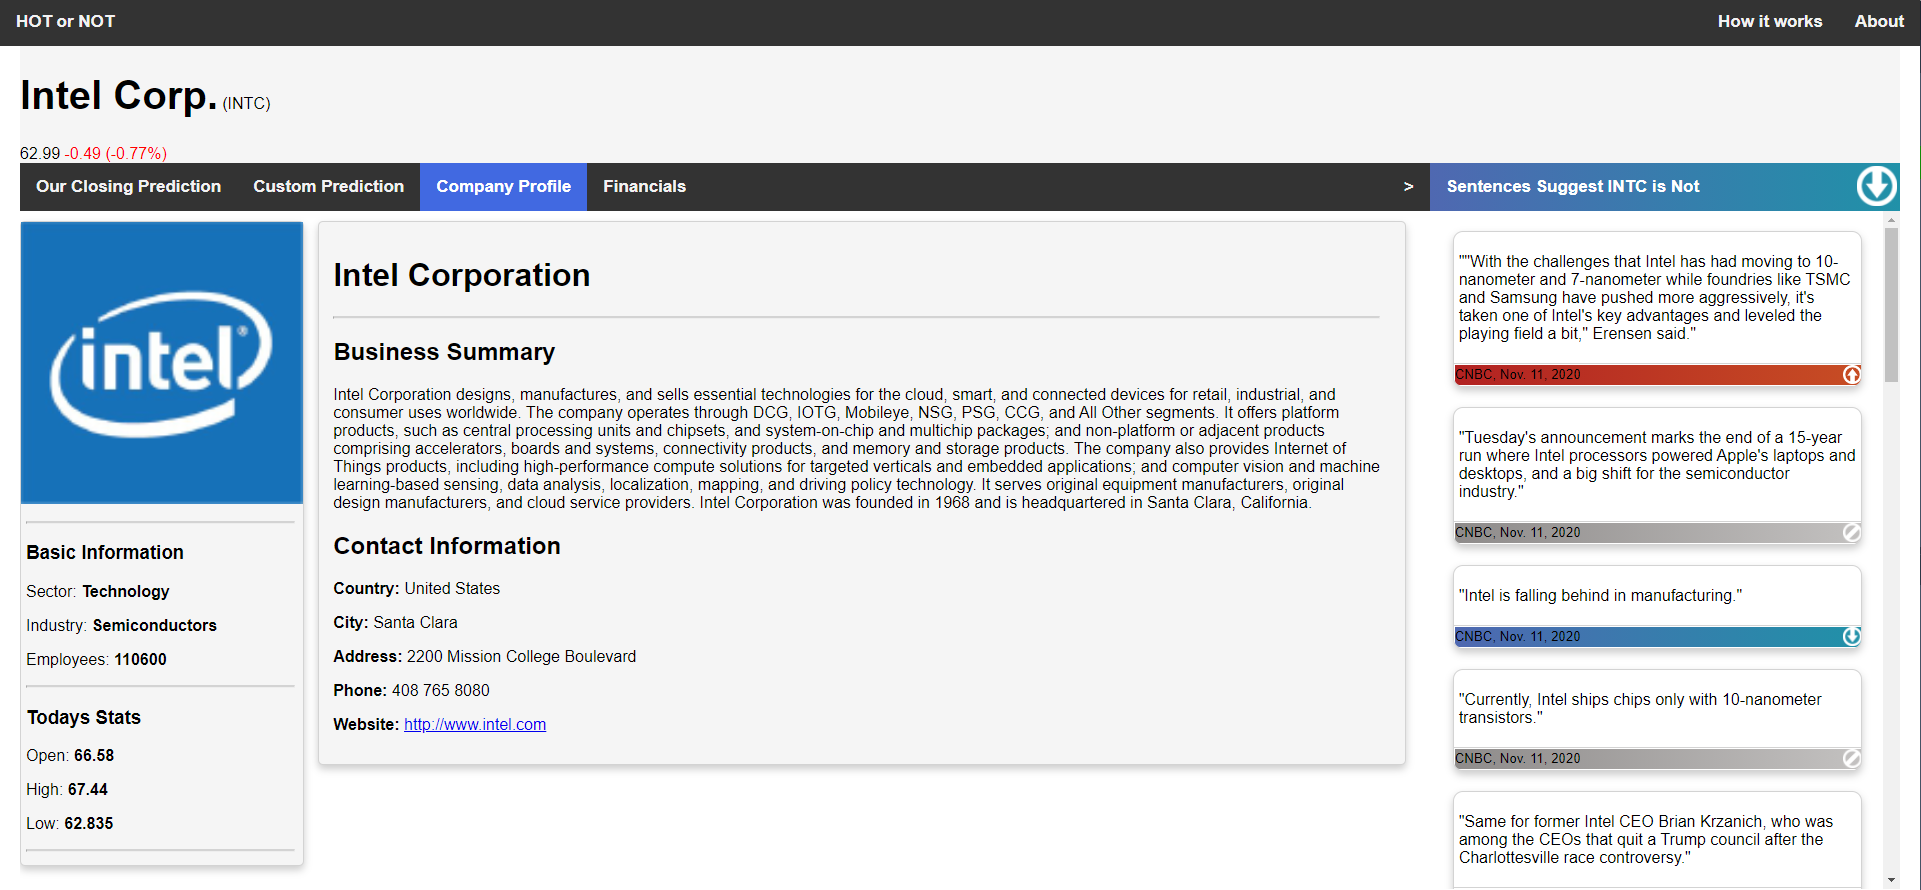
\includegraphics[width=0.9\linewidth]{images/upload/Comp_final.PNG}
                \caption{Final version of the company page}
                \label{fig:Home_final}
            \end{figure}
            
    
    \section{Containerization}
    %REDONE
    Once the system was fully working on a local level, it was important to have the project easily runnable on other machines and is a step towards to fully deploying the system. To achieve this, the various components of the system had to be implemented into containers and then connected. Docker \cite{merkel2014docker} was used to create the containers for the various components with the backend components, control component, backend API, main database, time-series database and frontend webapp all having separate containers. This meant creating requirement and Docker files across all the components, along with removing redundant data that would slow down build time. Containerizing the components went smoothly however, the main and time-series databases needed additional work. PostgreSQL and Timescale Docker base images had to be used as a starting point for the containers, with the exported SQL of the databases being imported during run time. Once the components worked individually, the next task was to tie them together using Docker Compose \citep{Jangla_2018}. Compose allows for containers to be combined into a single application increasing the ease of running the full system. A central Compose file was created detailing the Docker files for each component and their ID, run order and dependencies. Once the compose file was created, it was then a process of replacing the API call URL for each component with the new ID for the containers. 
            
    \section{Summary}
    This chapter details the steps, challenges and solutions in implementing the \textit{Hot or Not} system. The chapter highlights the software engineering practices used throughout the project and the benefit they had on the projects development. A description and justification of the technologies and steps taken to implement the backend, database and frontend systems along with how those separate components were integrated to create the overall working system. More information on the final deliverable can be found in Appendix \ref{Ap: Final Deliverable}.
    
    
    
% List requiremts
% Ret   Test    Pass or Fail

% Test, what test / performance lead you to consider  it complete
% Logical test

% Summary, key findings

% Only four decimal points

% Complete Requirement validation

% Add in unit testing

%BACKGROUND
    
    %WHAT DOING (QUESTION)
    
    %HOW GOING TO DO - data set
    
    %TELL EXPECTATIONS
    
    %DESCRIBE THING (TABLE)
    
    %MAKE OBSERVATIONS FROM TABLE
    
    %DRAW CONCLUSION
    
    %SAY WHAT IT MEANS ABOUT SSYTEM
    
    
\chapter{Evaluation}
\label{Evaluation}
Evaluating and improving the overall system was a main focus of the project, as it was not only important to have accurate predictions shown to users but also important to document how those improvements were made.

    \section{Correctness Testing}
    
        \subsection{Requirement Validation}
        
        \subsubsection{Backend Requirements } \phantom{}
        \begin{table}[h]
            \begin{tabular}{|l|l|l|}
                \hline
                Requirement           & Test & Pass or Fail \\ \hline
                \#1: Article Gatherer      & \begin{tabular}[c]{@{}l@{}} Met by News Crawler component \\~ \end{tabular}   & PASS            \\ \hline
                \#2: Database              & \begin{tabular}[c]{@{}l@{}} Met by main database and \\ time-series database \end{tabular}   & PASS            \\ \hline
                \#3: Context Identification & \begin{tabular}[c]{@{}l@{}} Met by context analysis component \\~ \end{tabular}    & PASS            \\ \hline
                \#4: Sentence Extraction   & \begin{tabular}[c]{@{}l@{}} Met by sentence extraction component \\~ \end{tabular}    & PASS            \\ \hline
                \#5: Sentiment Analysis    & \begin{tabular}[c]{@{}l@{}} Met by sentiment analysis component \\~ \end{tabular}    & PASS            \\ \hline
                \#6: Stock prediction      & \begin{tabular}[c]{@{}l@{}} Met by stock prediction component \\~ \end{tabular}    & PASS            \\ \hline
                \#7: Accurate Context Analysis & \begin{tabular}[c]{@{}l@{}} Component performance evaluated and \\ improved in section \ref{eval:context} \end{tabular}    & PASS            \\ \hline
                \#8: Accurate Sentiment Analysis & \begin{tabular}[c]{@{}l@{}} Component performance evaluated and \\ improved in section \ref{eval:sentiment} \end{tabular}   & PASS            \\ \hline
                \#9: Accurate Prediction &  \begin{tabular}[c]{@{}l@{}} Component performance evaluated and \\ improved in section \ref{eval:prediction} \end{tabular}    & PASS             \\ \hline
                \#10: Variety of companies & \begin{tabular}[c]{@{}l@{}} Met by databases storing \\ multiple companies in system\end{tabular}   & PASS            \\ \hline
                \#11: Prediction Options & \begin{tabular}[c]{@{}l@{}} Met by custom prediction option in \\ webapp \end{tabular}   & PASS            \\ \hline
                \#12: Deployed and Accessible & \begin{tabular}[c]{@{}l@{}} Met by webapp being accessible \\  by users \end{tabular}   & FAIL            \\
                \hline
            \end{tabular}
        \end{table}
        \newline
        \subsubsection{Frontend Requirements}  \phantom{}
        
        \begin{table}[h]
            \begin{tabular}{|l|l|l|}
                \hline
                Requirement                 & Test & Pass or Fail \\ \hline
                \#13: Home page             & \begin{tabular}[c]{@{}l@{}} Met by homepage of webapp \\ \end{tabular}    & PASS            \\ \hline
                \#14: Company page          & \begin{tabular}[c]{@{}l@{}} Met by company page of webapp \end{tabular}   & PASS            \\ \hline
                \#15: Search bar            & \begin{tabular}[c]{@{}l@{}} Met by search bar on home \\ page of webapp \end{tabular}   & PASS            \\ \hline
                \#16: Filters and tags      & \begin{tabular}[c]{@{}l@{}} Met by tag table in system and \\ filter option on webapp \end{tabular}  & PASS            \\ \hline
                \#17: prediction results    & \begin{tabular}[c]{@{}l@{}} Met by prediction graph on \\ company page \end{tabular}   & PASS            \\ \hline
                \#18: stock graph           & \begin{tabular}[c]{@{}l@{}} Met by stock graph on company \\ page \end{tabular}   & PASS            \\ \hline
                \#19: related companies     & \begin{tabular}[c]{@{}l@{}} Met by search results showing \\ similar companies \end{tabular}   & PASS            \\ \hline
                \#20: website design        & \begin{tabular}[c]{@{}l@{}} Met by component achieving acceptable  \\ SUS score in section \ref{eval:user_study}  \end{tabular}   & PASS            \\ \hline
                \#21: additional information & \begin{tabular}[c]{@{}l@{}} Met by company profile and financials \\ tab on company page \end{tabular}    & PASS            \\ \hline
                \#22: Personalisation       & \begin{tabular}[c]{@{}l@{}} Met by ability to create account \\ and tailor the website to needs \end{tabular}   & FAIL            \\ \hline
                \#23: Article snippets      & \begin{tabular}[c]{@{}l@{}} Met by sentence side bar on \\ company page \end{tabular}   & PASS            \\ \hline
            \end{tabular}
        \end{table}
        
        \subsection{Unit Test}
        In order to evaluate the Backend API, a series of unit tests were created. These unit tests operate on the source, article, sentence and company API calls. Four unit test classes were created relating to Source, Article, Sentence and Company with each having testing API calls that inserted, modified, retrieved and deleted data. This ensured that data was being inputted and modified correctly whenever a change was made to the Backend API. 
        
    
    \section{Backend Evaluation}
    The backend system contains multiple machine learning models that assisted in the processing of articles and sentences. Evaluating the system was necessary to improve the overall prediction performance and effectiveness of the system. The three major components that impact final prediction performance are the context analysis component, sentiment analysis component and stock prediction component. To discover bottlenecks in the overall system and find ways to improve the performance it was critical that these three components be evaluated. 
    
        \subsection{Context Analysis}
        \label{eval:context}
        %Background
        The context analysis component is an important first step in the system as it is used to understand what companies are being discussed in a given article or sentence. This is done through a named entity recognition model provided by Spacy \citep{technology:Spacy} that identifies and labels entities in a given text. These entities can be given various labels however the ones we are concerned with are Organisation, Person and Location. 
        
        %WHAT
        To access the performance of the component we will first evaluate the performance of the current Spacy model and compare it to that model of another technology, that being Stanza \citep{technology:Stanza}. %HOW
        To do this, we will use an annotated data set containing over 47,000 sentences sourced from Kaggle. Both models will be used to analyze each sentence in the dataset and compare the potential entities found to the actual entities in the dataset. Recording the results for each model and entity type will allow us to compare the model's performances.
        %EXPECTIATION
        Since Stanza contains a more modern and advanced named entity recognition model we should expect to see a performance increase with this model.
        
        %DESCRIBE TABLE
        Tables \ref{sub:spacy} and \ref{sub:stanza} show the performance results for each model, with each row being a different entity type and each column being a different performance metric to create a confusion matrix. 
        %Observation from table
        Looking at Spacy's results in \ref{sub:spacy} and comparing them to Stanza results in \ref{sub:stanza} we can see that Stanza's overall performance is better, scoring marginally higher than the Spacy model in all four metrics.
        
        %Draw conclusion / what it means
        Overall we can see that Stanza provides a more effective NER model than the one previously being used through Spacy. This means that the context analysis component is more effective using the Stanza model and was duly modified to do so.
        
        \begin{table}[h]
            \centering
            \begin{subtable}{\textwidth}
                \centering
                \begin{tabular}{|l|l|l|l|l|} 
                \hline
                \textbf{Entity Type} & \textbf{Accuracy}                           & \textbf{Precision}                          & \textbf{Recall}                             & \textbf{F1}                                  \\ 
                \hline
                Organisation         & {0.725973} & {0.646951} & {0.273625} & {0.38459}   \\ 
                \hline
                Person               & {0.818419} & {0.710441} & {0.273704} & {0.395167}  \\ 
                \hline
                Location             & {0.768405} & {0.805118} & {0.747453} & {0.775215}  \\ 
                \hline
                Other                & {0.513416} & {0.366572} & {0.479684} & {0.415568}  \\ 
                \hline
                \textbf{Overall}     & {0.70153}  & {0.62525}  & {0.4737}   & {0.53902}   \\
                \hline
                \end{tabular}
                \smallskip
                \caption{Spacy NER confusion matrix} \label{sub:spacy}
            \end{subtable}
            \bigskip
            \begin{subtable}{\textwidth}
                \centering
                \begin{tabular}{|l|l|l|l|l|} 
                \hline
                \textbf{Entity Type} & \textbf{Accuracy}                                                              & \textbf{Precision}                                                             & \textbf{Recall}                                                                & \textbf{F1}                                                                     \\ 
                \hline
                Organisation         & {}{0.7600}  & {0.7248}                                    & {0.2705}                                    & {0.3940}                                     \\ 
                \hline
                Person               & {0.8509}                                    & {0.7513}                                    & {0.2907}                                    & {}{0.4199}  \\ 
                \hline
                Location             & {}{0.7802} & {}{0.7937} & {0.7580}                                    & {0.7755}                                     \\ 
                \hline
                Other                & {0.5072}                                     & {0.3606}                                    & {}{0.4839} & {0.4133}                                      \\ 
                \hline
                \textbf{Overall}     & {0.7171}                                    & {0.6343}                                    & {0.4808}                                    & {0.5470}                                     \\
                \hline
                \end{tabular}
                \caption{Stanza NER confusion matrix} \label{sub:stanza}
            \end{subtable}
            \smallskip
            \caption{NER model performances} \label{tab:eval_NER}
        \end{table}
        
        In order to evaluate the true performance gain, provided by the Stanza model, we need to access the performance increase of the overall system. To do this, we devised an end to end test of the entire system to compare the prediction performance when using the Spacy NER model to the prediction performance when using the Stanza NER model.
                
        The prediction performance is measured using news data gathered from the news crawler between November 11th 2020 to December 15th 2020, ensuring that both of the NER models use the same data set and that the evaluation is fair. The Mean Squared Error and the median absolute error are calculated for each company for a given time frame and the results shown on the Table show the average across all companies. Since we previously saw superior performance with the Stanza model, we expected to see a similar result provided to the overall system.
                
        Table \ref{Table: NER_Performance} shows the Mean Squared Error and median absolute error for each model in a 1 day to 30-day time frame. Table \ref{Table: NER_Performance} shows a small yet noticeable and consistent performance increase across all time frames when the Stanza model was used. This shows that the positive impact on performance that the Stanza model had on the component also had a positive impact on the performance of the overall system. 
                
        \begin{table}[h]
            \centering
            \begin{tabular}{|l|l|l|l|l|l|l|}
            \multicolumn{3}{l}{Mean Squared Error}                                                                                                & \multicolumn{1}{l}{} & \multicolumn{3}{l}{Median Absolute Error}                                                       \\ 
            \cline{1-3}\cline{5-7}
            Time Frame & Spacy                                                                        & Stanza                                    &                      & Time Frame & Spacy                                   & Stanza                                   \\ 
            \cline{1-3}\cline{5-7}
            1 day      & {50.86}                                     & {49.57}  &                      & 1 day      & {3.42} & {3.38}  \\ 
            \cline{1-3}\cline{5-7}
            2 days     & {}{93.1}   & {91.5}   &                      & 2 days     & {4.03} & {3.97}  \\ 
            \cline{1-3}\cline{5-7}
            5 days     & {}{123.48} & {122.92} &                      & 5 days     & {4.72} & {4.63}  \\ 
            \cline{1-3}\cline{5-7}
            10 days    & {141.06}                                    & {136.68} &                      & 10 days    & {5.37} & {5.29}  \\ 
            \cline{1-3}\cline{5-7}
            15 days    & {}{160.25} & {158.4}  &                      & 15 days    & {5.55} & {5.47}  \\ 
            \cline{1-3}\cline{5-7}
            30 days    & {}{209.92} & {207.41} &                      & 30 days    & {6.36} & {6.28}  \\
            \cline{1-3}\cline{5-7}
            \end{tabular}
            \bigskip
            \caption{Prediction performance comparisons between Spacy and Stanza}
            \label{Table: NER_Performance}
        \end{table}
        
        \subsection{Sentiment Analysis}
        \label{eval:sentiment}
        The sentiment analysis component is used to analyze the sentiment expressed in sentences in the system. This sentiment goes on to found the basis of predictions made in the stock prediction component and therefore is a critical component in the overall system. Initially, the sentiment was analyzed using VADER sentiment \citep{Technology:Vader} however other technologies exist that could provide better results.
        
        Therefore, to evaluate the sentiment analysis component, we will compare the performance of the VADER sentiment model to two other technologies. The first technology we looked at was the Natural Language Toolkit \citep{Technology:NLTK}, or NLTK, which is an extensive Python library that has a whole host of language processing models and features, one of which is sentiment analysis. The second technology evaluated was Textblob \citep{technology:Textblob}, an extension to NLTK that provides easier and more simplistic APIs to make full use of NLTK's features.
      
        To access the performance of each technology, an annotated data set comprising 4,846 sentences collected from financial news streams was sourced from Kaggle. Each sentence in the data set is labelled -1, 0 or 1 meaning negative sentiment, neutral sentiment or positive sentiment. Each technology analyzed all the sentences in the set and compared its result to the actual ones in the dataset. Keeping track of the correct and incorrect scores allows us to calculate the precision, recall and F1 score for each technology. Since NLTK is a more established technology, we expect to see some improvement between that and VADER sentiment and perhaps even more improvement with Textblob, since it is an extension to NLTK. 
        
        \begin{table}[h]
        \centering
            \begin{subtable}{\textwidth}
                \centering
                \begin{tabular}{|l|l|l|l|} 
                \hline
                         & Precision                                   & Recall                                      & F1 Score                                     \\ 
                \hline
                Positive & {0.4732} & {0.7116} & {0.5684}  \\ 
                \hline
                Negative & {0.5462} & {0.3129} & {0.3979}  \\ 
                \hline
                Neutral  & {0.7996} & {0.6804} & {0.7352}  \\
                \hline
                \end{tabular}
                \smallskip
                \caption{VADER sentiment confusion Matrix} \label{sub:sent_vader}
            \end{subtable}
            
            \bigskip
            
            \begin{subtable}{\textwidth}
                \centering
                \begin{tabular}{|l|l|l|l|} 
                \hline
                         & Precision                                                                      & Recall                                                                         & F1 Score                                                                        \\ 
                \hline
                Positive & {}{0.4741} & {0.7117}                                    & {}{0.5691}  \\ 
                \hline
                Negative & {}{0.4741} & {}{0.3113} & {}{0.3962}  \\ 
                \hline
                Neutral  & {}{0.8}      & {0.6821}                                    & {}{0.7364}  \\
                \hline
                \end{tabular}
                \smallskip
                \caption{NLTK confusion Matrix} \label{sub:sent_NLTK}
            \end{subtable}
            
            \bigskip
            
            \begin{subtable}{\textwidth}
                \centering
                \begin{tabular}{|l|l|l|l|} 
                \hline
                         & Precision                                   & Recall                                                                         & F1 Score                                     \\ 
                \hline
                Positive & {0.6577} & {0.4285}                                    & {0.5189}   \\ 
                \hline
                Negative & {0.5550} & {}{0.3841} & {0.4540}  \\ 
                \hline
                Neutral  & {0.7443}  & {0.9153}                                    & {0.821}     \\
                \hline
                \end{tabular}
                \smallskip
                \caption{Textblob confusion Matrix} \label{sub:sent_Textblob}
            \end{subtable}
            
        \caption{Sentiment analysis performance}
        \end{table}
        
        Tables \ref{sub:sent_vader}, \ref{sub:sent_NLTK} and \ref{sub:sent_Textblob} show the results for each technology, with the results being separated into metrics for positive, negative and neutral sentences. Comparing NLTK in Table \ref{sub:sent_NLTK} to VADER sentiment in Table \ref{sub:sent_vader} we can see that NLTK performs better with neutral and positive sentences, however recorded a decrease in performance for negative sentences. Textblob's F1 score in Table \ref{sub:sent_Textblob} shows that it performed better than both NLTK and VADER sentiment for negative and neutral sentences, but performed slightly worse for positive sentences. Overall, NLTK and Textblob provided better performances than the VADER sentiment model with Textblob having the best performance overall. It was therefore decided that the sentiment analysis component would use the Textblob sentiment model.
        
        Similar to what was done with the context analysis component we needed to evaluate the overall performance increase to the system through end-to-end testing. Again, this was done using news data gathered from the news crawler between November 11th 2020 to December 15th 2020 and comparing the prediction performances to the old system which used VADER sentiment to the new system which uses Textblob.
        
        Looking at Table \ref{Table: sent_Performance} again, similar to the performance increase in the context analysis component, we see a small, yet noticeable performance increase across all time frames suggesting that the improvements to the sentiment analysis component have had a positive impact on the overall performance of the system. 
        
        \begin{table}[h]
            \centering
            \begin{tabular}{|l|l|l|l|l|l|l|}
            \multicolumn{3}{l}{Mean Squared Error}                             & \multicolumn{1}{l}{} & \multicolumn{3}{l}{Median Absolute Error}  \\ 
            \cline{1-3}\cline{5-7}
            Time Frame & VADER sentiment                                     & Text Blob &                      & Time Frame & VADER sentiment & Text Blob             \\ 
            \cline{1-3}\cline{5-7}
            1 day      & {51.44}  & 50.86     &                      & 1 day      & 3.52  & 3.42                  \\ 
            \cline{1-3}\cline{5-7}
            2 days     & {99.8}   & 93.1      &                      & 2 days     & 4.23  & 4.03                  \\ 
            \cline{1-3}\cline{5-7}
            5 days     & {134.05} & 123.48    &                      & 5 days     & 4.95  & 4.72                  \\ 
            \cline{1-3}\cline{5-7}
            10 days    & {159.97} & 141.06    &                      & 10 days    & 5.79  & 5.37                  \\ 
            \cline{1-3}\cline{5-7}
            15 days    & {190.01} & 160.25    &                      & 15 days    & 6.61  & 5.55                  \\ 
            \cline{1-3}\cline{5-7}
            30 days    & {242.8}  & 209.92    &                      & 30 days    & 6.87  & 6.36                  \\
            \cline{1-3}\cline{5-7}
            \end{tabular}
            \bigskip
            \caption{Prediction performance comparisons between VADER sentiment and Text Blob}
            \label{Table: sent_Performance}
        \end{table}
        
        \subsection{Stock Prediction Component}
        \label{eval:prediction}
        %Background
        The stock prediction component is what makes the final prediction for companies in the system and is the culmination of all the previous components. The component contains two models: the sentiment model, used to predict missing and future sentiment, and the stock prediction model, used to predict a company's stock price at a given time. Since the component was built using Sklearn \citep{technology:Scikit-learn}, which comes packaged with multiple different models, it was simple to replace models for trials.
        
            \subsubsection{Sentiment Model} We will first evaluate the sentiment model by looking at the different possible models that could improve the overall prediction performance and compare them to one another. To do this, we will compare the prediction performance results in a one-day time frame for different models, using the articles crawled between November 11th 2020 to December 15th 2020 as training data. Table \ref{Table: pred_sent_model} shows the three most effective models tested; Support vector machines (SVM), Bayesian regression and Bayesian regression with a Scalar to the data applied along with their associated MSE and MAE scores. Looking at the Table it would suggest that a Bayesian model is more effective along with a marginal performance when a scalar is applied to the training data.
            
            \begin{table}[h]
            \centering
            \begin{tabular}{|l|l|l|l|} 
            \cline{2-4}
            \multicolumn{1}{l|}{} & \textbf{SVM} & \textbf{Bayesian} & \textbf{Bayesian + Scalar}  \\ 
            \hline
            MSE                   & 50.86                      & 49.78             & 49.9                        \\ 
            \hline
            MAE                   & 3.42                       & 3.405             & 3.3                         \\
            \hline
            \end{tabular}
            \caption{Comparison between different models in a one day time-frame}
            \bigskip
            \label{Table: pred_sent_model}
            \end{table}
            
            Since Table \ref{Table: pred_sent_model} suggested an improvement with the Bayesian model with a scalar over the Support Vector Machine approach originally used, a more extensive evaluation was performed. Using the November 11th 2020 to December 15th 2020 article data the Mean Squared Error and mean absolute error scores of the SVM and Bayesian and Scalar model were calculated for 1 day to 30-day time frame. Table \ref{Table: pred_sent_final} shows the results of the test performed and suggests an increase in performance using the Bayesian Model with a scalar across all time frames. 
            
            \begin{table}[h]
            \caption{Performance comparison between SVM sentiment model and Bayesian model with a scalar}
            \label{Table: pred_sent_final}
            \centering
            \begin{tabular}{|l|l|l|l|l|l|l|}
            \multicolumn{3}{l}{Mean Squared Error}                                                                         & \multicolumn{1}{l}{} & \multicolumn{3}{l}{Median Absolute Error}  \\ 
            \cline{1-3}\cline{5-7}
            Time Frame                                                                           & SVM    & Bayesian + Scalar &                      & Time Frame & SVM  & Bayesian + Scalar         \\ 
            \cline{1-3}\cline{5-7}
            {1 day}                                             & 50.86  & 49.9           &                      & 1 day      & 3.42 & 3.38                   \\ 
            \cline{1-3}\cline{5-7}
            {2 days}                                            & 93.1   & 91.6           &                      & 2 days     & 4.03 & 3.96                   \\ 
            \cline{1-3}\cline{5-7}
            {5 days}                                            & 123.48 & 121.90         &                      & 5 days     & 4.72 & 4.67                   \\ 
            \cline{1-3}\cline{5-7}
            {10 days} & 141.06 & 138.76         &                      & 10 days    & 5.37 & 5.31                   \\ 
            \cline{1-3}\cline{5-7}
            15 days                                                                              & 160.25 & 158.02         &                      & 15 days    & 5.55 & 5.47                   \\ 
            \cline{1-3}\cline{5-7}
            30 days                                                                              & 209.92 & 207.56         &                      & 30 days    & 6.36 & 6.31                   \\
            \cline{1-3}\cline{5-7}
            \end{tabular}
            \end{table}
        
            
        \subsubsection{Stock Prediction Model}
        The final model to be evaluated in the system was the stock prediction model, which is used to predict the future prices of a given stock using the sentiment data collected. This prediction is then used to determine the overall verdict of a company, which is then displayed to the user.
        
        To evaluate the prediction model, we compared the effectiveness of the current Support Vector Machines model to other potentially effective models. We used sentiment data scraped by the news crawler between November 11th 2020 to December 15th 2020 to train the different models, then compared how they performed in 1 day to 30-day intervals into the future per company and calculated the averages  to create an overall score for each company. The two other models evaluated were a Decision Tree regression model and a Random Forest regression model. 
        
        Table \ref{Table: pred_MSE} shows the Mean Squared Error (MSE) for each model tested and each time frame into the future. \ref{Table: pred_MAE} shows the Mean Absolute Error (MAE) for each model tested for each time frame into the future. Table \ref{Table: pred_MSE} and Table \ref{Table: pred_MAE} both show a considerable performance increase from an SVM model to the Decision Tree or Random Forest across all time frames, however, SVM does show better MSE results for the 30-day time frames.
        
        Overall, we can see that there was a considerable performance increase when using a Decision Tree or Random Forest model over an SVM one. Therefore, it proved that switching to one of these models would also be beneficial for the system as a whole. The Random Forest regressor was selected to be implemented over the Decision Tree model for multiple reasons. Firstly, Random Forest proved to be more effective in the long term and does not overfit the data as the Decision Tree Model does.
        
        \begin{table}[h]
            
            \begin{subtable}{\linewidth}
            \centering
            \begin{tabular}{|l|l|l|l|}
            \multicolumn{4}{l}{Mean Squared Error}                                                                                                                                                    \\ 
            \hline
            Time Frame & SVM                                       & Decision Trees                            & Random Forest                                                                        \\ 
            \hline
            1 day      & 50.86                                     & 23.91                                     & 27.3                                                                                 \\ 
            \hline
            2 days     & {93.1}   & {63.42}  & {72.88}                                             \\ 
            \hline
            5 days     & {123.48} & {113.7}  & {103.49}                                            \\ 
            \hline
            10 days    & {141.06} & {135.38} & {126.08}  \\ 
            \hline
            15 days    & {160.25} & {146.12} & {138.96}                                            \\ 
            \hline
            30 days    & {209.92} & {257.5}  & {253.6}                                             \\
            \hline
            \end{tabular}
            \bigskip
            \caption{Mean Squared Error performance of the SVM, Decision Tree Regressor and Random Forest Regressor models for the stock prediction component}
            \label{Table: pred_MSE}
            \end{subtable}
            
            \bigskip
            
            \begin{subtable}{\linewidth}
            \centering
            \begin{tabular}{|l|l|l|l|}
            \multicolumn{4}{l}{Mean Absolute Error}                                                                                                                                             \\ 
            \hline
            Time Frame & SVM                                     & Decision Trees                          & Random Forest                                                                      \\ 
            \hline
            1 day      & {3.38} & {2.41} & {2.16}                                            \\ 
            \hline
            2 days     & {3.96} & {3.03} & {2.89}                                            \\ 
            \hline
            5 days     & {4.67} & {4.06} & {3.82}                                            \\ 
            \hline
            10 days    & 5.31                                    & 4.69                                    & {4.44}                                            \\ 
            \hline
            15 days    & 5.47                                    & 4.86                                    & 4.63                                                                               \\ 
            \hline
            30 days    & 6.31                                    & 5.84                                    & 5.71                                                                               \\
            \hline
            \end{tabular}
            \bigskip
            \caption{Mean Absolute Error performance of the SVM, Decision Tree Regressor and Random Forest Regressor models for the stock prediction component}
            \label{Table: pred_MAE}
            \end{subtable}
        
        \caption{Mean Squared Error and Median Absolute Error for stock prediction models}
        \label{Table: pred_final}
        \end{table}
    
    %BACKGROUND
    
    %WHAT DOING (QUESTION)
    
    %HOW GOING TO DO - data set
    
    %TELL EXPECTATIONS
    
    %DESCRIBE THING (TABLE)
    
    %MAKE OBSERVATIONS FROM TABLE
    
    %DRAW CONCLUSION
    
    %SAY WHAT IT MEANS ABOUT SSYTEM
    
    \section{Frontend User study}
    \label{eval:user_study}
    The frontend is the part of the system with which a potential user will interact and it displays the companies along with their predictions and stock verdicts. The frontend requires to be straightforward and easy to use and therefore to measure this it was decided a user study would be conducted to evaluate the system. Each candidate would be given time with the system and asked to answer a brief questionnaire on their experience with the system within regards to its usability. 
        
        \subsection{System Usability Scale}
        The system usability scale \citep{website:SUS} was selected as the foundation of the user study and questionnaire due to it being a robust and widely used metric. Each participant is asked to answer ten questions, scoring from one to five, with one being strongly disagreed and five being strongly agreed. The ten questions can be found in Appendix \cite{Ap:SUS}.
        
        Once a participant has answered all the questions, their answers can be turned into a score ranging from 0 to 100. averaging this score across all participants allows the system to be compared with the average score of other systems that have used the System Usability Scale.
            
        \subsection{Running the User study}
        Participants were asked to go onto the web page with the mind frame of being an amateur financial trader who is looking for potential investment opportunities. Each participant was given ten or so minutes to operate the system with some limited interaction between them and the facilitator to guide them to use all areas of the system if they could. Once finished participants were asked to complete the System Usability Scale questionnaire and provide any other feedback they had.
            
        \subsection{Results}
        Six people took the user study with the highest score being 92.5 and the lowest score being 85. Averaging across all six participants the system usability score for the system was 88.75/100. This puts it in the upper average of systems evaluated using the metric. Throughout the user study, multiple users expressed that the system was simple and easy to use however, two users did comment on the lack of accessibility features such as increasing the text size and colour blind mode. Additionally, two users commented they would use the system in tandem with other similar websites. A further breakdown of the results can be found in Appendix \ref{Ap:Results}
        
    \section{Key Findings}
        
    \begin{itemize}
        \item The Stanford \citep{technology:Stanza} named entity recognition model was far better than the Spacy \cite{technology:Spacy} model used prior to evaluation and saw noticeable improvements in end to end testing. 
        
        \item Textblob \citep{technology:Textblob} provided the best results for sentiment analysis. however, it only had a minor impact on the end to end performance
        
        \item Changing the stock prediction model from an SVM model to a Random Forest regressor saw a significant boost in performance in what had been the main bottleneck for the system.
        
        \item The Webapp scored 88.75 out of 100 on the System usability scale and was generally well-received, with the majority of participants describing it as easy to use.
    \end{itemize}
    
    
    \section{Summary}
    This chapter describes the evaluation measures carried out across the system. The context analysis, sentiment analysis and stock prediction components were evaluated and improved upon both in individual and end to end testing. The frontend was evaluated using the System Usability Scale user study and a requirement validation Table was also shown.
\chapter{Conclusion}    
\label{Conclusion}

    \section{Summary}
    In summary, this project aimed to construct a system that could be of use to a financial analyst or investor by tracking the attractiveness and profitability of companies' stock prices. After some revisions, a service-based architecture was decided upon, with the components used to process articles acting as small microservices around a central control component. The system is able to gather articles gathered from well-known News sources and extract sentences from them. The system then uses then uses entity identification to understand what company is being discussed in the sentence, with sentiment analysis being used to award a polarity score. The system then uses the sentence's sentiment and context to predict future stock prices and award a \textit{HOT} or \textit{NOT}. The frontend webapp then displays this verdict to users and allows them to view future predictions, stock price and information on various companies. Once the system was operational, steps were taken to evaluate the effectiveness of the system through individual component analysis, end to end testing and user study of the webapp's usability.
    
    
    \section{Future Work}
    If given more time to work on the project, various improvements, changes, and potential features could be made to the overall system. Below are some of the more key or important changes that could be made: 
        
        \subsection{Deployment}
        The next logical step for the project would be to deploy the webapp so that users could access the site. Additional features to the webapp could also introduced such as a more in-depth custom prediction system, along with more financial and company information.
        
        \subsection{Personalisation}
        One of the "Could" requirements was to implement personalisation options for users, however this was not completed due to time constraints. Implementing the option to create accounts and have personal landing pages with \textit{favourite} and frequently visited companies would help to create a more personal and streamlined experience for users. 
        
        \subsection{Companies and Sources}
        Adding a wider variety of companies to the system would help to make the webapp more useful to users and operate on the level of similar sites which contain thousands of companies. Moreover increasing the number of sources and news crawlers would help to increase the amount of data the system can use and potentially provide more accurate predictions.
        
        \subsection{Backend Improvements}
        Further evaluation and improvement of the backend component models, specifically the Context analysis, Sentiment Analysis and Stock Prediction components would further help to increase the performance and quality of the predictions.
        
        
    \section{Reflection}
    This project has given me invaluable experience and insight into managing and undertaking a large scale project. It has shown the importance of project management and how this can improve the efficiency and ease of project development. The projects breadth and scope have also given valuable experience into how to utilize and adapt to using multiple different frameworks and technologies simultaneously and how they can be integrated to create an overall application. This project also stressed the importance and benefit of evaluation, more specifically how to carry out an evaluation and how the results of that evaluation can be used to improve upon the overall system.
    
 


\begin{appendices}

%\chapter{Appendices}

%Typical inclusions in the appendices are:

%\begin{itemize}
%\item
%  Copies of ethics approvals (required if obtained)
%\item
%  Copies of questionnaires etc. used to gather data from subjects.
%\item
%  Extensive tables or figures that are too bulky to fit in the main body of
%  the report, particularly ones that are repetitive and summarised in the body.

%\item Outline of the source code (e.g. directory structure), or other architecture documentation like class diagrams.

%\item User manuals, and any guides to starting/running the software.

%\end{itemize}

%\textbf{Don't include your source code in the appendices}. It will be
%submitted separately.


\chapter{Database Schema}

\begin{figure}[h]
    \centering
    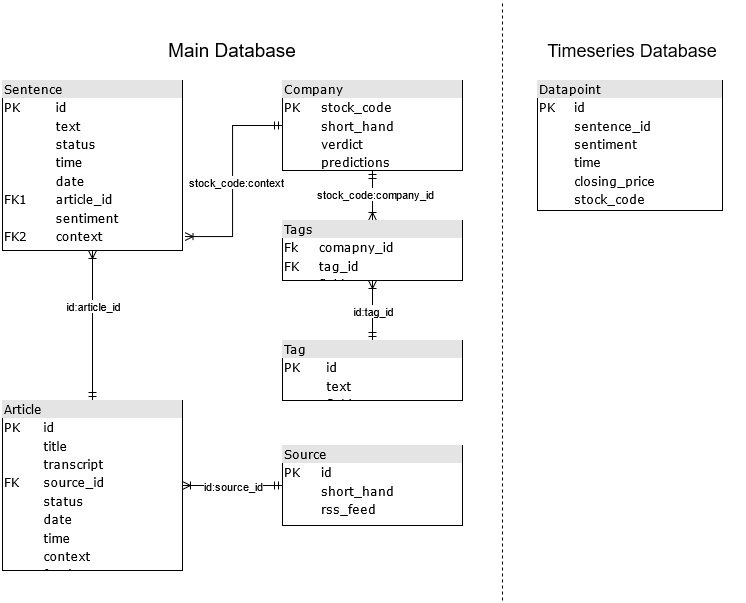
\includegraphics[width=\linewidth]{images/upload/schema.png}
    \caption{Schema of the final implementation of the main database and timeseries database}
    \label{fig:AP:schema}
\end{figure}


\chapter{System Usability Scale}
\label{Ap:SUS}

\section{Questions}

The system usability scale consists of ten question. Users are asked to assign a score to each question from 1 (strongly disagree) to 5 (strongly agree). The questions are the following: 
\begin{enumerate}
                \item I think that I would like to use this system frequently.
                \item I found the system unnecessarily complex.
                \item I thought the system was easy to use.
                \item I think that I would need the support of a technical person to be able to use this system.
                \item I found the various functions in this system were well integrated.
                \item I thought there was too much inconsistency in this system.
                \item I would imagine that most people would learn to use this system very quickly.
                \item I found the system very cumbersome to use.
                \item I felt very confident using the system.
                \item I needed to learn a lot of things before I could get going with this system.	
\end{enumerate}

\section{Results Breakdown}
\label{Ap:Results}

\begin{figure}[h]
    \centering
    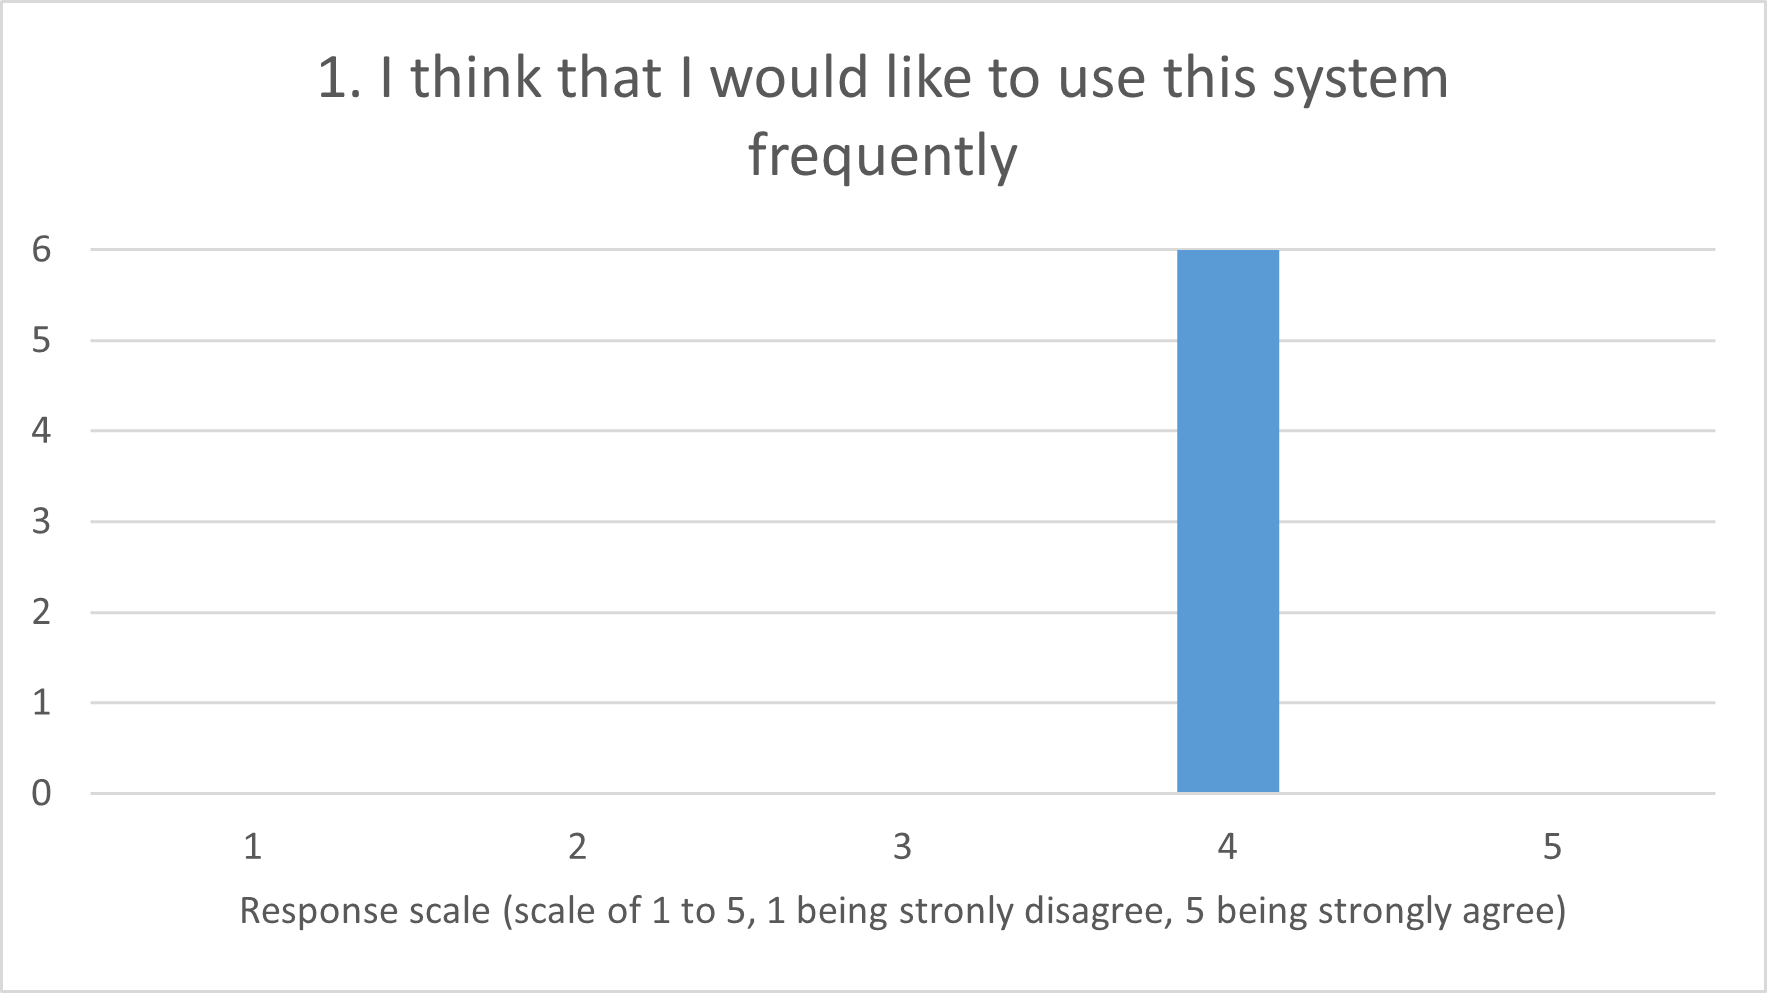
\includegraphics[width=0.7\linewidth]{images/upload/sus_results/q1.png}
    \caption{Breakdown of responses to statement "I think that I would like to use this system frequently."}
    \label{fig:q1}
\end{figure}

\begin{figure}[h]
    \centering
    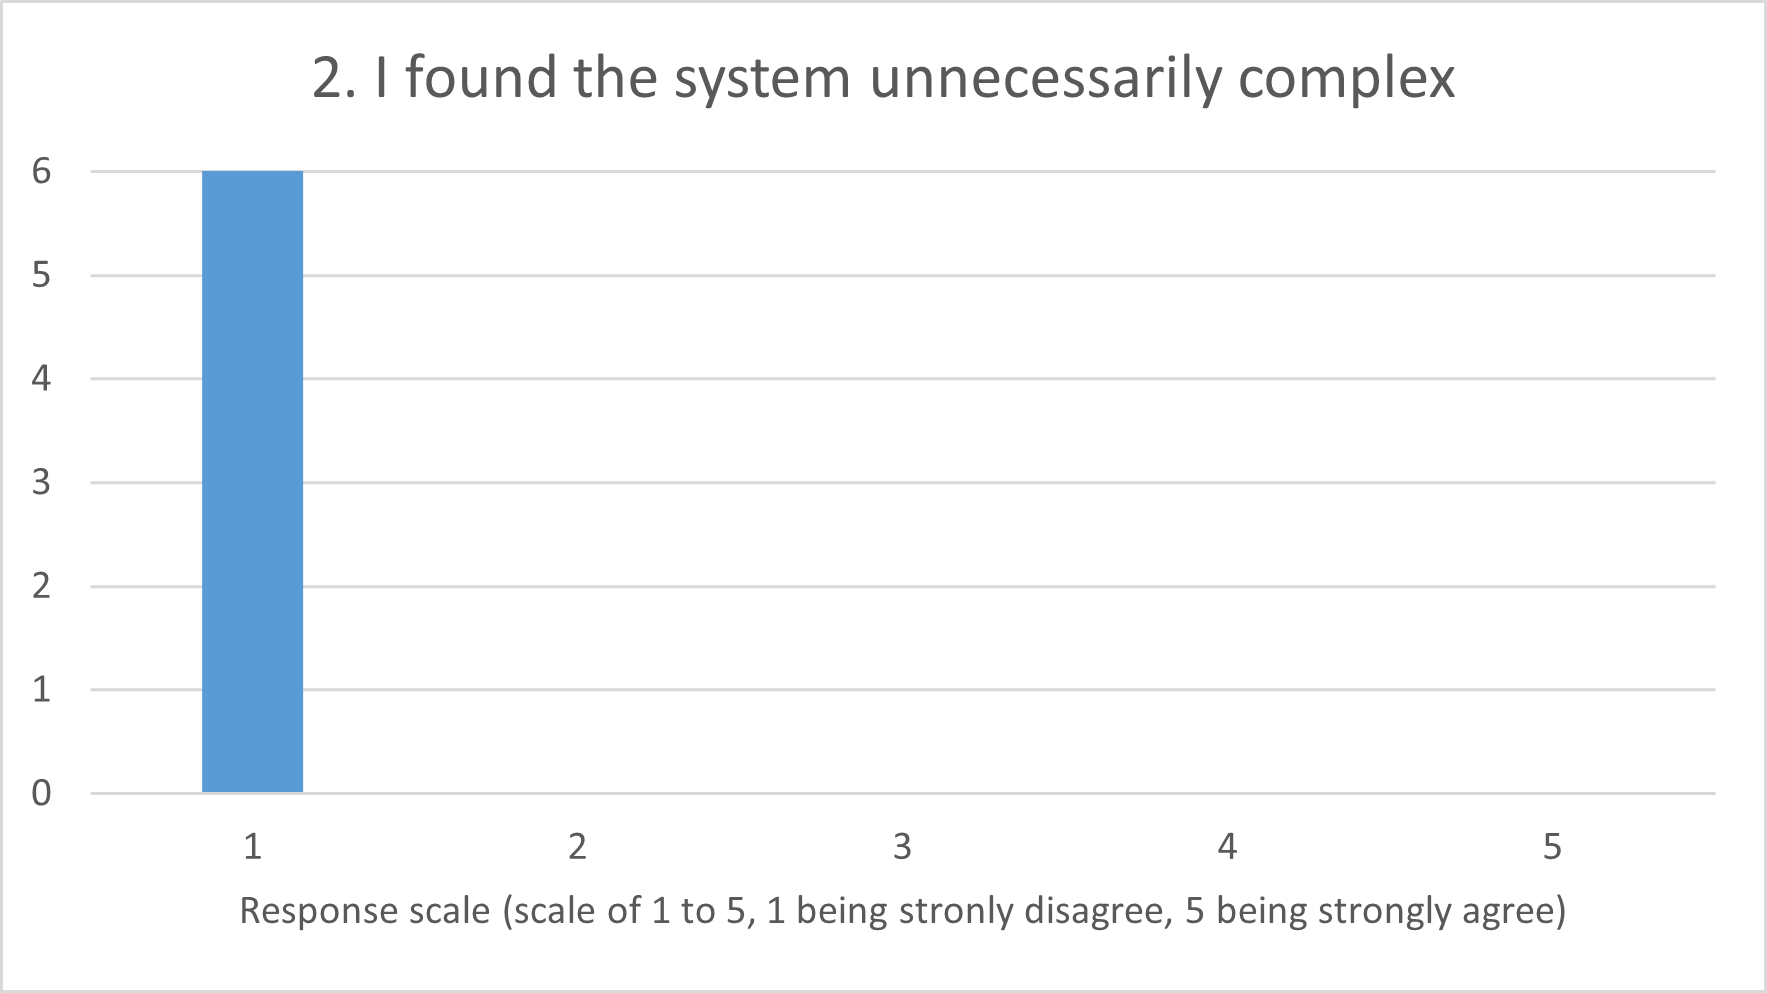
\includegraphics[width=0.7\linewidth]{images/upload/sus_results/q2.png}
    \caption{Breakdown of responses to statement "I found the system unnecessarily complex."}
    \label{fig:q2}
\end{figure}

\begin{figure}[h]
    \centering
    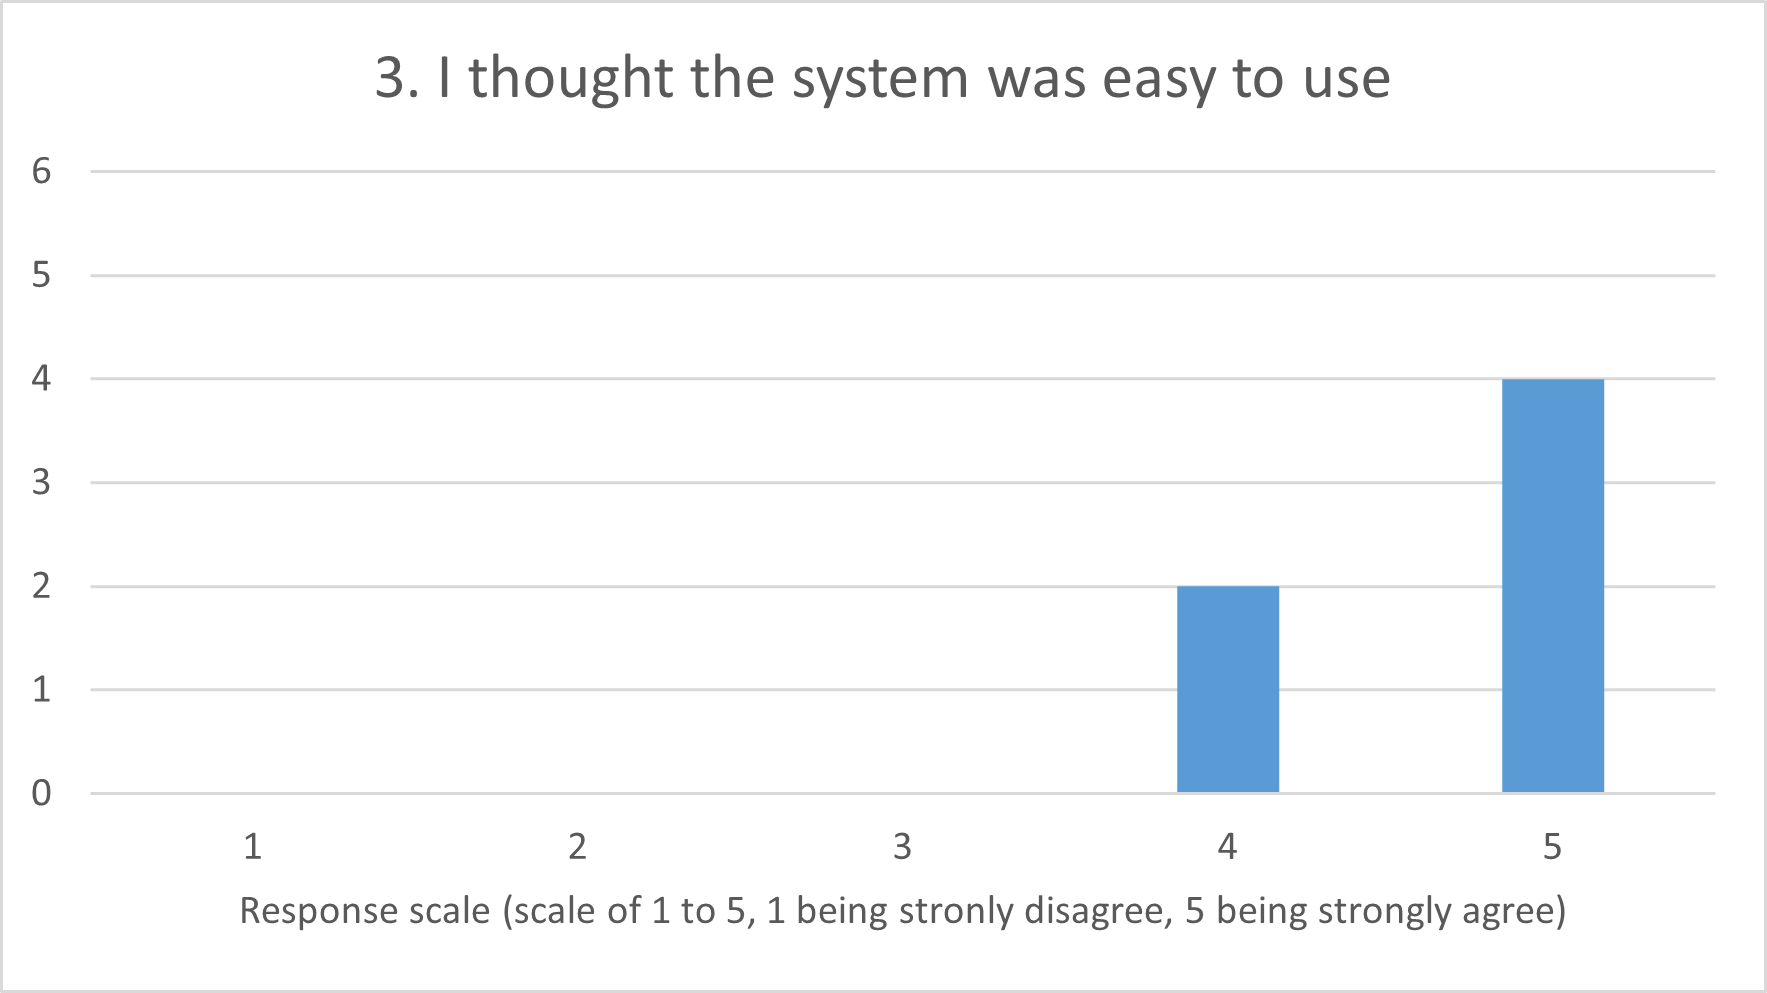
\includegraphics[width=0.7\linewidth]{images/upload/sus_results/q3.png}
    \caption{Breakdown of responses to statement "I thought the system was easy to use."}
    \label{fig:q3}
\end{figure}

\begin{figure}[h]
    \centering
    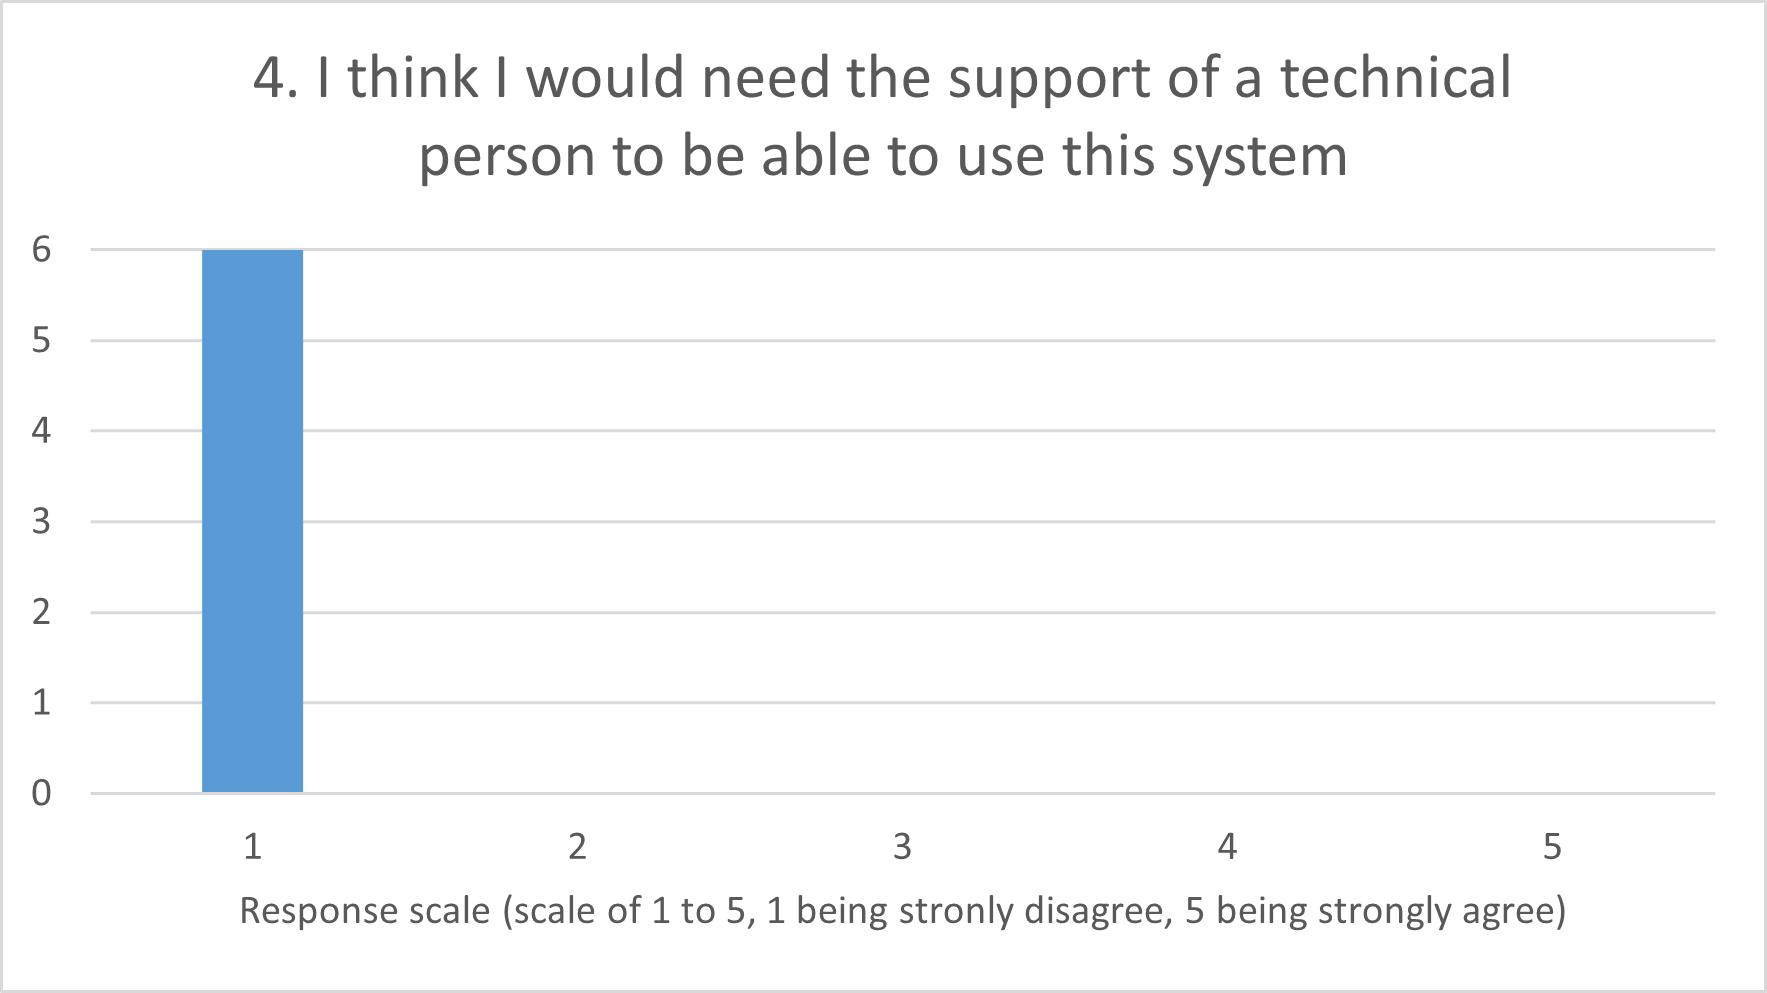
\includegraphics[width=0.7\linewidth]{images/upload/sus_results/q4.png}
    \caption{Breakdown of responses to statement "I think that I would need the support of a technical person to be able to use this system."}
    \label{fig:q4}
\end{figure}

\begin{figure}[h]
    \centering
    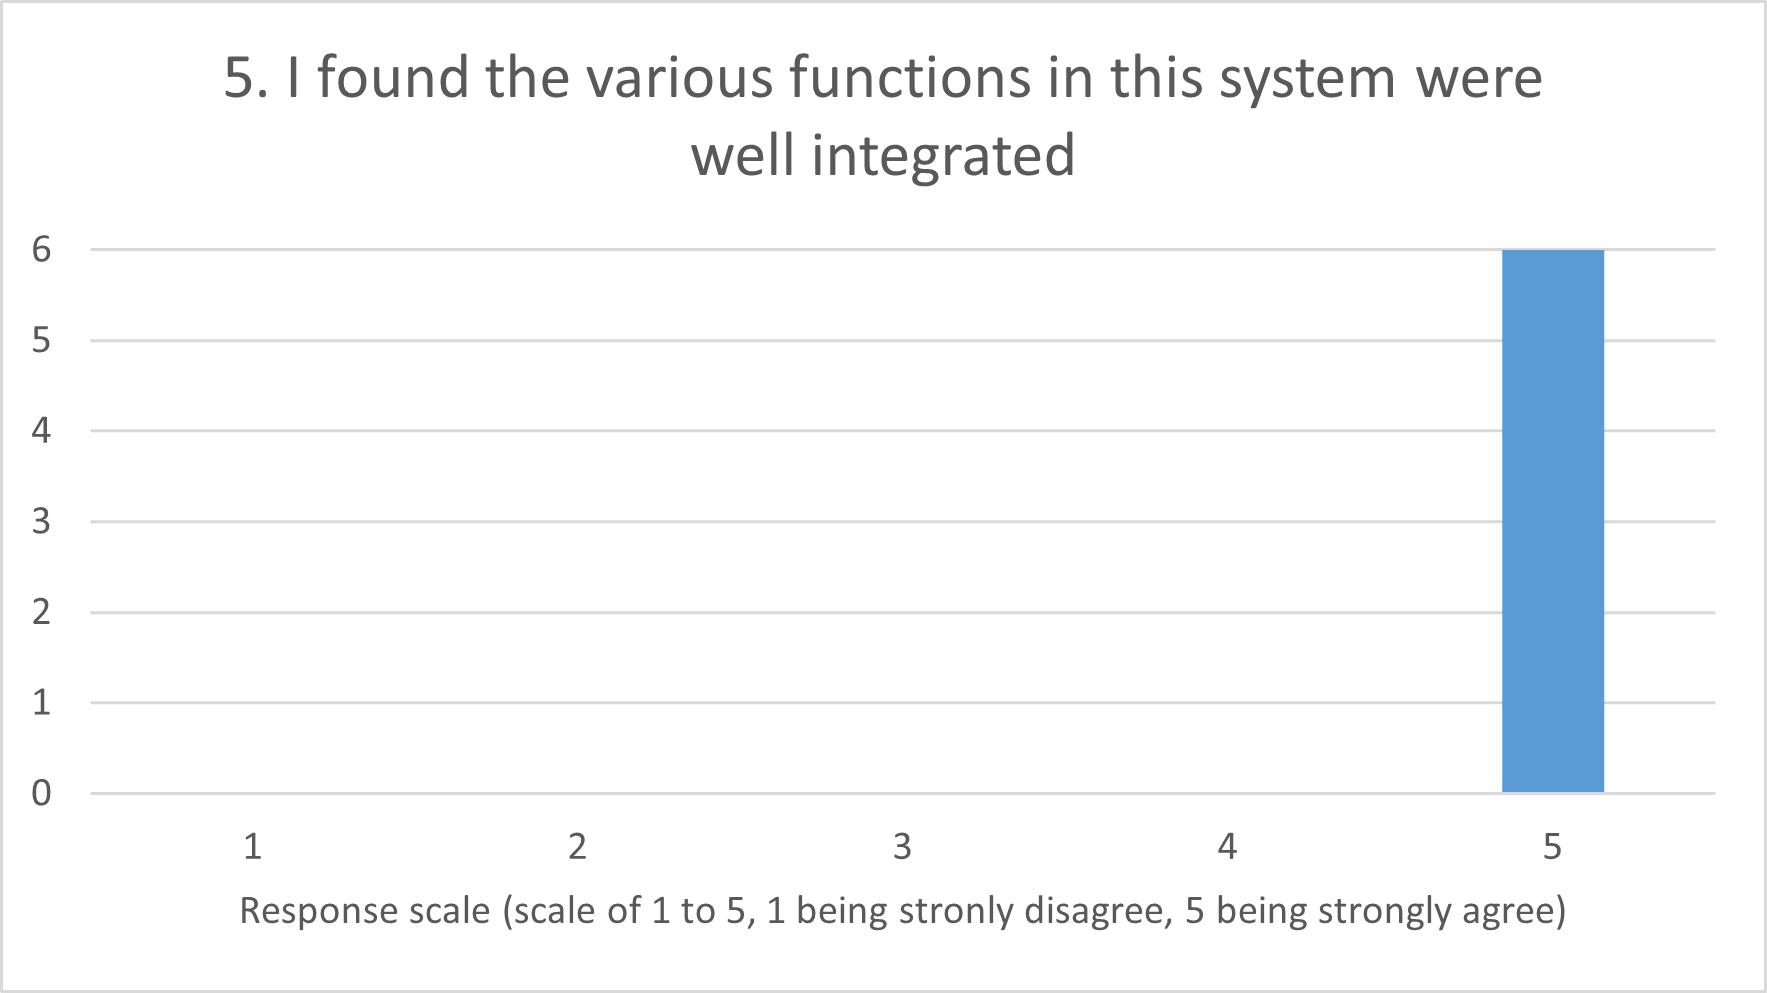
\includegraphics[width=0.7\linewidth]{images/upload/sus_results/q5.png}
    \caption{Breakdown of responses to statement "I found the various functions in this system were well integrated."}
    \label{fig:q5}
\end{figure}

\begin{figure}[h]
    \centering
    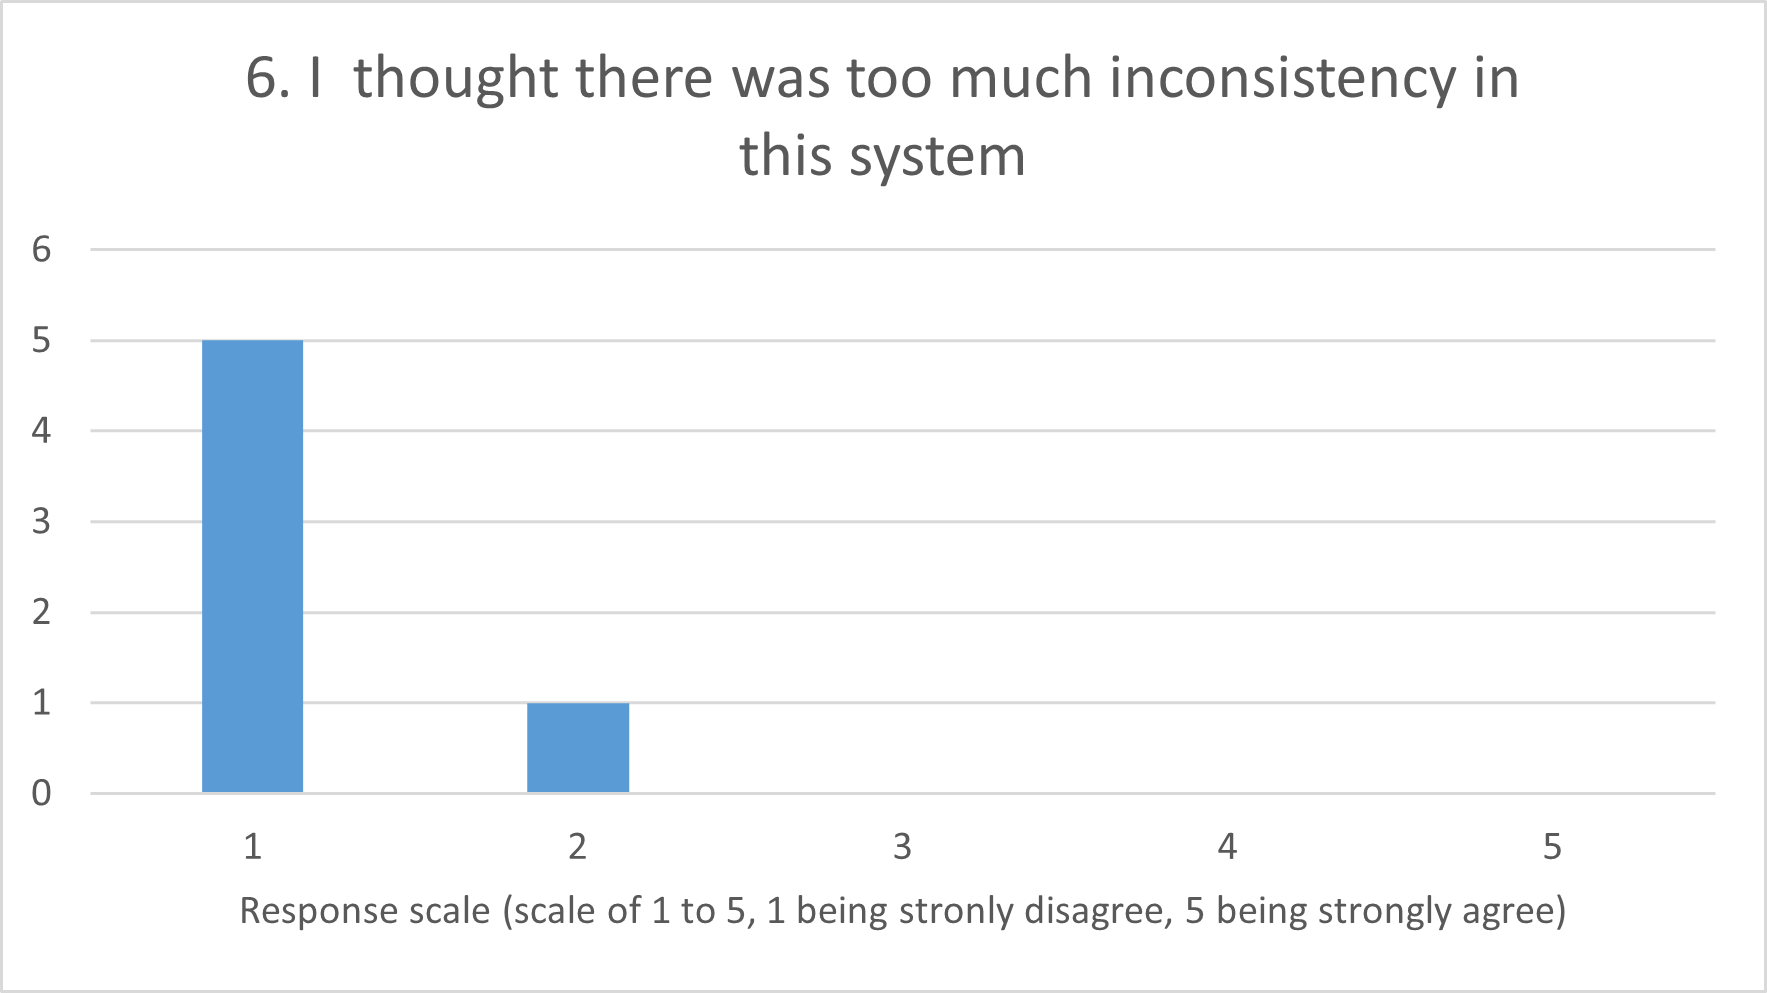
\includegraphics[width=0.7\linewidth]{images/upload/sus_results/q6.png}
    \caption{Breakdown of responses to statement "I thought there was too much inconsistency in this system."}
    \label{fig:q6}
\end{figure}

\begin{figure}[h]
    \centering
    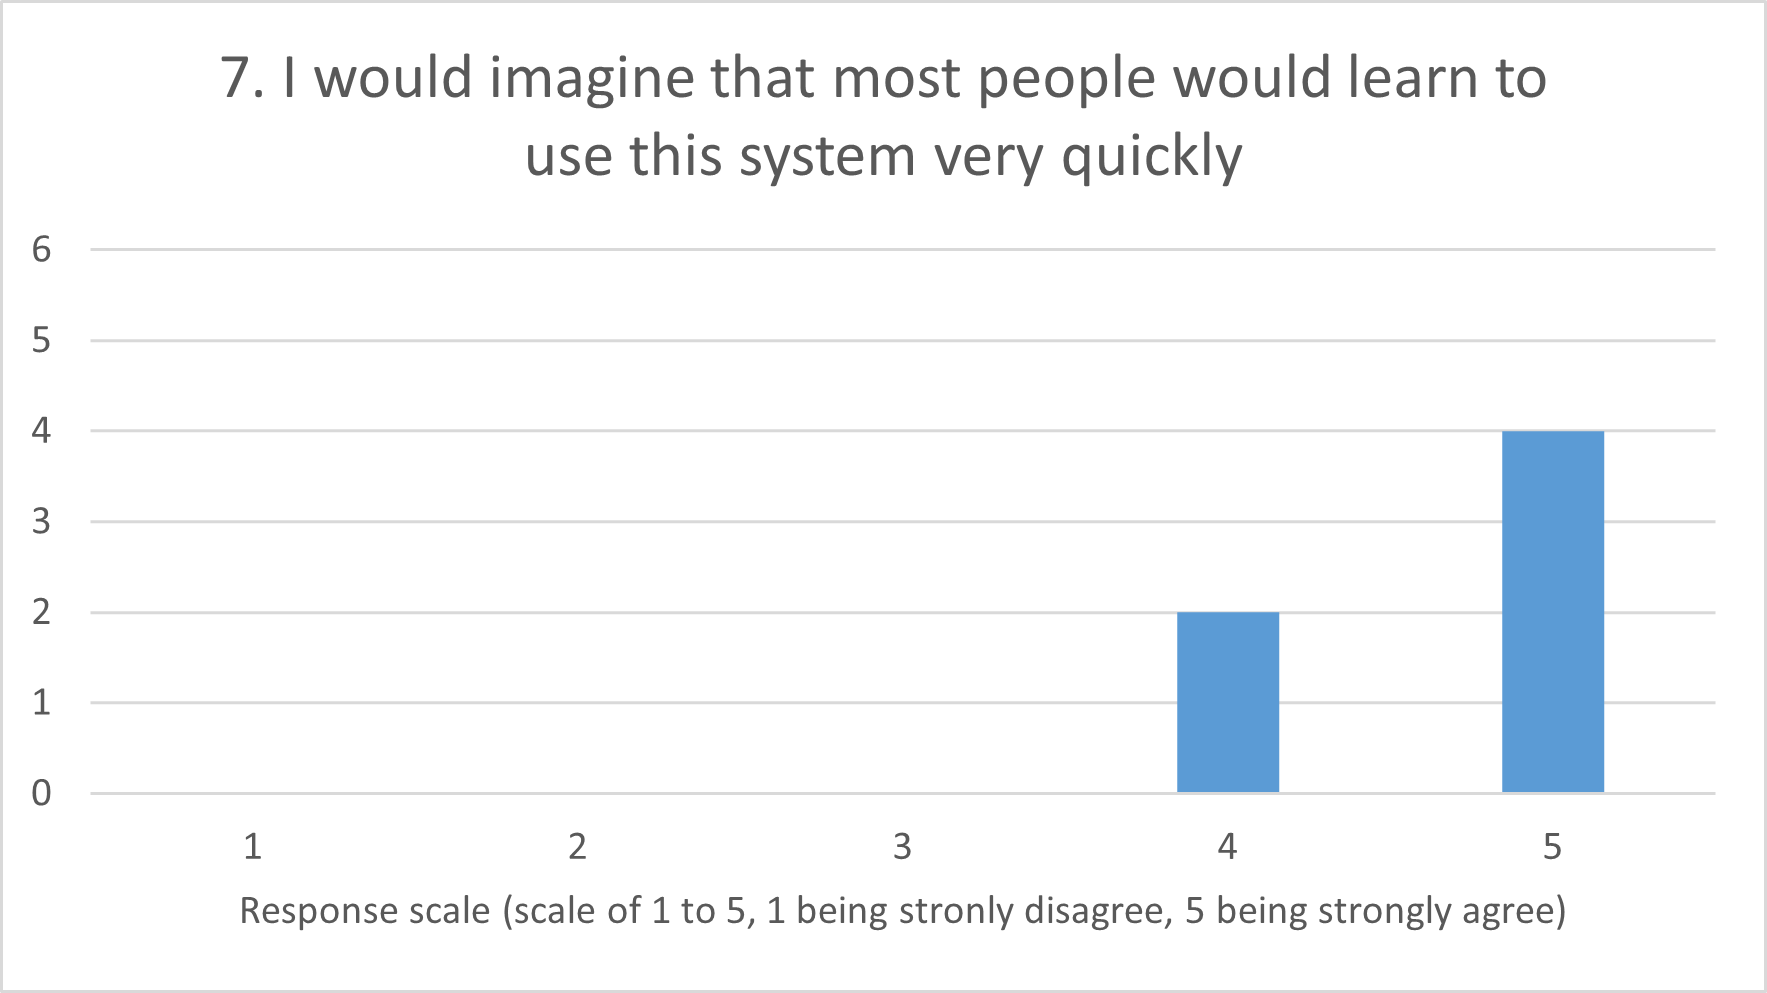
\includegraphics[width=0.7\linewidth]{images/upload/sus_results/q7.png}
    \caption{Breakdown of responses to statement "I would imagine that most people would learn to use this system very quickly."}
    \label{fig:q7}
\end{figure}

\begin{figure}[h]
    \centering
    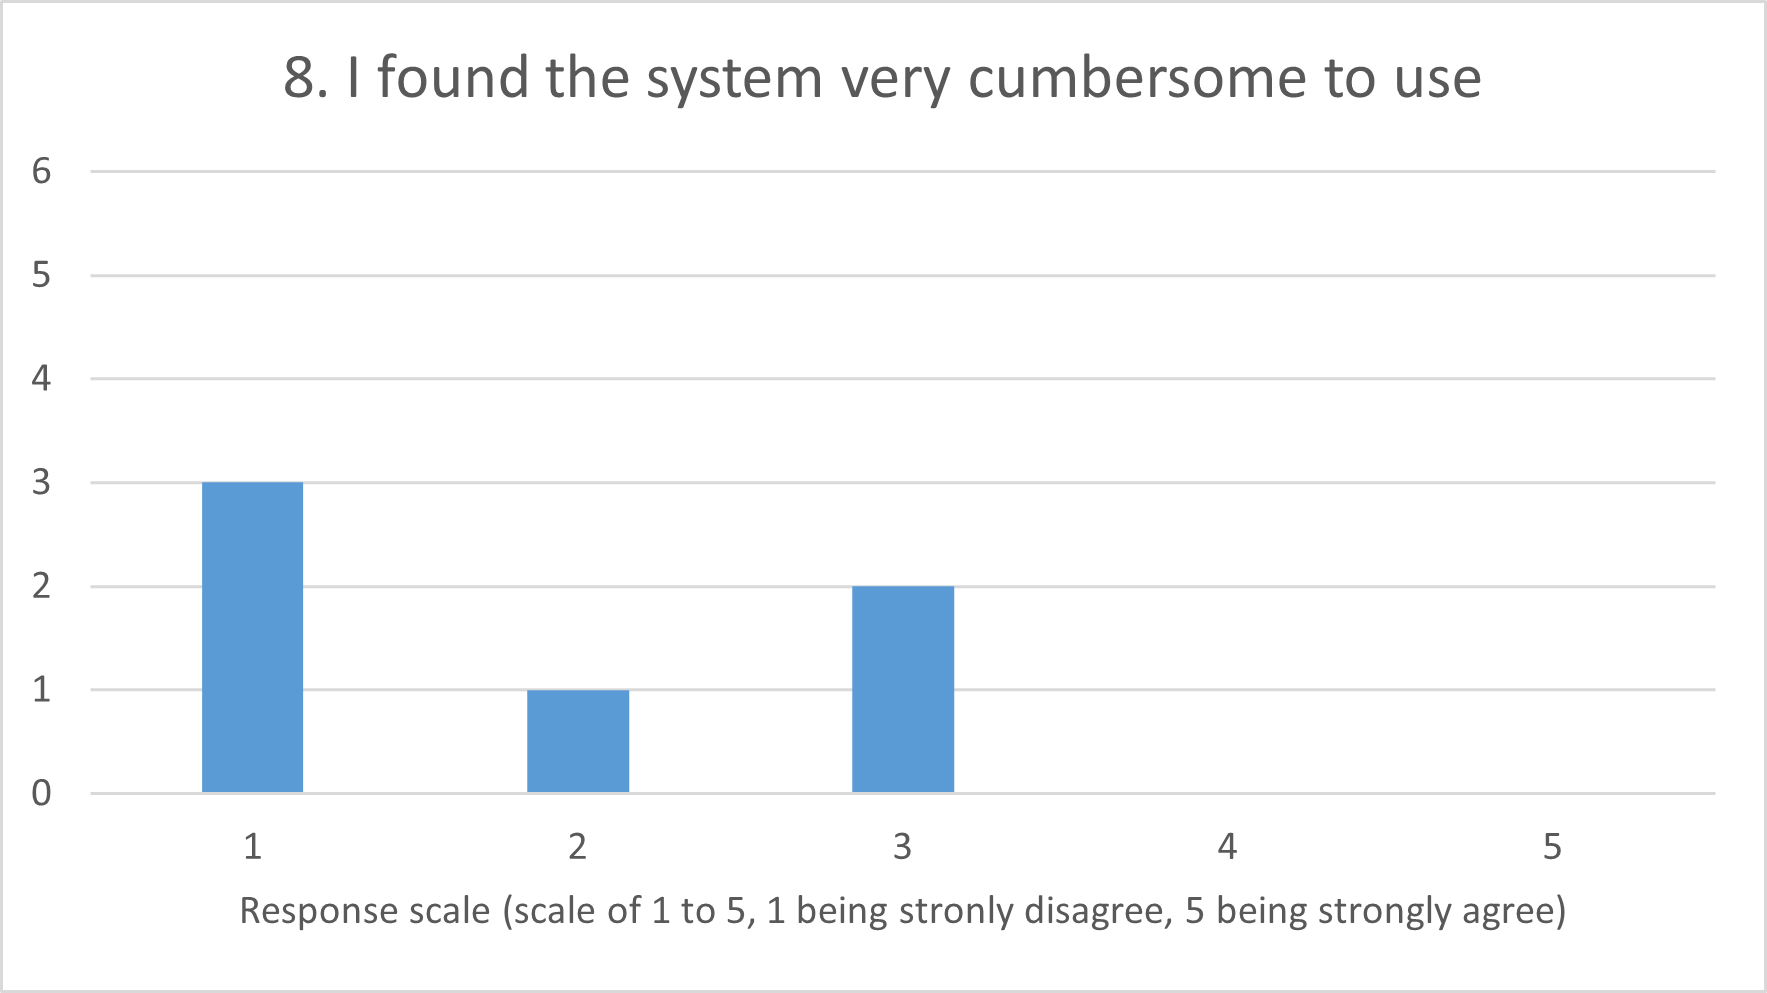
\includegraphics[width=0.7\linewidth]{images/upload/sus_results/q8.png}
    \caption{Breakdown of responses to statement "I found the system very cumbersome to use."}
    \label{fig:q8}
\end{figure}

\begin{figure}[h]
    \centering
    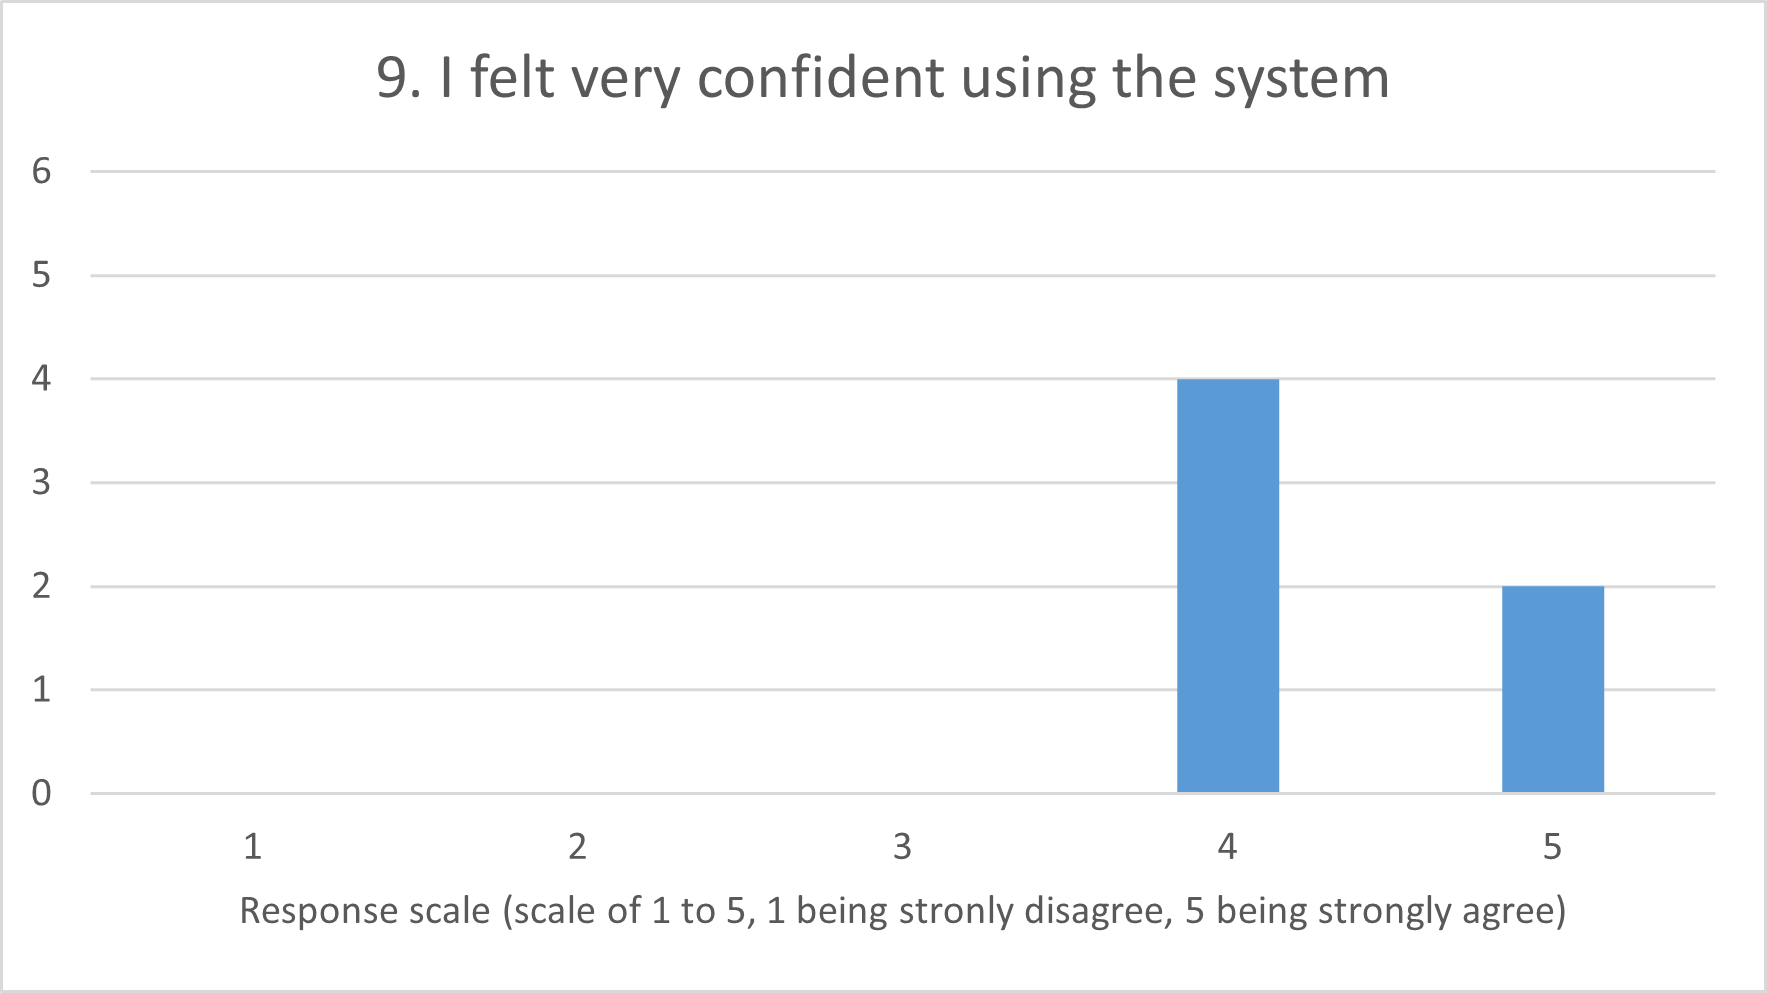
\includegraphics[width=0.7\linewidth]{images/upload/sus_results/q9.png}
    \caption{Breakdown of responses to statement "I felt very confident using the system."}
    \label{fig:q9}
\end{figure}

\begin{figure}[h]
    \centering
    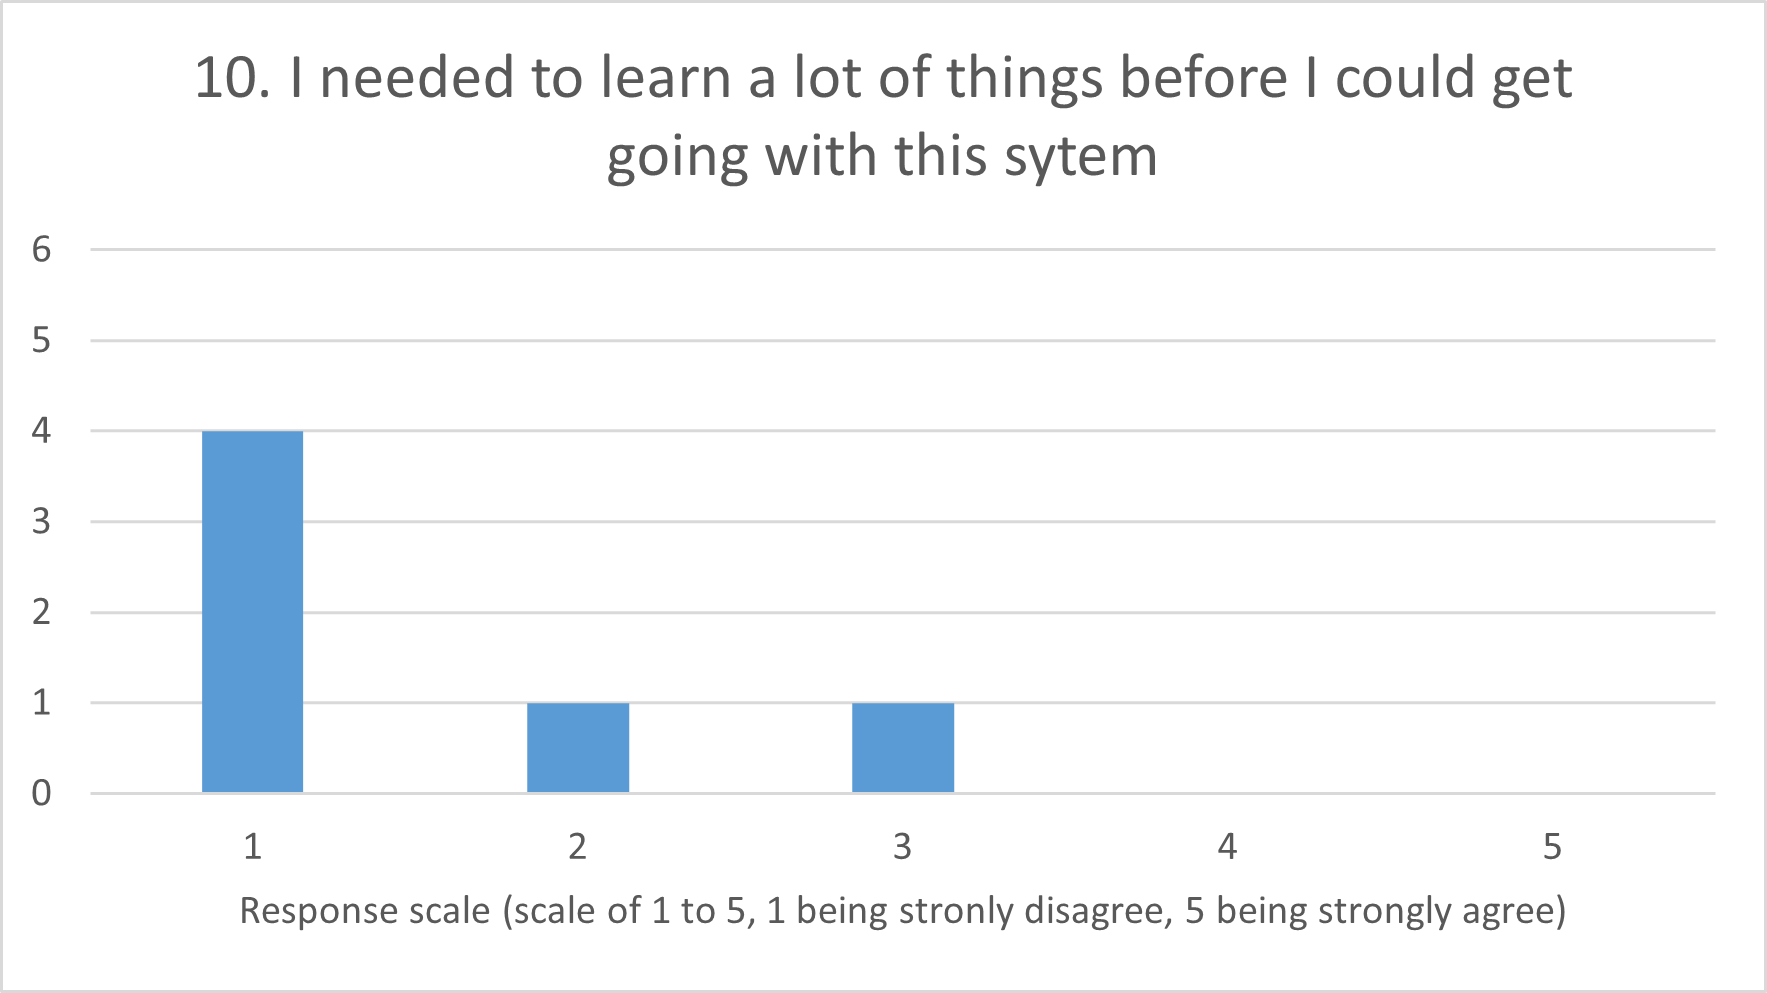
\includegraphics[width=0.7\linewidth]{images/upload/sus_results/q10.png}
    \caption{Breakdown of responses to statement "I needed to learn a lot of things before I could get going with this system."}
    \label{fig:q10}
\end{figure}



\chapter{Final Deliverable}
\label{Ap: Final Deliverable}

\subsection{Guide to Running}
Running the system is straightforward with the steps detailed below and on the project's github found here: \url{https://github.com/2312420/lvl4-project}

\begin{itemize}
    \item cd into src
    \item run docker-compose build
    \item run docker-compose up
    \item Webapp should be running at "http://127.0.0.1:8000/hotornot/"
\end{itemize}

\subsection{Final Design}
This appendix shows the home page and company page tabs that a user can access when using the webapp

\begin{figure}[h]
    \centering
    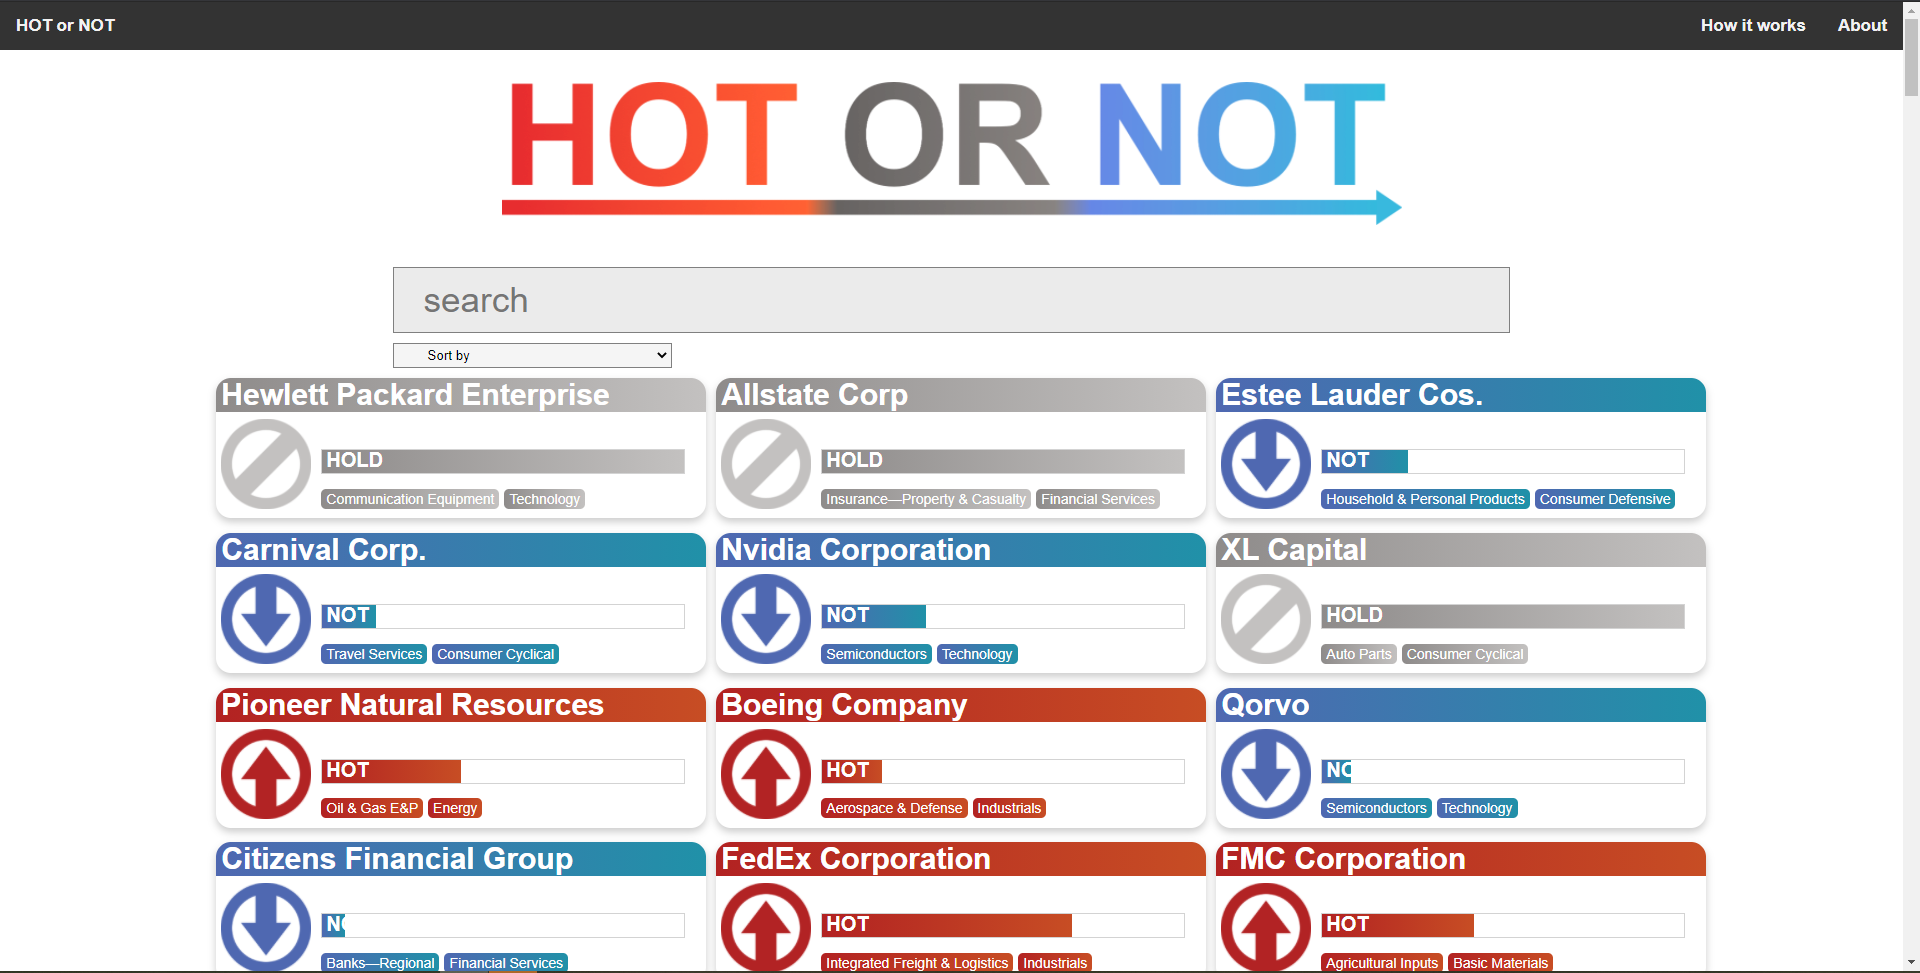
\includegraphics[width=\linewidth]{images/upload/a_homepage.PNG}
    \caption{Home page of webapp where uses can search and select companies to view }
    \label{fig:a_homepage}
\end{figure}

\bigskip

\begin{figure}[h]
    \centering
    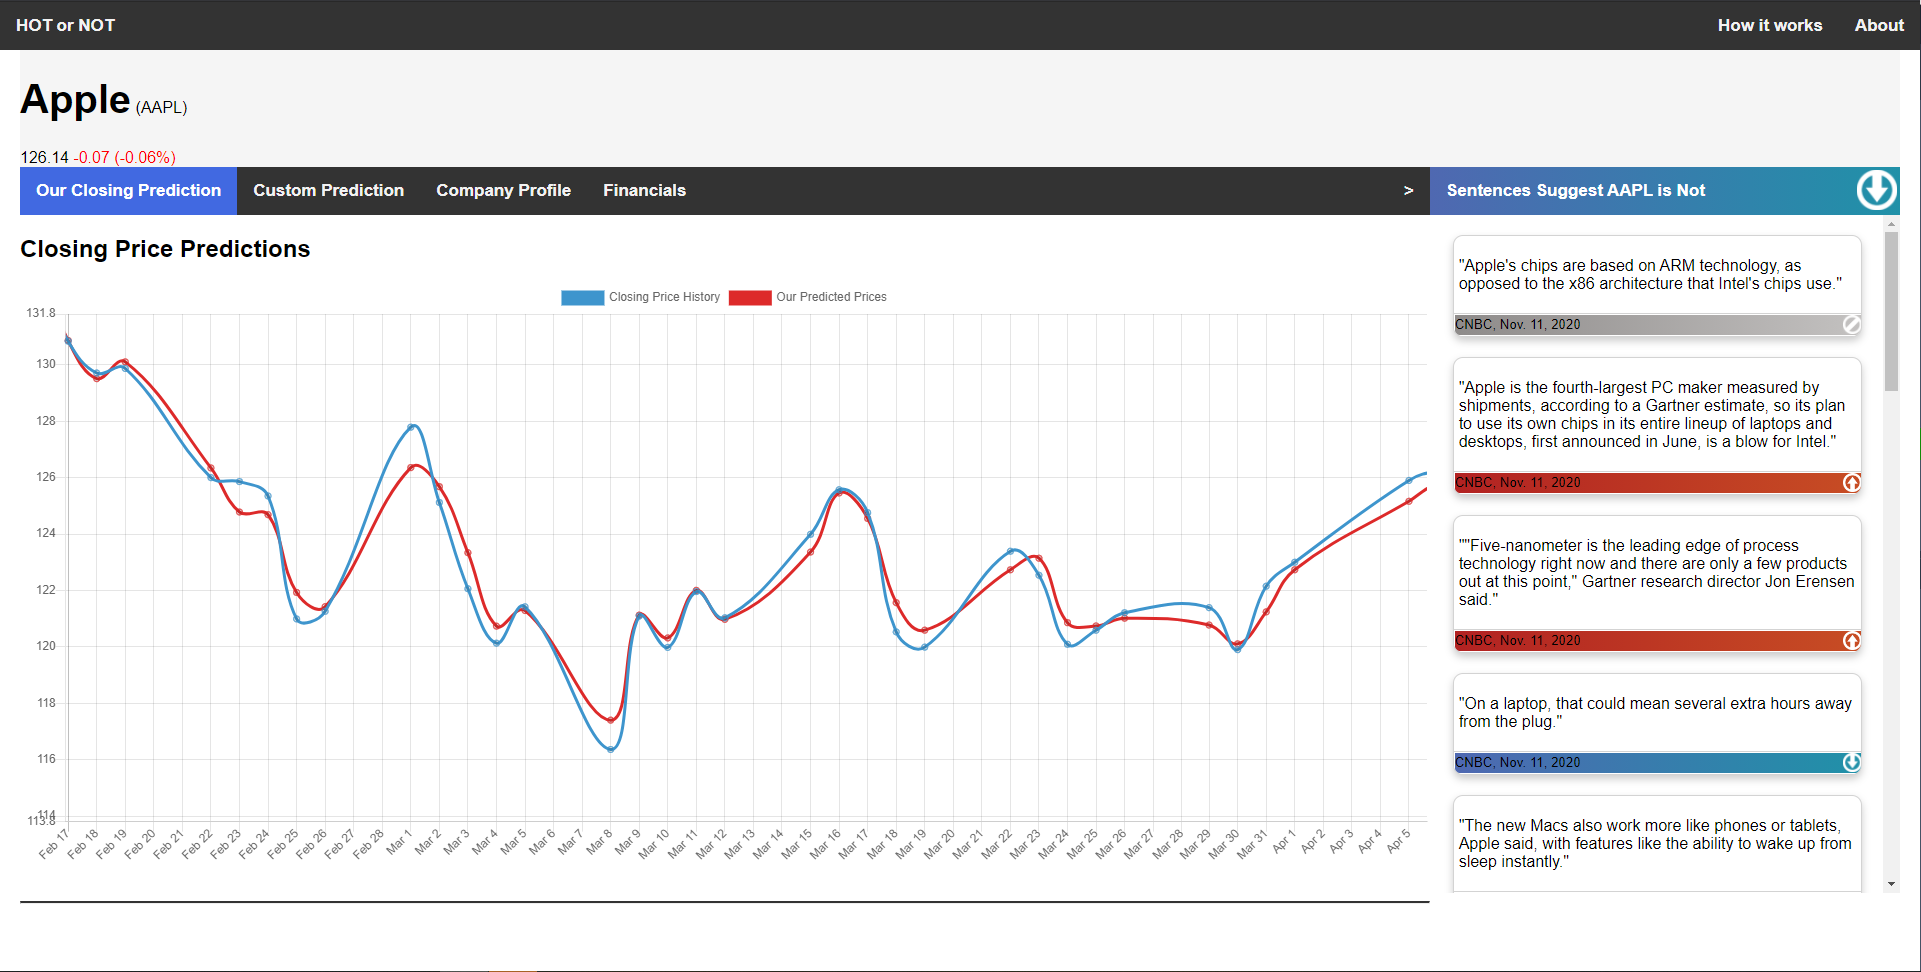
\includegraphics[width=\linewidth]{images/upload/a_ourtab.PNG}
    \caption{Company page: Our closing price predictions tab, where the default predictions are displayed }
    \label{fig:a_ourtab}
\end{figure}

\bigskip

\begin{figure}[h]
    \centering
    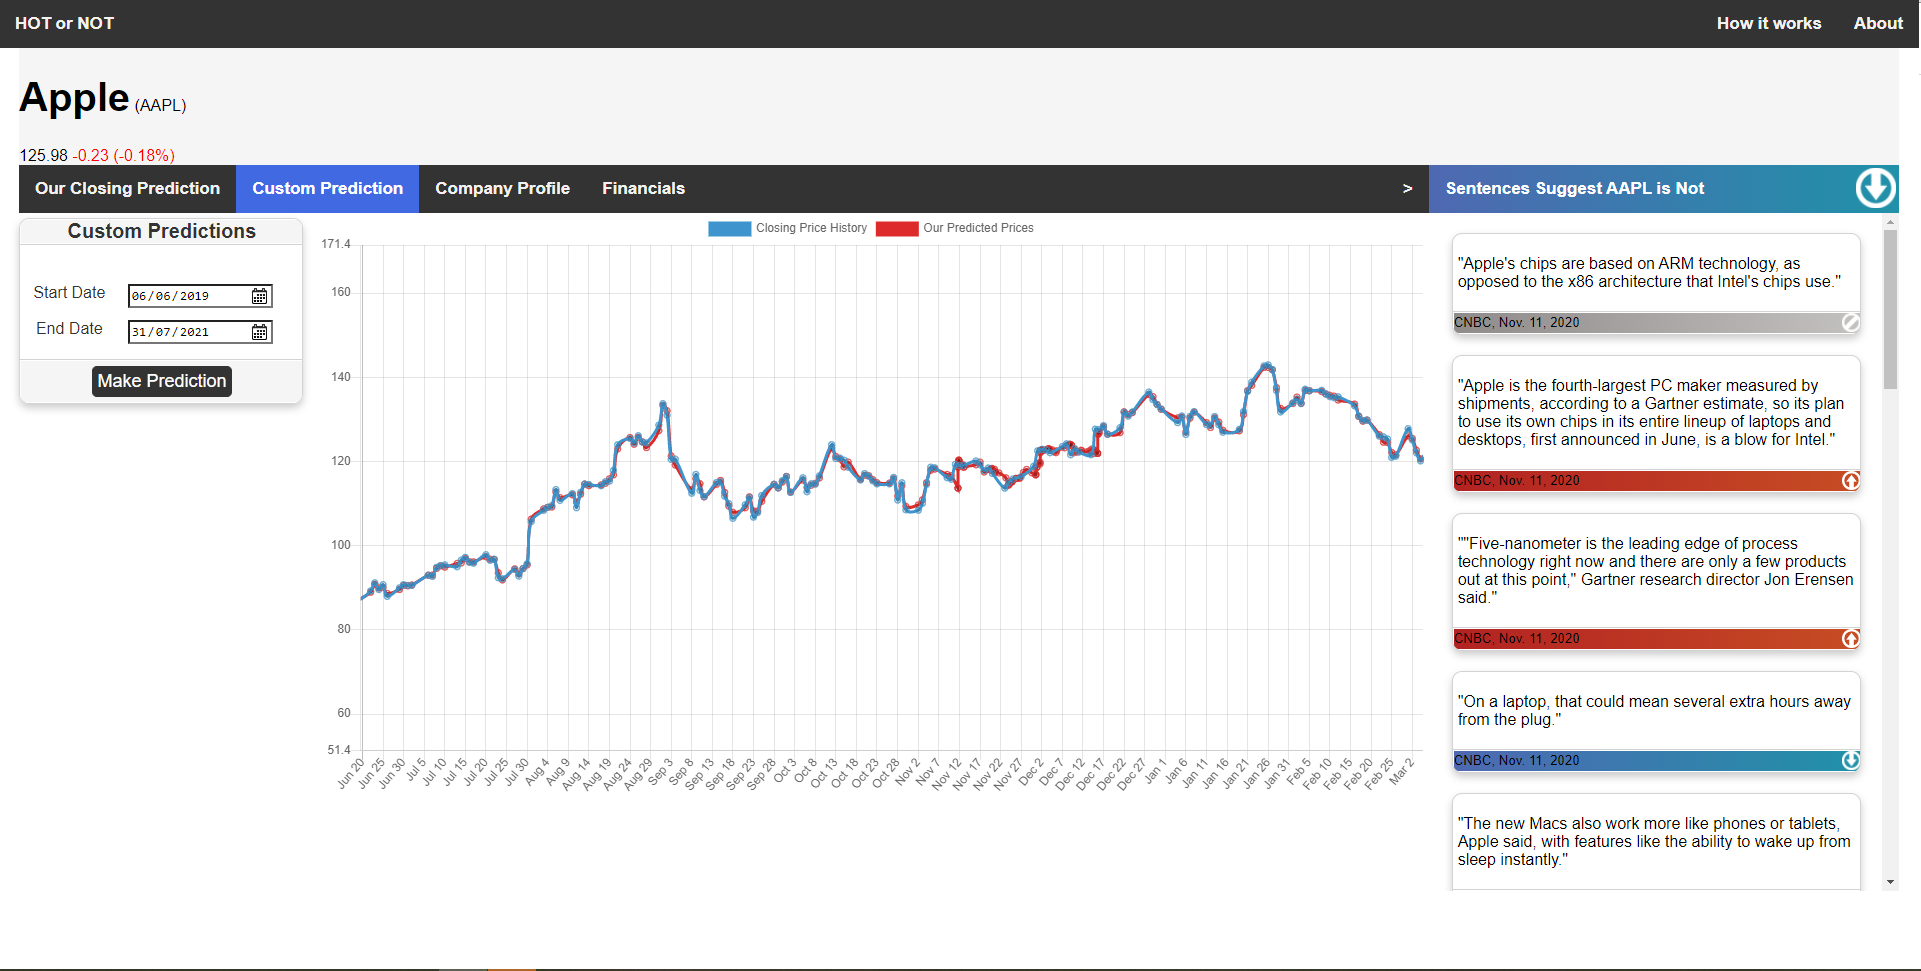
\includegraphics[width=\linewidth]{images/upload/a_customtab.PNG}
    \caption{Company page: Custom prediction tab, }
    \label{fig:a_customtab}
\end{figure}

\bigskip

\begin{figure}[h]
    \centering
    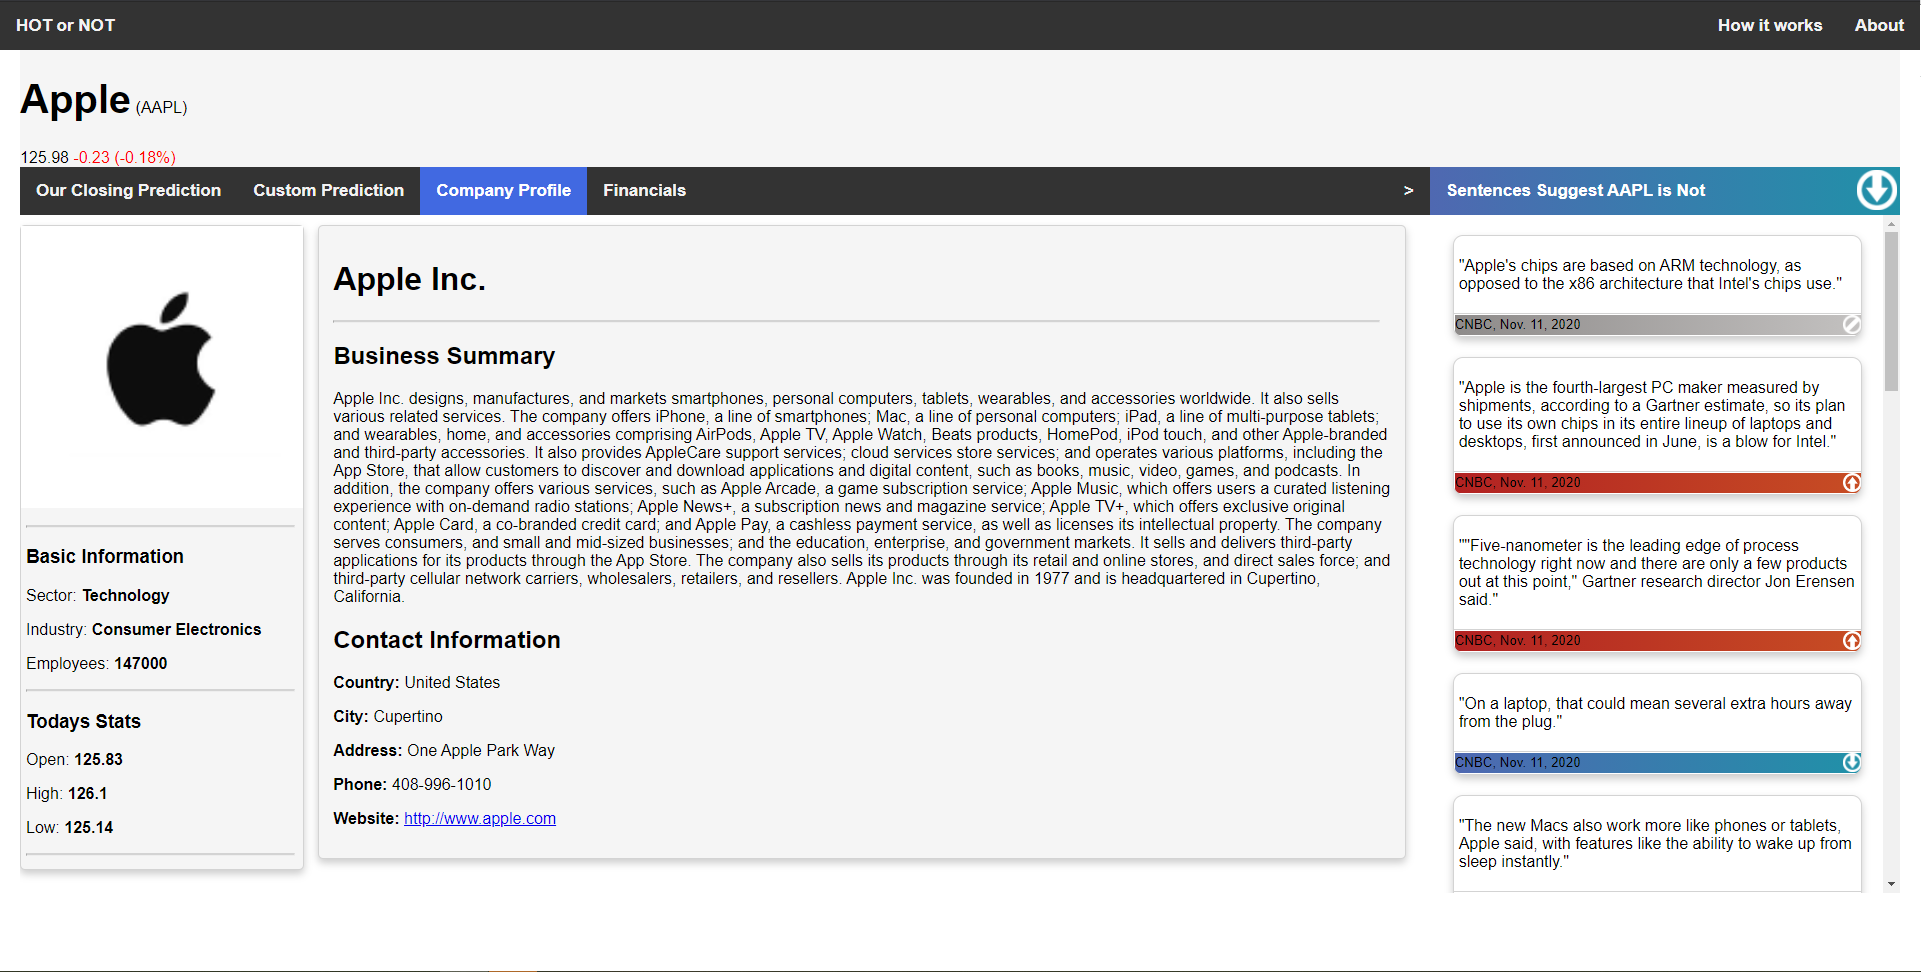
\includegraphics[width=\linewidth]{images/upload/a_profiletab.PNG}
    \caption{Company page: Company profile tab, }
    \label{fig:a_profile}
\end{figure}

\bigskip

\begin{figure}[h]
    \centering
    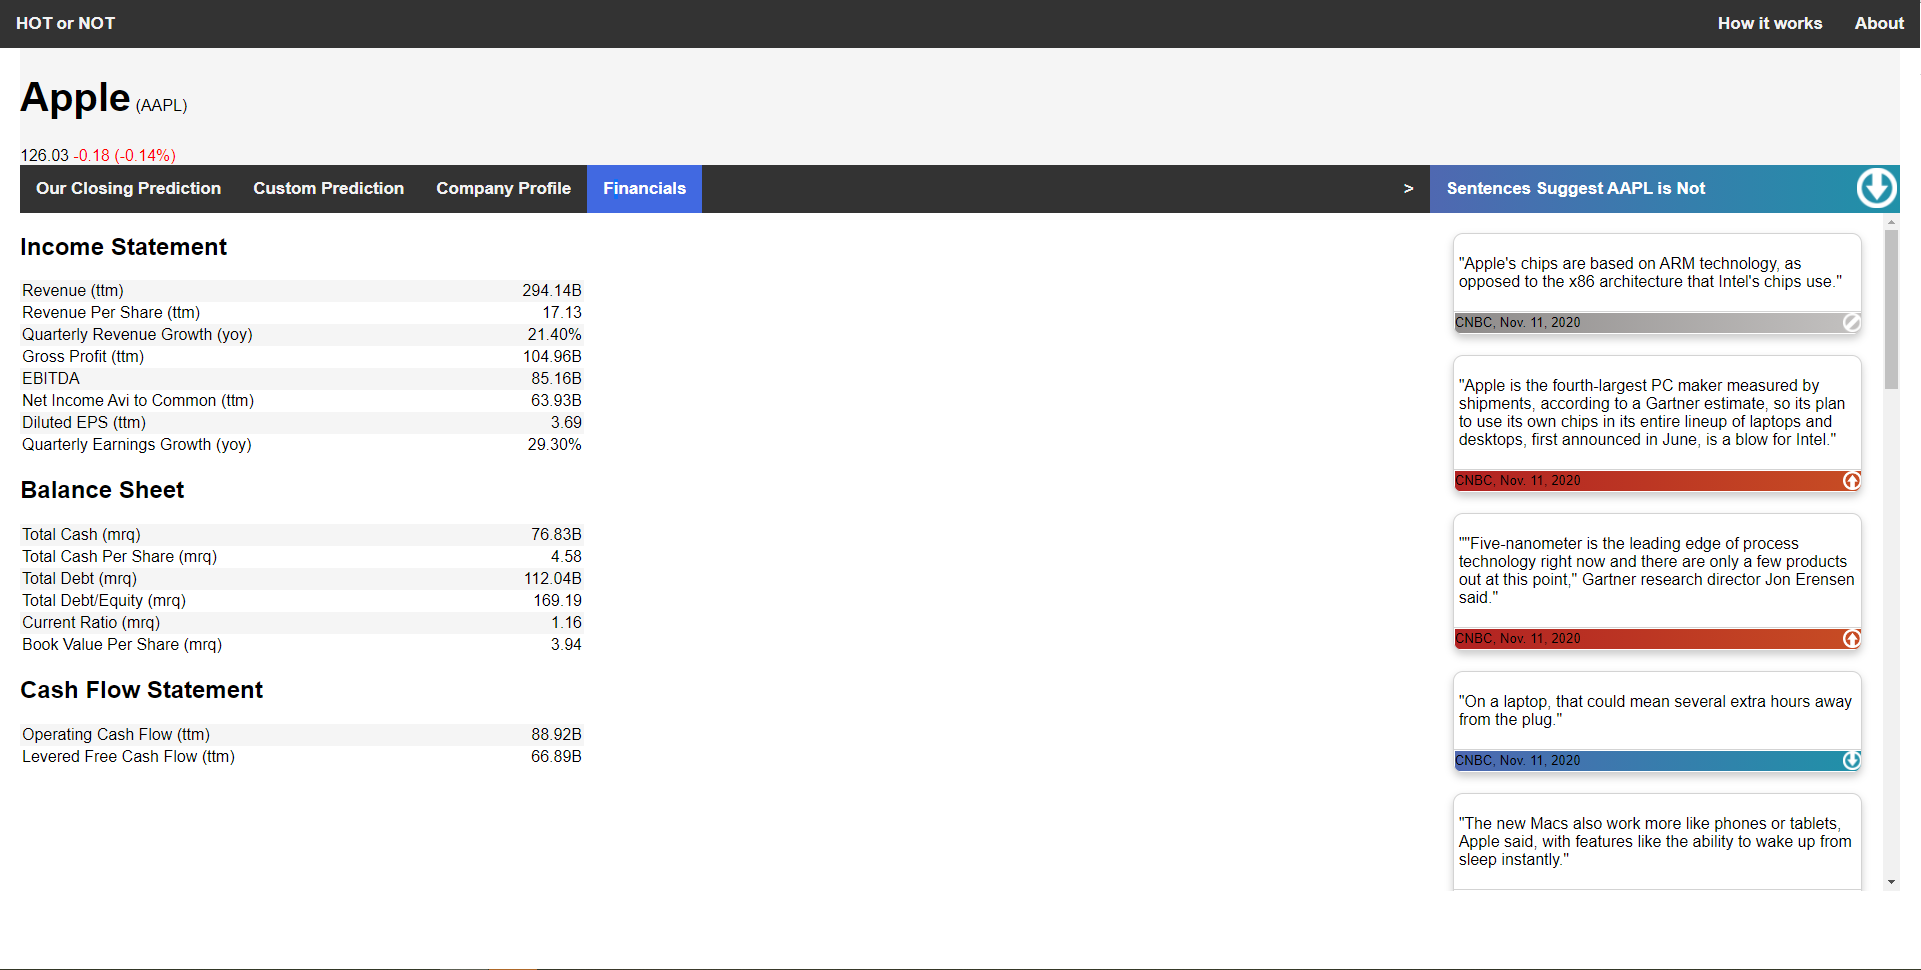
\includegraphics[width=\linewidth]{images/upload/a_fintab.PNG}
    \caption{Company page: Financials tab, }
    \label{fig:a_fin}
\end{figure}








\end{appendices}

%==================================================================================================================================
%   BIBLIOGRAPHY   

% The bibliography style is abbrvnat
% The bibliography always appears last, after the appendices.

\bibliographystyle{abbrvnat}

\bibliography{l4proj}

\end{document}
